\documentclass[twoside,english]{uiofysmaster}

\usepackage{float}	% figurer der man plasserer dem
\usepackage{caption}
\usepackage{verbatim}	% \begin{comment}
\usepackage{subcaption}
\usepackage{siunitx}
\usepackage[toc,page]{appendix}
\usepackage{minted}
\usepackage{xcolor}

\sisetup{range-phrase=-}

\usemintedstyle{borland}

\definecolor{box}{RGB}{218, 218, 218}

\setminted
{
 frame=lines, 
 fontsize=\footnotesize, 
 bgcolor=box,
}

% define lammps code listing
\lstdefinestyle{lammps}
{
  frame=single,
  keywordstyle=\ttfamily,
  keepspaces=true,
  columns=fixed,
  commentstyle=\color{black},
  stringstyle=\color{black},
  tabsize=4,
}

\lstset%
{%
 morekeywords={as},% 
 basicstyle=\footnotesize%
}%

%\bibliography{references}

\author{John-Anders Stende}
\title{Constructing high-dimensional neural network potentials for molecular dynamics}
\date{May 2017}

\begin{document}

\maketitle

\begin{abstract}
This is an abstract text.
\end{abstract}

\begin{acknowledgements}
  I acknowledge my acknowledgements.
\end{acknowledgements}

\tableofcontents

\chapter{Introduction}
***Motivate the reader, outline structure of report and what we have done***

\section{Goals}
The main goal of this thesis is to use artificial neural networks to
construct many-body potential energy surfaces (PES) to be used in molecular dyanmics (MD) simulations.  
This goal can be split into the following intermediate objecives:
\begin{itemize}
 \item Train an one-dimensional ANN with the machine learning library TensorFlow (TF) 
 to reproduce the shifted Lennard-Jones (LJ) potential.
 As a first test case, we will train the NN on random data and investigate
 how different NN architectures and activation functions influence the quality of the potential fit. 
 \item Train a many-body NN to reproduce the Stillinger-Weber (SW) potential for Si. 
 Training data (configurations of particles and energies) will be sampled from SW LAMMPS simulations. 
 The resulting NNP will then be used to simulate Si with LAMMPS. 
 We therefor need to extend the LAMMPS library with our own neural network potential.
 \item Construct a many-body NNP that will be able to simulate a system consisting of several atom types. 
 The method will be tested on the Vashishta potential for SiO2.
\end{itemize}


\part{Theory}
***Theory needed to understand the results and implementations***

\chapter{Molecular dynamics}
Molecular dynamics (MD) is a method to simulate the physical movements of atoms and molecules in gases, liquids and solids. 
It is thus a type of N-body simulation. The atoms are modelled as point-like particles with interactions described
by classical force fields. Their time-evolution is governed by Newton's equations of motion. MD allows one to study the microscopic
movement of thousands or millions of atoms, enabling the sampling of macroscopic properties such at temperature, pressure, 
diffusion, heat capacity and so on. 

The dynamics of an ensemble of particles is governed by their interactions. 
In classical MD, the interactions are described
by a classical force field $\vec{F}$, which is defined as the negative gradient of a potential energy surface (PES) $E$,
\begin{equation}
 \vec{F} = -\nabla E
\end{equation}
The PES is represented by a mathematical function, often split into a sum over two- and three-body interactions. 
Instead of using an analytical functional form to represent the energy, one can 
calculate the energies and forces for each time step in the MD simulation using an ab inito method. 
Different quantum mechanical methods like Hartree-Fock (HF) and Density Functional Theory (DFT) are used for this purpose. 
These approahces to MD are called quantum-classical molecular dynamics (QCMD). 

\section{Potential energy surfaces} \label{sec:potentialEnergySurfaces}
The dynamics of an ensemble of particles is governed by their interactions. 
In classical MD, the interactions are described
by a classical force field $\vec{F}$, which is defined as the negative gradient of a potential energy surface (PES) $E$,
\begin{equation}
 \vec{F} = -\nabla E
 \label{forcePES}
\end{equation}
The expression for $V(r)$ may be obtained in different ways:
\begin{itemize}
 \item Empirical potentials: the functional form are chosen and the parameters fitted from 
 empirical knowledge about the system
 \item Semi-empirical potentials: based on methods from computational QM, but many approximations
 are made and some parameters are obatained from empirical data
 \item Quantum mechanical potentials: a computational QM method 
 is used to obtain the energy for different configurations, and then fitted by a functional form
\end{itemize}
Instead of using a pre-defined functional form to represent the energy, one can 
calculate the energies and forces for each time step in the MD simulation using an ab inito method. 
Different quantum mechanical methods like Hartree-Fock (HF) and Density Functional Theory (DFT) are used for this purpose. 
These approahces to MD are called quantum-classical molecular dynamics (QCMD). 

The PES represents the potential energy $V(\vec{r})$ of a system as a mathematical function of the configuration of the atomic 
positions $\vec{r} = (\vec{r}_1, \vec{r}_2, \dots \vec{r}_N)$. To reduce
the $N$-body problem from a fully quantum description to a classical potential we must make the Born-Oppenheimer 
approximation, which is the assumption that the motion of atomic nuclei and electrons in a molecule
can be seperated. This enables us to freeze the degrees of freedom of the nuclei and solve the electronic
Schrödinger equation with the positions of the nuclei as parameters. Varying the positions of the nuclei
in small steps and repeatedly soving the Schrödinger equation, the quantum PES is made. 
Classically, we can now approximate the atomic nuclei as point-particles that follow
Newtonian dynamics, while the positions and velocities of the electrons are baked into the PES, usually
representing the ground state. (HA ET EGET AVNSITT OM BORN-OPPENHEIMER I KVANTETEORIDELEN KANSKJE?)

As mentioned above, we represent the PES by a pre-defined functional form in classical MD. We can assume that this
function can be written as a sum of $n$-body terms,
\begin{equation}
 V(\vec{r}) \approx \sum_{i=1}^N V_1(\vec{r}_i) + \sum_{i<j}^N V_2(\vec{r}_i, \vec{r}_j) + 
 \sum_{i<j<k}^N V_3(\vec{r}_i, \vec{r}_j, \vec{r}_k) + \dots
\end{equation}
Each term can be determined by performing an electronic structure calculation for a number of configurations, 
and fitted by a suitable functional form. Determining how many terms that is sufficient to 
describe a system adequately is however not trivial. Noble gases like argon have weak interactions and 
may be well described by a two-body potential $V_2$, while molecules with strong angular dependencies on their bond, like
silicon (Si), will need at least three-body potentials $V_3$. Another challenge is to identify the
configuration space of the system. For three-body potentials and more the set of probable configurations is large, and 
running an \textit{ab inito} simulation for each configuration is expensive. This problem will be discussed below. 

An important step is how to fit the above potential terms obtained from QM calculations to a functional form. 
There exist a lot of different interpolation teqhniques; in this theses we will use ANNs to fit the data. 
(SKRIVE OM ANDRE INTERPOLASJONSTEKNIKKER?)




\chapter{Machine learning}
Machine learning is the science of giving computers the ability to learn without being explicitly programmed. 
The idea is that there exist generic algorithms which can be used to find patterns in a broad class of data sets without 
having to write code specifically for each problem. The algorithm will build its own logic based on the data. 

There are two main machine learning methods, supervised learning and unsupervised learning. For the former method, 
you know the answer to a problem and let the computer deduce the logic behind it. When doing the latter, you do not
know the answer and are just trying to find patterns and relationship in the data. 

Another way to categorize machine learning tasks is to consider the desired output of a system.
Some of the most common tasks are:
\begin{itemize}
 \item Classification: Outputs are divided into two or more classes. The goal is to 
 produce a model that assigns inputs into one of these classes. An example is to identify
 digits based on pictures of hand-written ones. Typically supervised. 
 \item Regression: Find a functional relationship between variables, the outputs are thus continous. 
 \item Clustering: Inputs are divided into groups without knowing the different groups, i.e. a form of unsupervised classification.  
\end{itemize}
In this thesis we will use machine learning to do regression, i.e. to find the PES of interacting molecules.
One approach to machine learning regression is artificial neural networks. 

\section{Artificial Neural Networks} \label{sec:ANN}
An Artificial Neural Network (ANN) consists of layers of connected nodes, or neurons. 
It is supposed to mimic a biological nervous system by letting each neuron interact with other neurons
by sending signals between layers. The accumulated signals received by a neuron is used as input to its 
\textit{activation function}, which is used to to send new signals to following layers. This function is supposed to mimic that 
a biological neuron is activated if the input is above a certain threshold. We will here follow 
Behler \cite{Behler11general} and Dragly \cite{Dragly14}.

There are many types of ANNs made for different purposes. The most widely used are feed-forward and recurrent ANNs. 
The feedforward network was the first and arguably the most simple type of ANN. In this network the information or signals
only move forward through the layers - from the input layer, through each successive hidden layer and finally to the output layer. 
On the other hand, recurrent networks have cycles and loops, i.e. bi-directional data flow. Feed-forward neural networks, 
also called Multilayer Perceptrons (MLP) were shown to be universal function approximators by K. Hornik et al. \cite{Hornik89} in 1989.
We will use these networks to approximate the PES in thesis. 
\begin{figure}[H]
\begin{center}
  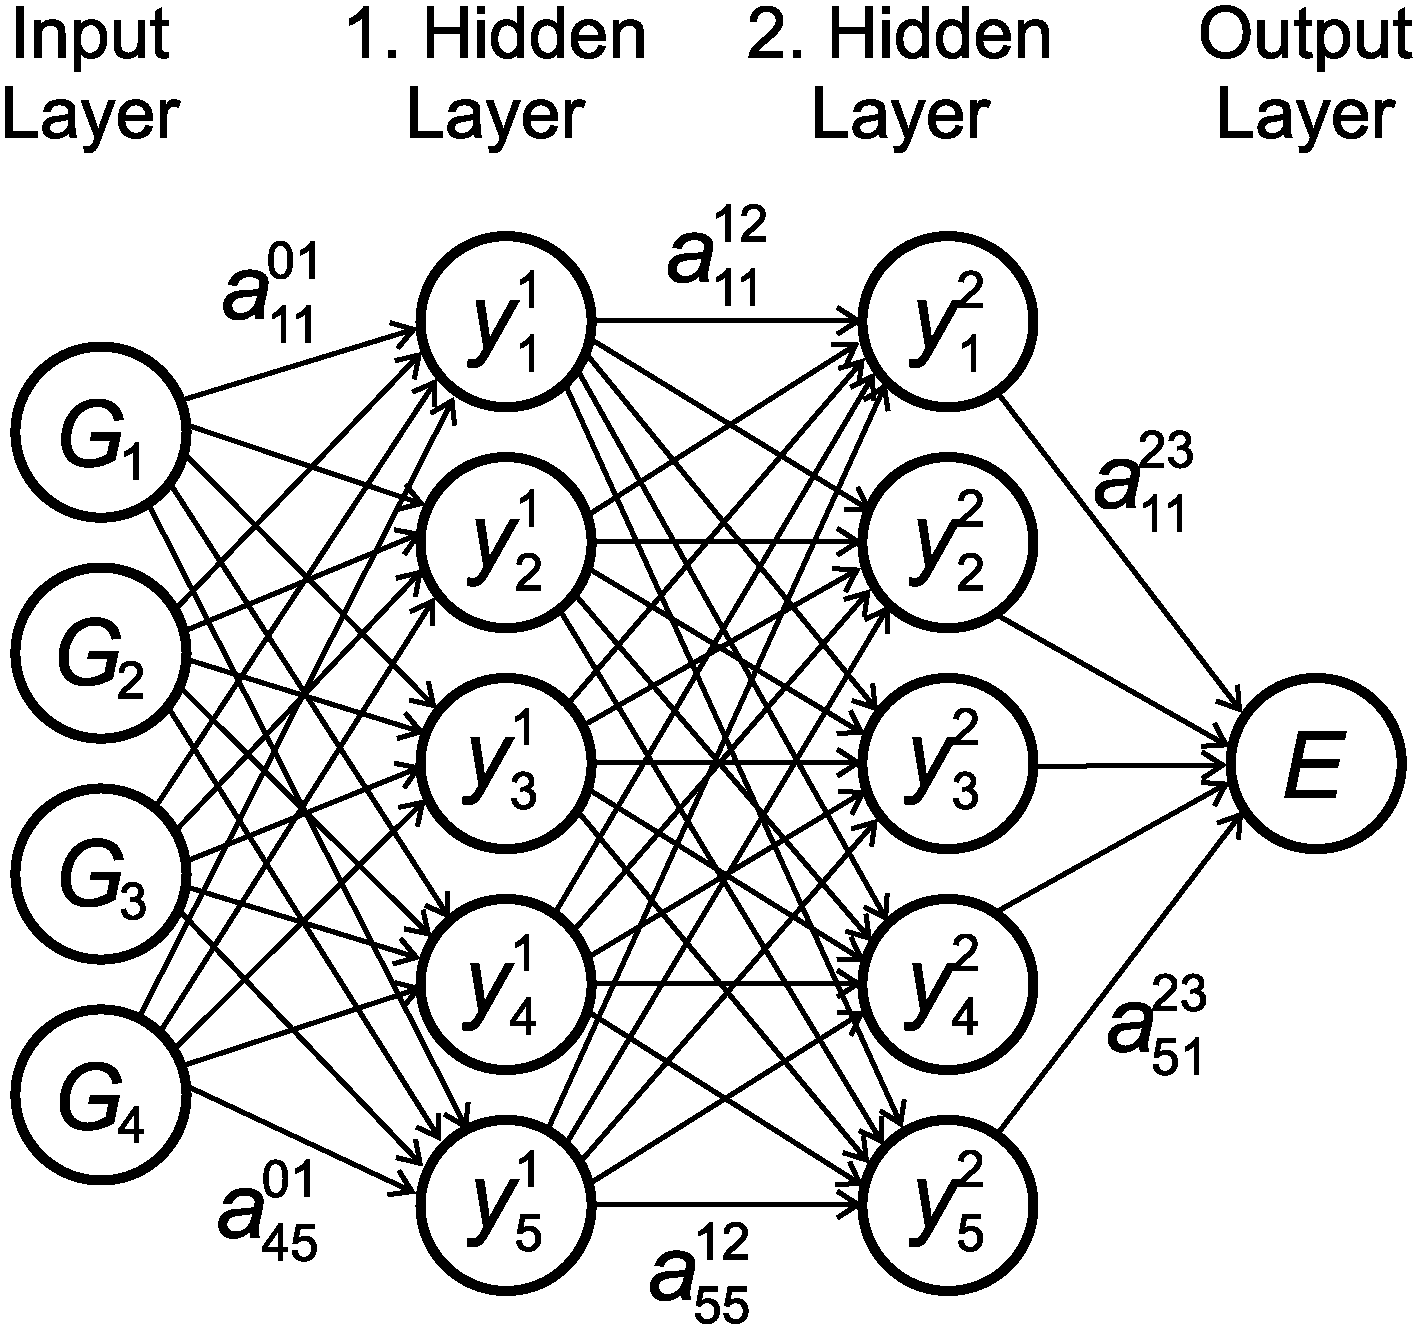
\includegraphics[width = 0.7\linewidth]{Figures/Theory/MLP.png}
  \caption{Neural network}
  \label{fig:NN}
  \end{center}
\end{figure}
An MLP networks is shown schematically in \autoref{fig:NN} (STOLEN FROM \cite{Behler11general}, EDIT TO ONE INPUT LATER). 

This network maps input coordinates $G_i$ to a potential energy in the output layer via two hidden layers
with an (arbitrary) number of hidden nodes. The hidden neurons have no physical meaning, but have the purpose
of defining the functional form of the NN. All nodes in each layer are connected to the nodes in the adjacent layer by
\textit{weights}, the fitting parameters of the NN. These are called fully connected layers. We use the notation
$a_{ij}^{kl}$ for the weight connecting node number $i$ in layer $k$ with node number $k$ in layer $l=k+1$. 
Also, each node in the hidden layers and the output node have a \textit{bias} $b_i^j$, where $i$ indicates
node number and $j$ layer. All weights and biases are real-valued numbers.

The output of this MLP is calculated in the following way. The configuration are specifiec by the input nodes.
Then, a weighted sum $x_m^1$ of the input coordinates ${G_i}$ is calculated for each node $m$ in the first hidden layer 1
\begin{equation}
 x_m^i = \sum_{i=1}^4 G_i a_{i,m}^{01} + b_m^i 
\end{equation}
where we also add the bias $b_m^i$ for each node. This is a linear combination of the input coordinates
using the connection weights as coordinates, which is used as input to the activation function $f_m^1$ of each neuron, thus
producing the output $y_m^1$ of all neurons in layer 1:
\begin{equation}
 y_m^1 = f_m^1(x_m^1)
\end{equation}
For an arbitrary node $m$ in a hidden layer $n$ this generalizes to
\begin{equation}
 y_m^n = f_m^n(x_m^n) = f_m^n\left(\sum_{i=1}^{N_{n-1}} y_i^{n-1}a_{i,m}^{n-1,n}\right)
\end{equation}
where $N_n$ is the number of nodes in layer $n$. When the output of all the nodes in the first hidden layer are computed,
the values of the subsequent layer can be calculated and so forth until the output is obtained. The complete functional form
of an MPL with $n$ hidden layers is thus
\begin{equation}
 E = f_1^{n+1}\biggr(\sum_m^{N_n}f_m^{n}\biggr(\sum_l^{N_{n-1}}f_l^{n-1}\biggr( \cdots \sum_j^{N_1} 
     f_j^1\biggr(\sum_{i=1}a_{i,j}^{0,1}G_i + b_j^1\biggr) \cdots \biggr)\biggr)\biggr)
     \label{completeNN}
\end{equation}
i.e. a nested sum of activation functions. A desired property of activation functions is to converge asymptotically
to constant output values for large and small arguments, with a non-linear region in-between. The non-linearity enables
the ANN to fit arbitrary functions \cite{Hornik89}. Common activation functions \cite{Rojas96} for 
function approximation are the sigmoid function
\begin{equation}
 f(x) = \frac{1}{1 + e^{-x}}
 \label{sigmoidActivationFunction}
\end{equation}
and the hyperbolic tangent
\begin{equation}
 f(x) = \tanh(x)
 \label{tanhActivationFunction}
\end{equation}
\begin{figure}[H]
\begin{center}
  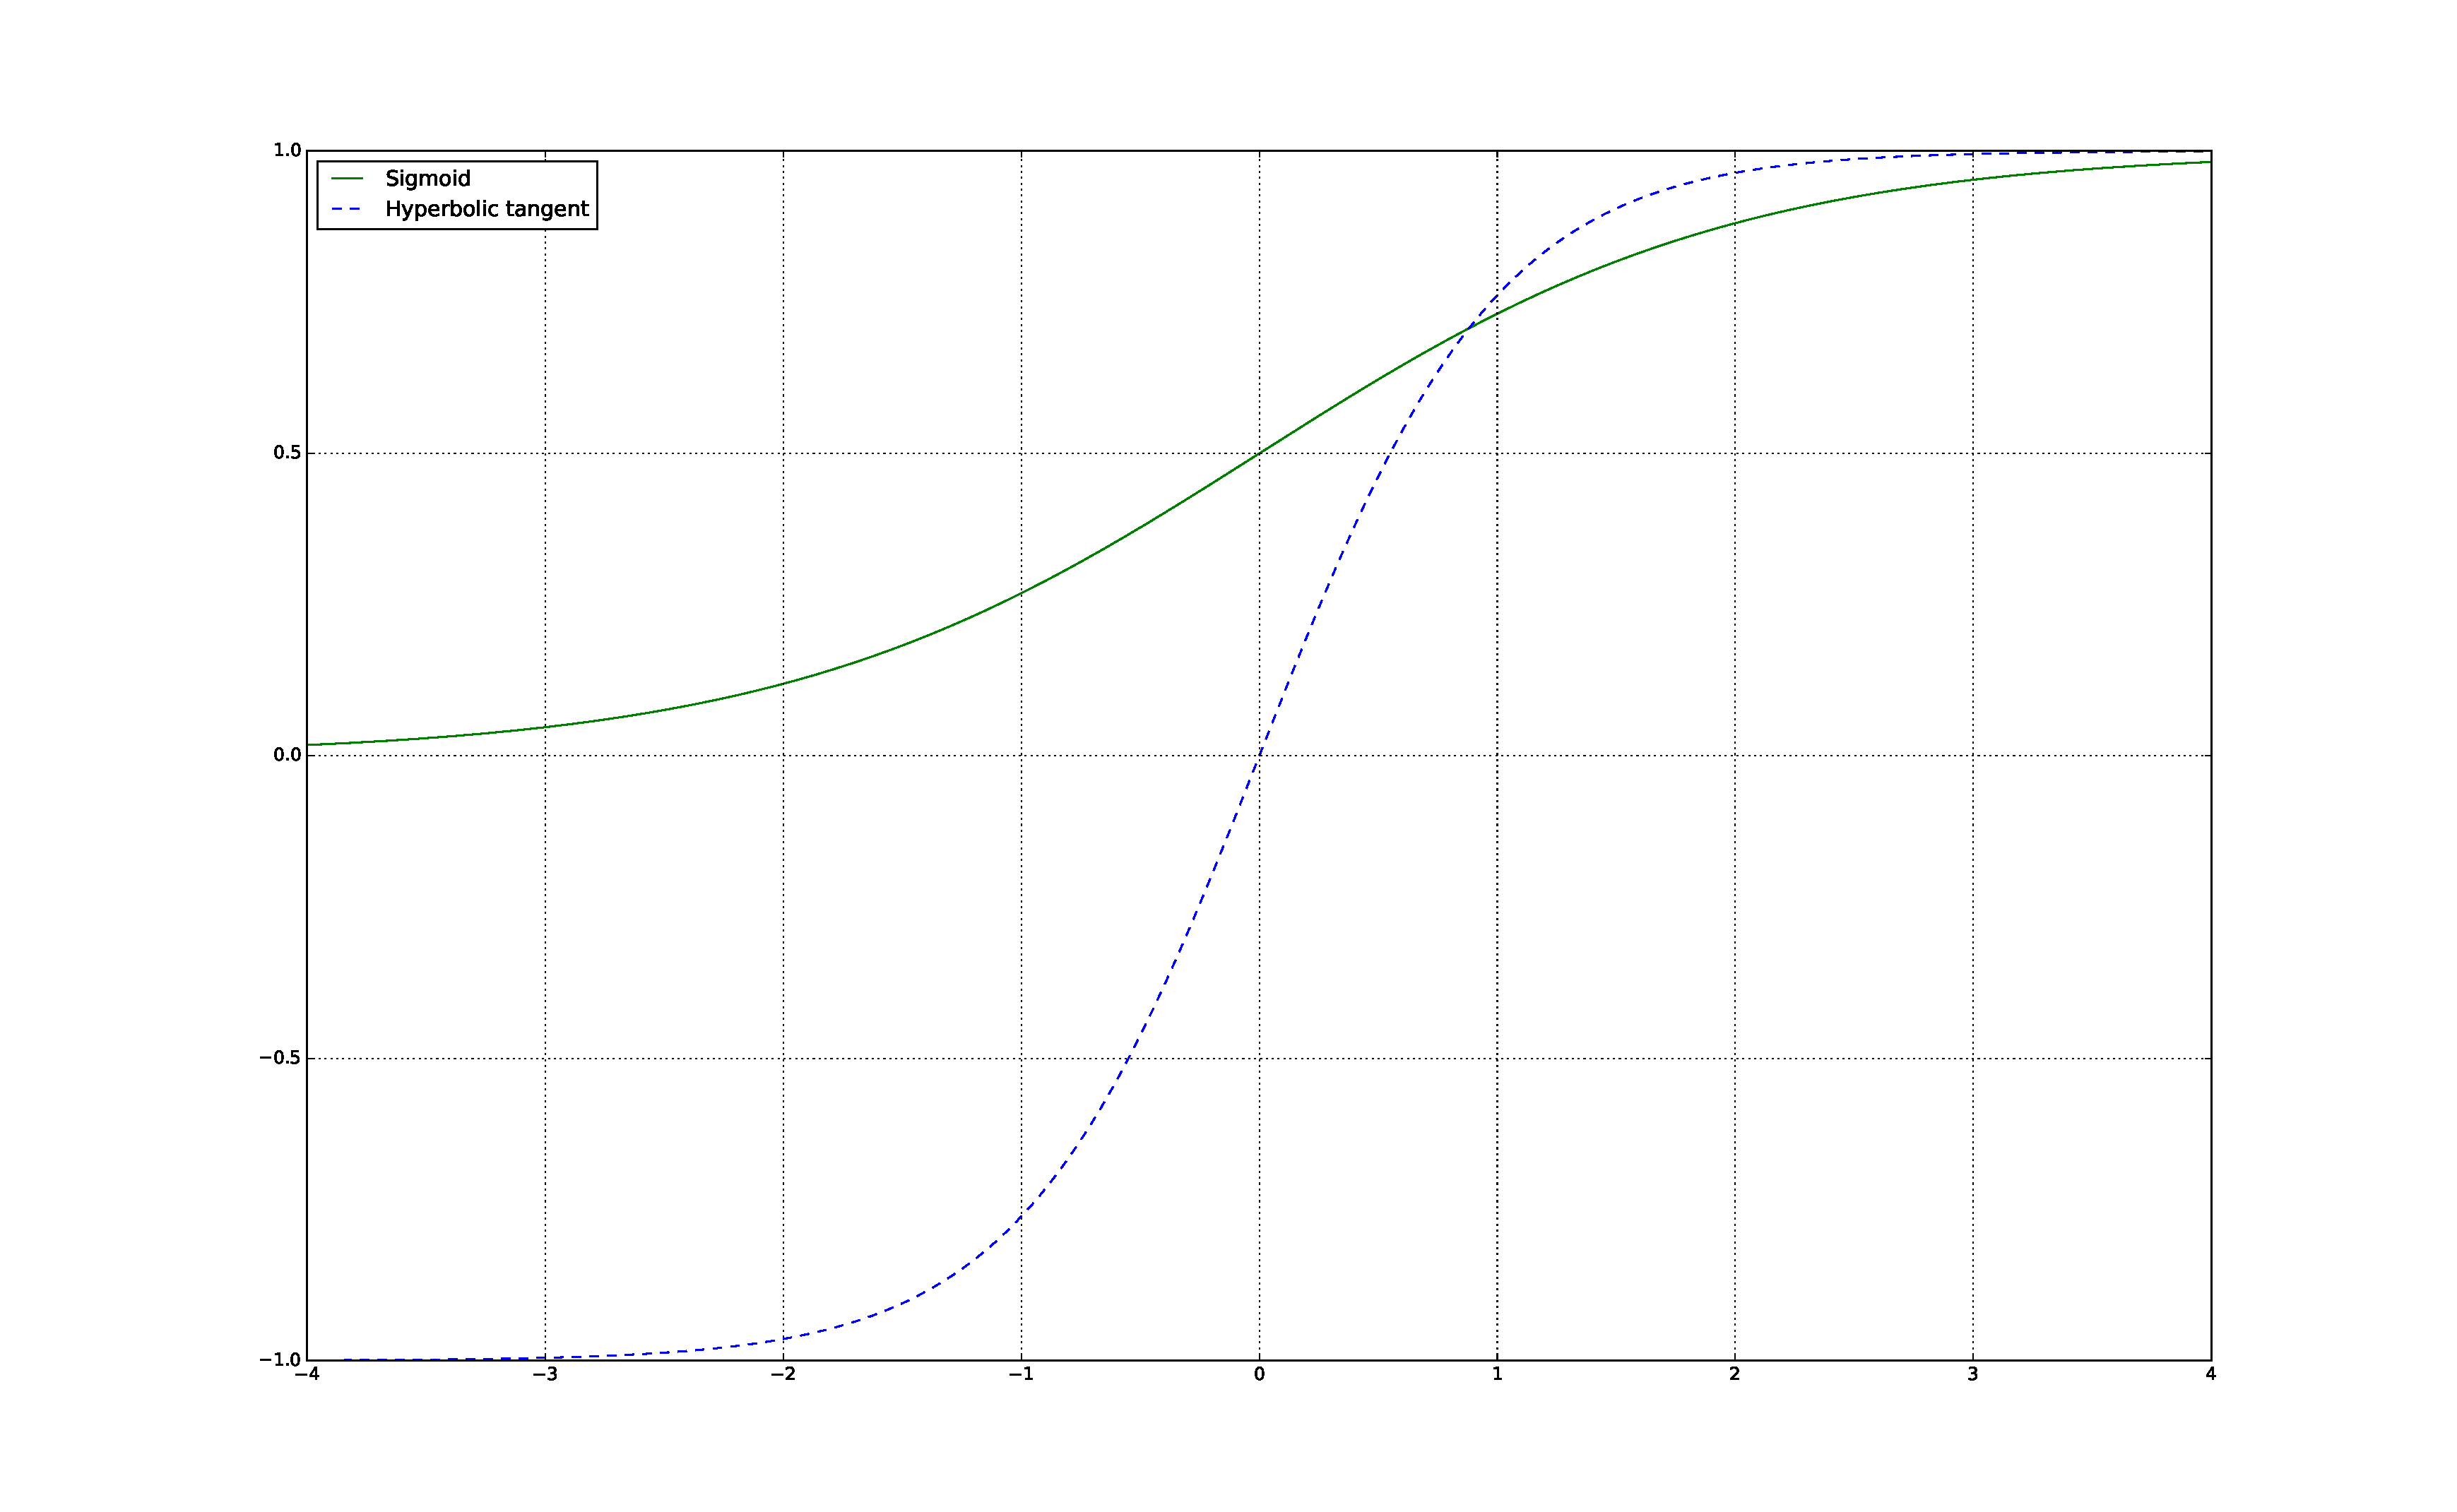
\includegraphics[width = 0.7\linewidth]{Figures/Theory/activationFunctions.pdf}
  \caption{Activation functions}
  \label{fig:activations}
  \end{center}
\end{figure}
Both these functions (Figure \ref{fig:activations}) have the desired properties mentioned above:
They are constant (1 or 0) for all values except a small interval around zero, where they have non-linear behaviour. 
This keeps the outputs of the neurons from blowing up. The sigmoid are more bilogically plausible because 
the output of inactive neurons are zero. Such activation function are called \textit{one-sided}. However,
it has been shown \cite{Karlik11} that the hyperbolic tangent 
performs better than the sigmoid for multi-layer networks. Nevertheless, one should assess the problem 
at hand when deciding what activation function to use; the performance can vary from problem to problem. 
(VENTE MED Å DISKUTERE DETTE TIL JEG HAR SNAKKET OM BACKPROPAGATION OSV.)
SNAKKE OM SATURATION OSV. 

In later years, the rectifier function (Figure \ref{fig:rectifier})
\begin{equation}
 f(x) = \max(0,x)
\end{equation}
has become the most popular for deep neural networks \cite{LeCun15}. PLOT DENNE FUNKSJONEN.
The two former functions are symmetrical around zero osv....
It have been argued to be even more biologically plausible than the sigmoid and also perform better
than the hyperbolic tangent for deep NNs. \cite{Glorot11}. 


A linear activation function $f(x) = x$ is often used in the output layer to avoid any constraint in the range 
of output values. For regression, the most widely used output activation is the unity function $f(x) = 1$, i.e.
no activation (HVORFOR?).

As shown in \eqref{completeNN}, the NN consists of several nested terms of the form
\begin{equation}
 h(x) = c_1 f(c_2 x + c_3) + c4
\end{equation}
where the parameters $c_i$ are weights and biases. By adjusting these parameters, the activation functions
can be shifted up and down or left and right, change slope or be rescaled, thus making the NN more flexible.

\subsection{Convolution}
ANNs are supposed to mimic biological systems. We know that neurons in the visual cortex of animals have
localized receptive fields, i.e. they respond only to stimuli in a certain location of the visual field. 
These regions are overlapping and covers the entire visual field. This can be exploited in ANNs by making the hidden layers
only connect to a small contigous region of the input layer. This also speeds up computations. These are called
locally connected networks, unlike fully connected networks, where all the hidden layers are connected to the complete
input layer. 

Using this approach, we can aggregate statistics of these features at various locations. This is called pooling. 

\section{Training}
The ability of the NN to represent a function accurately depends on the values of the weights. 
The weights are typically initialized as random numbers, and then optimized iteratively to minimize the error
to a set of expected output values. The expected output values are in our case known energies of a set of atomic
configurations, which have been obtained in quantum mechanical calculations of electronic structure. 
This optimization is called \textit{training} and an iteration is called an \textit{epoch}. 
The fitting process corresponds to the minimization of an error function, also known as the quadratic \textit{cost} function
\begin{equation}
 \Gamma = \frac{1}{2N}\sum_{i=1}^N (E_{i,ref} - E_{i,NN})^2
 \label{quadraticCostFunction}
\end{equation}
$E_{i,ref}$ are the known target energies, while $E_{i,NN}$ are the energies produced by the network. 
The constant $1/2$ are there to cancel out the exponent when we differentiate later. 
Other cost functions are used for other ML tasks (SKRIVE OM DISSE. KANSKJE HELE DENNE SEKSJONEN BØR 
SKRIVES MER GENERELL OG IKKE KUN FOR TILFELLET PES?)

\subsection{Backpropagation} \label{sec:backprop}
From: https://www.willamette.edu/~gorr/classes/cs449/backprop.html and \newline
http://neuralnetworksanddeeplearning.com/chap2.html. 
Mainly from the first one, but argument for error of neuron from second.

There are a large number of algorithms that can be used to determine the set of weights minimizing the 
cost function \eqref{quadraticCostFunction}. 
Different kinds of gradient descent methods are widely used, but to implement these we need the partial derivatives of
the cost function w.r.t. to all weights and biases to determine how we should adjust each weight. The idea behind gradient descent 
methods is to minimize a function by iteratively taking steps in the direction of the negative of its gradient w.r.t. 
all its parameters, i.e. the direction of steepest descent towards a minima:
\begin{equation}
 w_{ij}^{new} = w_{ij}^{old} - \gamma \frac{\partial \Gamma}{\partial w_{ij}^{old}}
 \label{gradientDescent}
\end{equation}
where we have skipped the layer indicies for clarity. Also, $w_{ij}$ now denotes the weight connecting node $j$ 
in layer $k$ with node $i$ in the following layer. This change of order is introduced to make it easier
to rewrite the below equations for backpropagation into matrix-vector equations. 
As seen from \eqref{gradientDescent}, we need to adjust each weight by an amount
\begin{equation}
\Delta w_{ij} = \frac{\partial \Gamma}{\partial w_{ij}}
\label{weightChange}
\end{equation}
The corresponding expression for the biases is
\begin{equation}
 \Delta b_i = \frac{\partial \Gamma}{\partial b_i}
\end{equation}
A common method to obtain these derivatives is backpropagation \cite{Rumelhart86}. 
In backpropagation, the output of the NN is compared to the desired output, the error is then propagated backwards
to adjust the weights. The method is essentially an implementation of the chain rule, and will allow us to calculate
the partial derivatives of the cost with respect to all the weights, thereby obtaining the gradient of the network. 

To change the value of the cost function \eqref{costFunction}, we need to change the outputs of the neurons in the network. 
Changing the input to neuron $j$ by a small amount $\Delta x_j$ results in the output
\begin{equation}
 y_j = f_j(x_j + \Delta x_j)
 \label{neuronError}
\end{equation}
This change will propagate through later layers in the network, finally causing the overall cost to change
by an amount $\frac{\partial \Gamma}{\partial x_j}\Delta x_j$. If $\partial \Gamma / \partial x_j$ is close to zero,
then we can't improve the cost much by perturbing the weighted input $x_j$; the neuron is already quite near the optimal value.
This is a heuristic argument for $\partial \Gamma / \partial x_j$ to be a measure of the error of the neuron:
\begin{equation}
 \delta_j \equiv \frac{\partial \Gamma}{\partial x_j}
\end{equation}
We also define
\begin{equation}
 A_i = \{j:w_{ij}\}
\end{equation}
as the set $\{j\}$ of nodes anterior to node $i$ and connected to node $i$ with weights $w_{ij}$, in addition to
\begin{equation}
 P_j = \{i:w_{ij}\}
\end{equation}
as the set $\{i\}$ of nodes posterior to node $j$ and connected to node $j$ with weights $w_{ij}$. 

The weight change \eqref{weightChange} can be expanded into two factors by use of the chain rule:
\begin{equation}
 \Delta w_{ij} = \frac{\partial \Gamma}{\partial x_i}\frac{\partial x_i}{\partial w_{ij}}
\end{equation}
Now we move in the opposite direction compared to the feed-forward function composition stage: First we differentiate the cost w.r.t 
neuron $i$'s input, then we differentiate the input w.r.t. weight $w_{ij}$ connecting neurons $j$ and $i$. The first term on the right
is the error $\delta_i$ of node $i$. The second is
\begin{equation}
 \frac{\partial x_i}{\partial w_{ij}} = \frac{\partial}{\partial w_{ij}} \sum_{m\in A_i} w_{im}y_m = y_j
\end{equation}
Putting the two together, we get
\begin{equation}
 \Delta w_{ij} = \delta_i y_j
\end{equation}
To compute this quantity, we thus need to know the output and the error for all nodes in the network. 
The outputs are as we have seen
\begin{equation}
 y_i = f_i(x_i) = f_i\left(\sum_{j\in A_i} w_{ij}y_j + b_i\right)
 \label{forwardProp}
\end{equation}
The error for output neuron $o$ is
\begin{equation}
 \delta_o = \frac{\partial \Gamma}{\partial x_o} = \frac{\partial \Gamma}{\partial y_o}\frac{\partial y_o}{\partial x_o}
          = (d_o - f_o(x_o)) \frac{\partial f_o(x_o)}{\partial x_o}
\end{equation}
When doing regression our output neurons will have the unity activation function, which means that the error is reduced to
\begin{equation}
 \delta_o = d_o  - y_o
\end{equation}
This error is then propagated backwards through the network. Each hidden neuron will have an error
\begin{equation}
 \delta_j = \frac{\partial \Gamma}{\partial x_j} = 
 \sum_{i\in P_j} \frac{\partial \Gamma}{\partial x_i}\frac{\partial x_i}{\partial y_j}\frac{\partial y_j}{\partial x_j}
 \label{errorTerms}
\end{equation}
The first term on the right is the error of node $i$. The second is the derivative of the net input of all posterior
nodes $\{i\}$ w.r.t. the output of node $j$:
\begin{equation}
 \frac{\partial x_i}{\partial y_j} = \frac{\partial}{y_j}\left(\sum_{m\in A_i} w_{im}y_m + b_i\right) = w_{ij}
\end{equation}
while the third is the derivative of node $j$'s activation function w.r.t. its net input:
\begin{equation}
 \frac{\partial y_j}{\partial x_j} = \frac{\partial f_j(x_j)}{\partial x_j} \equiv f_j^\prime (x_j)
\end{equation}
Putting all the pieces together we obtain
\begin{equation}
 \delta_j = f_j^\prime(x_j)\sum_{i\in P_j} \delta_i w_{ij}
 \label{backProp}
\end{equation}
The above expression requires that we know the errors of all the posterior nodes
of node $j$. As long as there are no cycles in the network, there is an ordering of nodes from the output back to the 
input that respects this condition. It is therefore valid only for feed-forward NNs.
The errors are propagated backwards through the whole NN until we reach the input nodes. By propagating the error
of only one ouput neuron, we thus obtain the errors of all the neurons at once. This is the strength of the backpropagation
algorithm. 
For the biases, we have
\begin{equation}
 \Delta b_j = \frac{\partial \Gamma}{\partial b_j} = \sum_{i\in P_j} \frac{\partial \Gamma}{\partial x_i}
	      \frac{\partial x_i}{\partial y_j} \frac{\partial y_j}{\partial x_j} \frac{\partial x_j}{\partial b_j}
\end{equation}
The only new term her is the last one:
\begin{equation}
 \frac{\partial x_j}{\partial b_j} = \frac{\partial}{\partial b_j}\left(\sum_{m\in A_j} w_{jm}y_m + b_j\right) = 1
\end{equation}
Consequentially, the update rule for the biases is simply the error of each neuron:
\begin{equation}
 \Delta b_j = \delta_j
\end{equation}
For fully-connected FFNNs we can easily rewrite these equations in matrix notation. In this notation, 
the biases, inputs, outputs and errors for all nodes in a layer are combined into vectors, while all weights from 
one layer to the next form a matrix $W_l$, where $l$ denotes the layer number. The inputs to all the nodes in 
layer $l$ can be written
\begin{equation*}
    \left(\begin{array}{c}
            x_1^l \\
            x_2^l \\
            x_3^l \\
          \end{array} \right)
 = \left(\begin{array}{c c c}
            w_{11} & w_{12} & w_{13} \\
            w_{21} & w_{22} & w_{23} \\
	    w_{31} & w_{32} & w_{33} \\
   \end{array} \right)
   \left(\begin{array}{c}
            y_1^k \\
            y_2^k \\
            y_3^k \\
         \end{array}\right)
 + \left(\begin{array}{c}
          b_1^l \\
          b_2^l \\
          b_3^l \\
         \end{array}\right)
\end{equation*}
so that equation \eqref{forwardProp} takes the form
\begin{equation}
\vec{y}_l = f_l(W_l\vec{y}_{l-1} + \vec{b}_l)
\end{equation}
Comparing equations \eqref{forwardProp} and \eqref{backProp}, we observe that 
\begin{equation}
 \sum_{j\in A_i}w_{ij} = \left(\sum_{i\in A_j}w_{ij}\right)^T
\end{equation}
i.e. the weight matrices used in backpropagation are the transpose of the matrices used in forward activation.
The complete backpropagation algorithm including forward activation then looks as follows:
\begin{enumerate}
 \item Initialize the input layer:
 \begin{equation}
  \vec{y}_0 = \vec{x}_0
 \end{equation}
 \item Propagate the activity forward: for $l = 1,2,\dots ,L$:
 \begin{equation}
  \vec{y}_l = f_l(W_l\vec{y}_{l-1} + \vec{b}_l)
 \end{equation}
 \item Calculate the error in the output layer:
 \begin{equation}
  \vec{\delta}_L = \vec{t} - \vec{y}_L
 \end{equation}
 \item Calculate the error: for $l = L-1, L-2, \dots ,1$:
 \begin{equation}
 \vec{\delta}_l = (W^T_{l+1}\vec{\delta}_{l+1}) \cdot f_l^\prime (\vec{x}_l)
 \end{equation}
 \item Update the weights and biases: 
 \begin{equation}
  \Delta W_l = \vec{\delta}_l \vec{y}_{l-1}^T, \quad \Delta \vec{b}_l = \vec{\delta}_l
 \end{equation}
\end{enumerate}


\chapter{Neural networks in molecular dynamics}
Following \cite{Behler15} and \cite{Behler11symmetry}.
All the dynamics of a molecular system is determined by the multidimensional potential-energy surface (PES), which
in general is a real-valued function depending on all atomic coordinates in the system. Using the Born-Oppenheimer approximation
(FORKLARE ELLER REFERERE), 
various quantum mechanical methods like Hartree-Fock and density functional theory (DFT) are available to directly calculate
the PES and forces for a given configuration. Calculating the energies for all relevant configurations of a system is
demanding and time-consuming, and only a limited number of energies can be computed and stored. 
Consequentially, during a \textit{ab inito} molecular dynamics (MD) simulations, the energies and forces for all configurations visited
are not available beforehand. In \textit{ab inito} MD, energies and forces are therefore calculated on-the-fly, typically using DFT.
This is however a very inefficient approach. A more efficient method is to construct an analytical PES to use in simulations, 
but this can only be done for very simple systems.

A solution to this problem is the introduction of approximate PESs, and there are two fundamental approaches. 
The most widely used and convential method is to replace the solution of the Schrödinger equation by a simplified
energy expression based on physical considerations and reasonable approximations. These functions are not obtained
by ab inito methods, but can in many cases be sufficiently accurate to be used in simulations (BØR HA EN EGEN SEKSJON
OM DE VANLIGSTE POTENSIALENE).

An alternative approach is to employ machine learning (ML) potentials that have no direct physical meaning. 
The aim of these purely mathematical functions is to fit an analytic expression to a set of reference data
obtained by quantum mechanical calulations. There are various methods (REFERENCES). 
ML potentials are particularly useful
\begin{itemize}
 \item if long MD simulations are required
 \item if many MD trajectories are needed
 \item if the systems are too large for the application of QM methods
\end{itemize}
Physical and ML potentials thus enables us to extend the time and length scales of MD simulations
beyond the realm of ab inito methods. 

Feed-forward neural networks (FFNN) have been demonstrated to be useful for the construction of PESs because
they are universal function approximators. There is no restriction in the accuracy that can be achieved when 
constructing neural network potentials (NNP). Unlike physical potentials, they are not restricted by any \textit{ad hoc}
functional form. NNPs offer a number of advantages for the construction of PESs:
\begin{itemize}
 \item Energies can be fitted to very high accuracy, leaving only
 the underlying error of the reference data
 \item Evaluation of NNPs require much less CPU time than QM methods
 \item The NNP expression is unbiased and generally applicable to all types of bonding
\end{itemize}
Still, there are disadvantages one should be aware of:
\begin{itemize}
 \item The evaluation of NNPs are notably slower compared to the use of classical force fields
 \item NNP expressions have no physical interpretation, and have very limited extrapolation capabilities
 \item NNPs are, for the time being, only applicable to systems containing only a few
 different chemical elements (but many atoms)
\end{itemize}

\section{High-dimensional NNPs}
The use of a single FFNN to represent complicated systems containing many atoms of different types is not possible for several reasons.
First of all, the deegrees of freedom (the number of weight parameters) will be very many, making the training and evaluation
of the network slow. Secondly, the NN has a symmetry problem. It does not take into account that exchanging two or more atoms
can lead to an energetically equivalent configuration. For example, exchanging the positions of both hydrogen atoms
in a water molecule will not alter the configuration energy. However, noting that all weights have numerically different values,
changing the order of the input coordinates to the NN will result in a different energy value. This problem can be solved
by a different choice of input coordinates, discussed below. The third problem in using a single FFNN is that it is 
only applicable to the system size that has been used during the training. If the NN has been trained with 5 inputs, 
it can not be used for a system containing any other number of atoms. 
\begin{figure}[H]
\begin{center}
  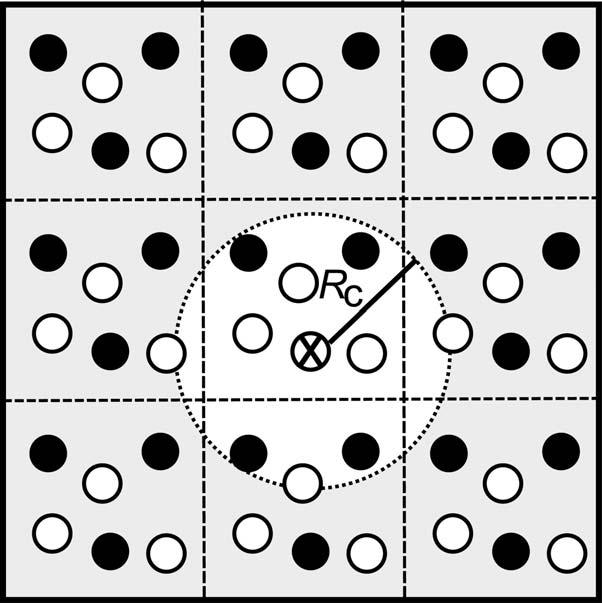
\includegraphics[width = 100mm]{Figures/Theory/cutOffHighDimNN.jpeg}
  \caption{}
  \label{fig:cutOffNeighbours}
  \end{center}
\end{figure}
A solution to all these problems is to construct the system energy $E_s$ as a sum of $N$ atomic energy contributions
$E_i$, which are provided by a set of individual atomic NNs,
\begin{equation}
 E_s = \sum_{i=1}^N E_i
 \label{systemEnergy}
\end{equation}
The atomic energies $E_i$ depend on the local chemical environment up to a cutoff radius $R_c$ as shown in figure
\ref{fig:cutOffNeighbours} (STJÅLET FRA PAPER, MÅ LAGE EGEN?). 
This is analogous to MD simulations with neighbour lists, thus making it possible to 
obtain the energies and forces of an atom and all its neighbours simultaneously. The positions of the neighbouring atoms within 
the cutoff sphere are described by a set of many-body symmetry functions discussed below. As the order of the summation does not 
change the total energy $E_s$, the symmetry problem above is solved. Each chemical element have seperate types of
NNs with their own architecture and weights, but for a given element all atomic NNs are equal. Such a system of NNs are also 
applicable to different system sizes: To add an atom of a given type, we simply extend the set of NNs by another network
identical to the other NNs of the same type, and if an atom is removed, we delete the respective NN. 
\begin{itemize}
 \item The introduction of the cutoff $R_c$ reduces the effective dimensionality
 of the problem, which allows to use NNs of tractable size
 \item The total energy is invariant with respect to the order of the atoms
 \item The NNP can be used for systems of different sizes
 \item We 
\end{itemize}
We know that the energy of a molcule does not change under a translation or a rotation. Thus our symmetry functions
should be invariant with respect to these operations. 

\subsection{Symmetry functions} \label{sec:symmetryFunctions}
To construct adequate symmetry functions, we need to have a cutoff function that defines the atomic environments. 
One such function is \cite{Behler15},
\begin{equation}
 f_c(R_{ij}) = 
\begin{cases}
0.5 \cdot \left[\cos\left(\frac{\pi R_{ij}}{R_c}\right) + 1 \right], & R_{ij} \leq R_c \\
0, & R_{ij} > R_c
\end{cases}
\label{cutoffFunction}
\end{equation}
which is the monotonically decreasing part of a cosine function on $R_{ij} \in [0,R_c]$, seen in \autoref{fig:cutoffFunction}. 
\begin{figure}[H]
\begin{center}
  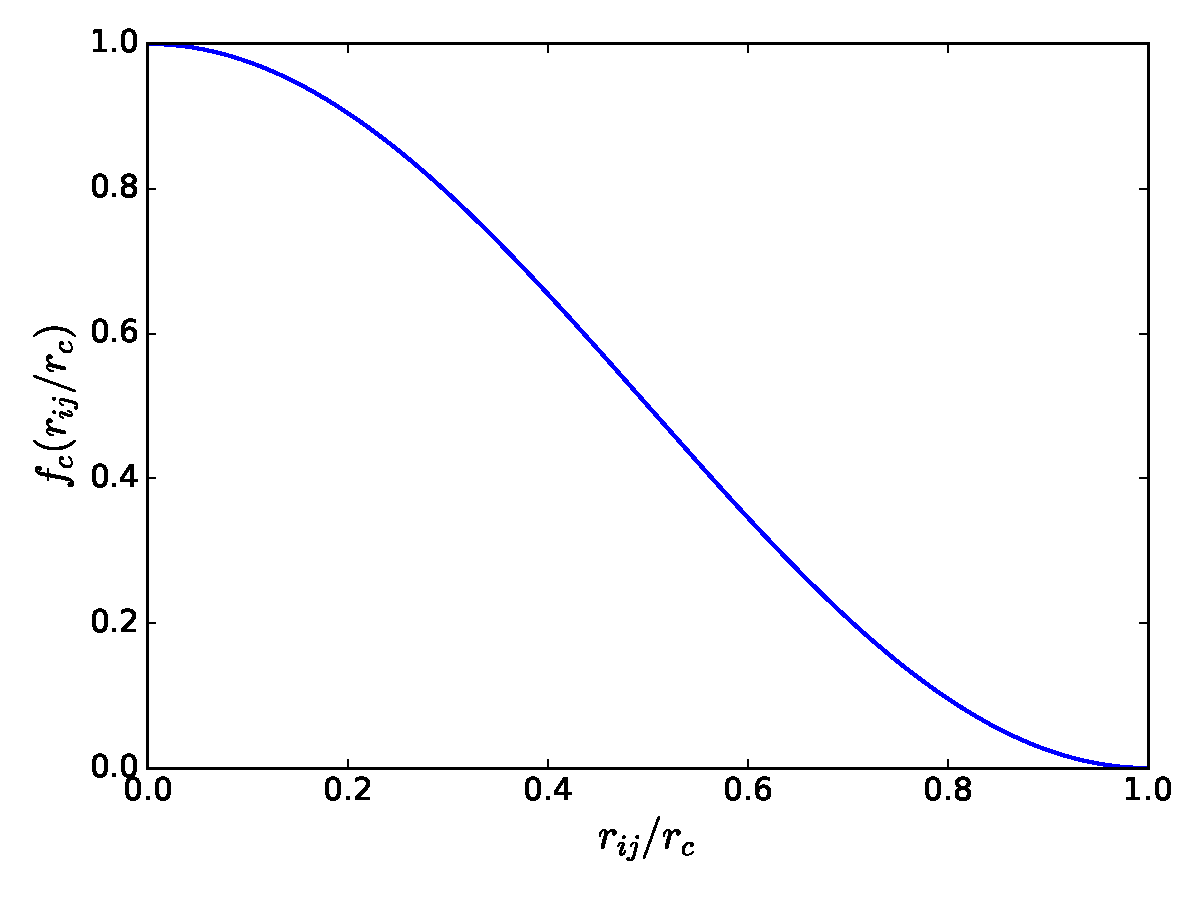
\includegraphics[width = 0.9\linewidth]{Figures/Theory/cutoffFunction.pdf}
  \caption{Plot of the cutoff function \eqref{cutoffFunction} applied in this thesis. 
	   This function is used to define a chemical environment around a central atom:
           only the atoms within the cutoff radius $R_c$ contribute to its energy. 
           These are called neighbouring atoms. The closer a neighbouring atom is, the larger
           the energy contribution, as is the case for most physical systems.}
  \label{fig:cutoffFunction}
  \end{center}
\end{figure}
This function have the desirable property that it decreases with increasing distance $R_{ij}$ between the central
atom $i$ and its neighbour $j$. At the cutoff radius $R_c$, is has zero value and slope, which is important
to avoid discontinuities when computing energies and forces. Atoms beyond the cutoff radius are not a part of the central
atom's chemical environment and therfore do not contribute to its energy. 

Several types of many-body symmetry functions can be
constructed based on these cutoff functions. They can be divided into two classes: \textit{radial} symmetry functions, describing 
the radial distribution of neighbours up to the cutoff radius, and \textit{angular} symmetry functions, specifying their
angular arrangement. All symmetry functions depend on the positions of all the atoms inside the cutoff spheres. They make
it possible to obtain a constant number of function values independent of the number of neighbours, which can change
during MD simulations. 

The most basic radial symmetry function is simply the sum of the cutoff functions for all the neighbours $j$ to 
atom $i$,
\begin{equation}
 G_i^1 = \sum_{j=1}^N f_c(R_{ij})
 \label{G1}
\end{equation}
We need a set of such functions with different cutoff radii to describe the radial arrangement of the neighbouring atoms. 
A better alternative is to use a sum of products of Gaussians and the cutoff function,
\begin{equation}
 G_i^2 = \sum_{j=1}^N \exp[-\eta(R_{ij}-R_s)^2] \cdot f_c(R_{ij})
 \label{G2}
\end{equation}
We now have two parameters that can be adjusted to probe different radii. The width parameter $\eta$ determines the 
radial extension of the symmetry functions, while the shifting parameter $R_s$ displaces the Gaussians to improve
the sensitivity of the symmetry functions at specific radii. A third option is 
\begin{equation}
 G_i^3 = \sum_{j=1}^N \cos(\kappa R_{ij}) \cdot f_c(R_{ij})
 \label{G3}
\end{equation}
which are damped cosine functions with a period length adjusted by parameter $\kappa$. We will however not use 
this function because of the existence of negative function values which can lead to atoms canceling each other's
contribution to the sum. In \autoref{fig:radialSymmetriFunctions} we see the radial symmetry functions for several
different parameters. It is clear that a set of such functions have a large flexibility when we tune the parameters
in different ways. This is what makes them able to represent the radial distribution of neighbours around a central atom. 
\begin{figure}[H] 
  \begin{subfigure}[b]{0.5\linewidth}
    \centering
    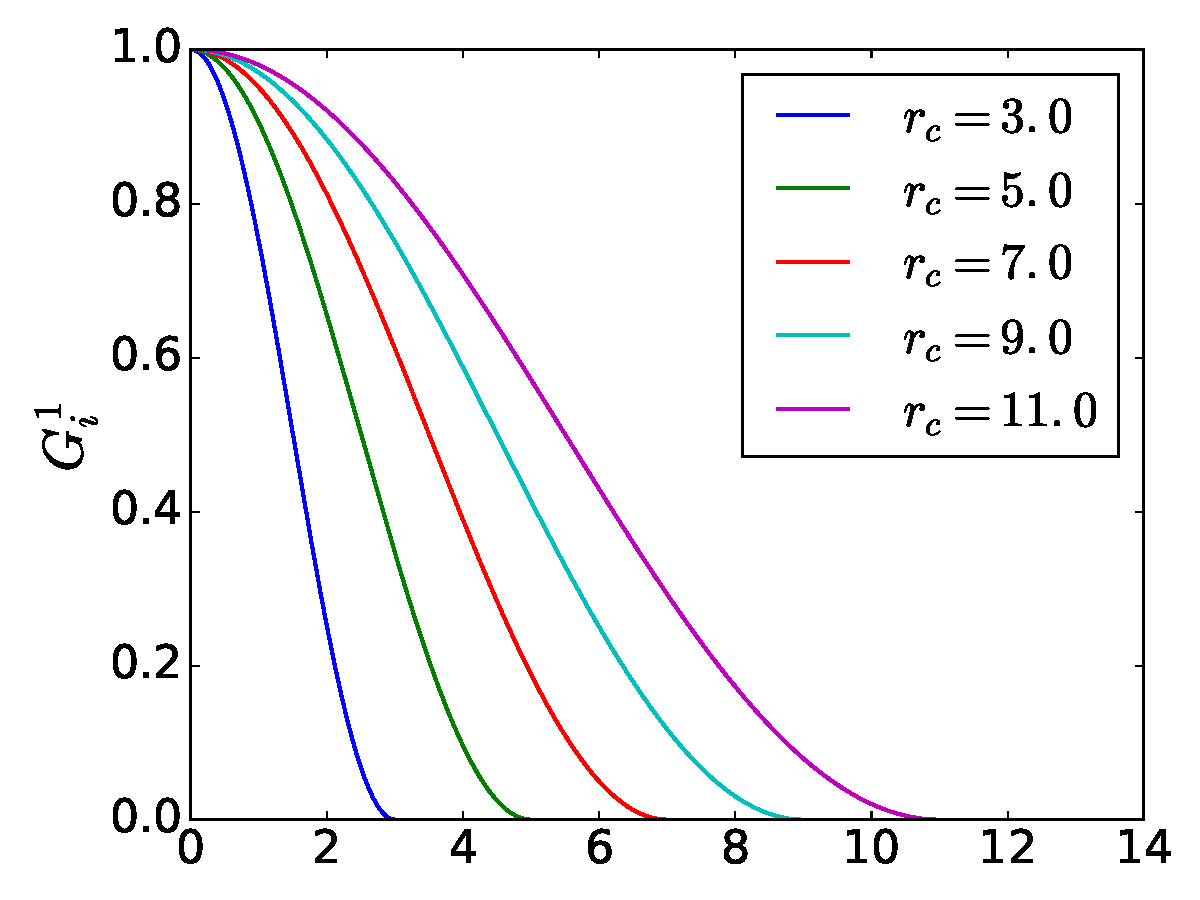
\includegraphics[width=\linewidth]{Figures/Theory/G1.pdf} 
    \label{fig:radialSymmetriFunctions:a} 
    \vspace{1ex}
  \end{subfigure}%% 
  \begin{subfigure}[b]{0.5\linewidth}
    \centering
    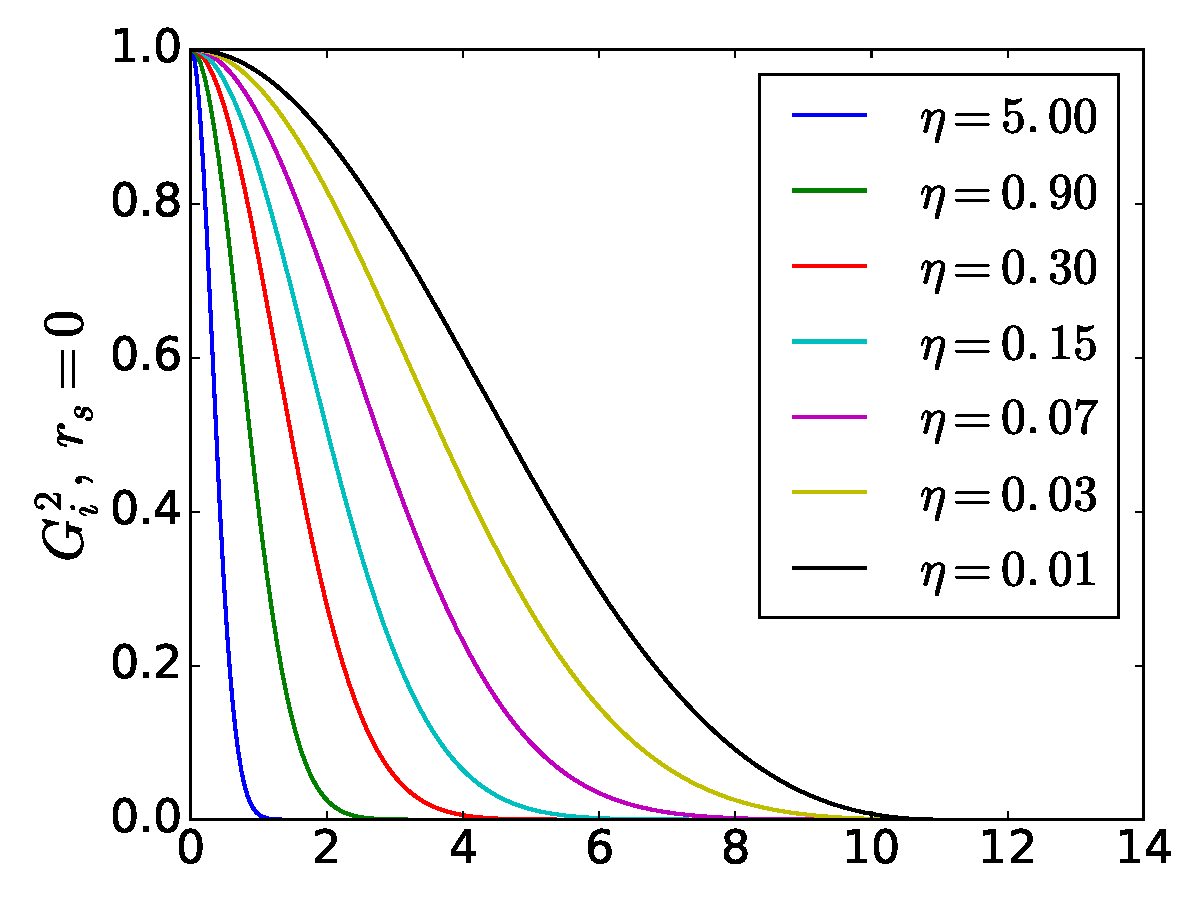
\includegraphics[width=\linewidth]{Figures/Theory/G2_1.pdf} 
    \label{fig:radialSymmetriFunctions:b} 
    \vspace{1ex}
  \end{subfigure} 
  \begin{subfigure}[b]{0.5\linewidth}
    \centering
    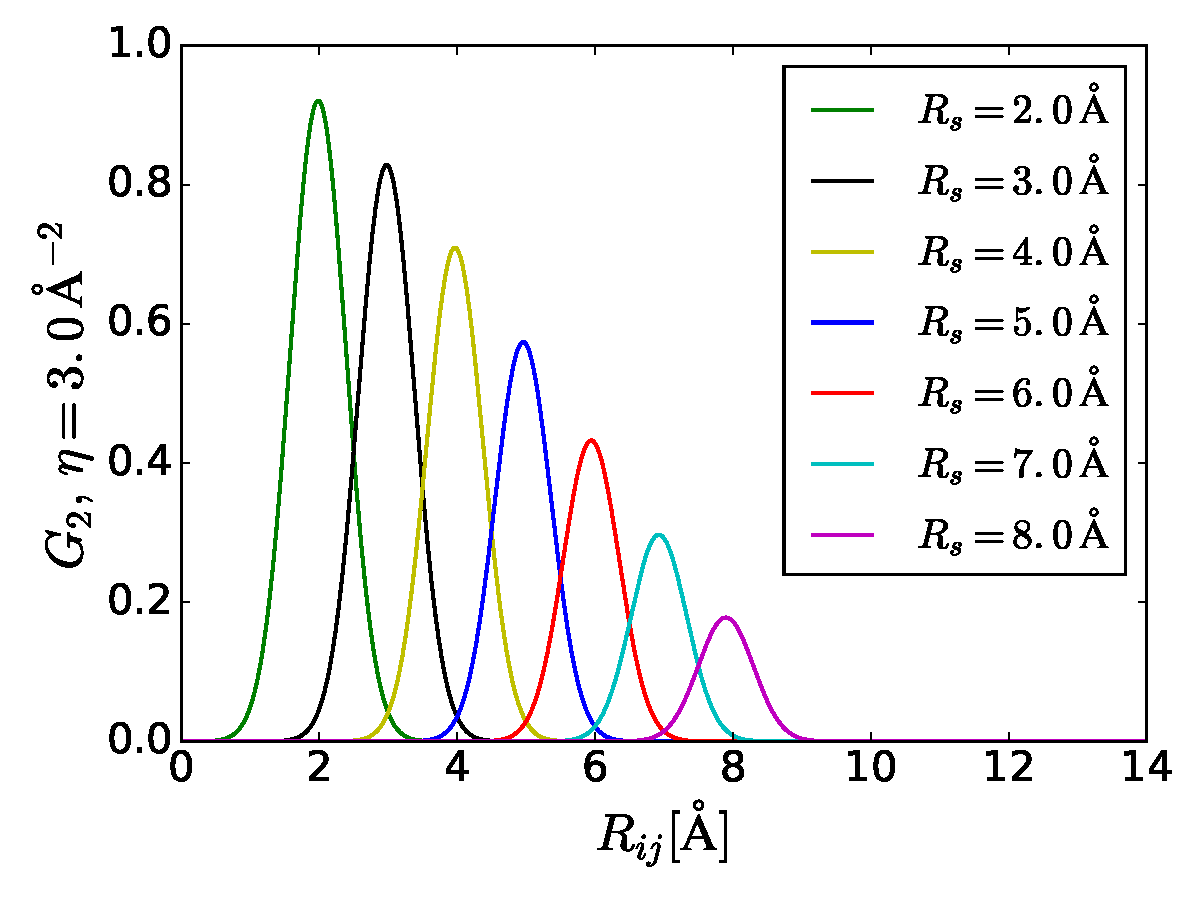
\includegraphics[width=\linewidth]{Figures/Theory/G2_2.pdf} 
    \label{fig:radialSymmetriFunctions:c} 
  \end{subfigure}%%
  \begin{subfigure}[b]{0.5\linewidth}
    \centering
    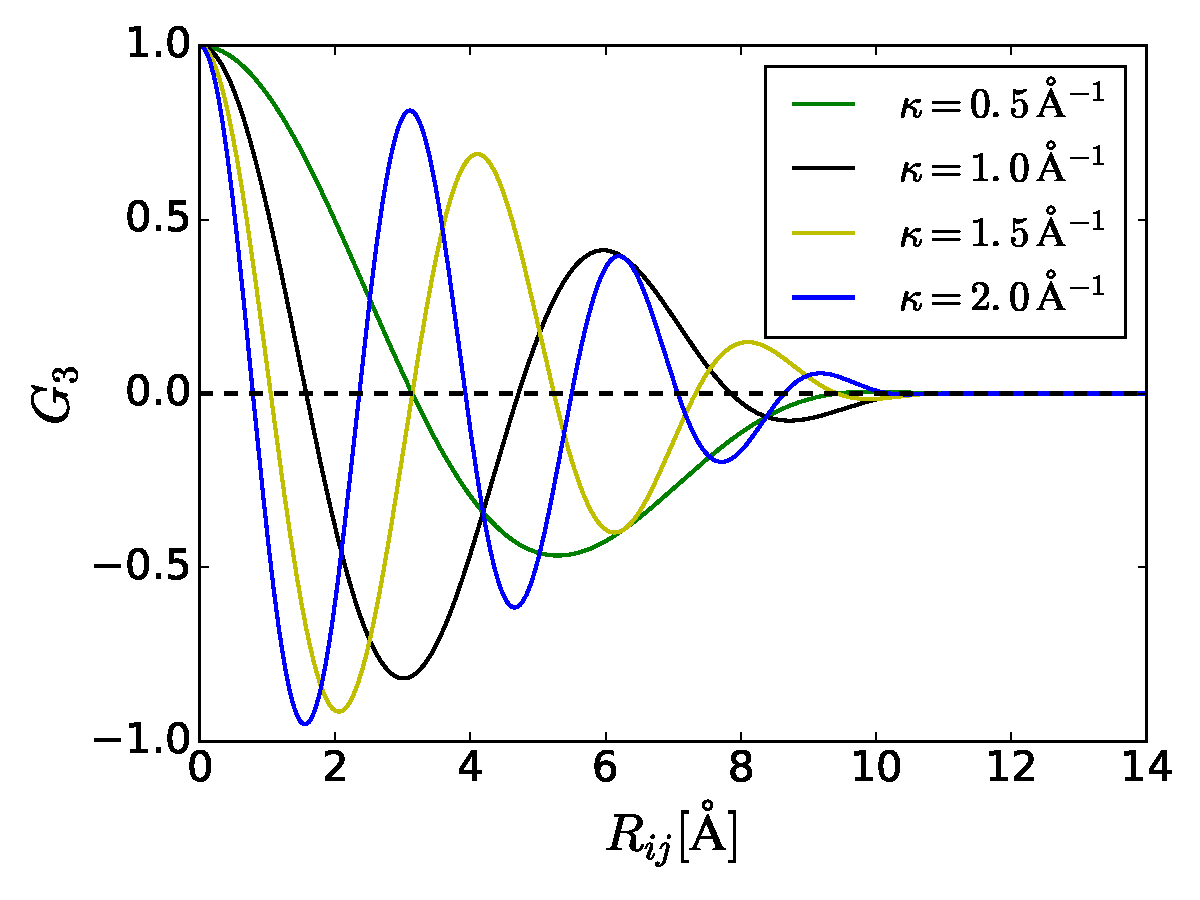
\includegraphics[width=\linewidth]{Figures/Theory/G3.pdf} 
    \label{fig:radialSymmetriFunctions:d} 
  \end{subfigure} 
  \caption{Radial symmetry functions $G^1$, $G^2$ and $G^3$ for an atom with one neighbour only. A set of such 
	   functions represents the radial distrubution of neighbours around a central atom placed at the origin.
	   For $G^2$ and $G^3$ a cutoff $R_c = \SI{11.0}{\angstrom}$ has been used.}
  \label{fig:radialSymmetriFunctions} 
\end{figure}
To obtain a suitable structural fingerprint of the atomic environments, we also need the angular distribution
of neighbouring atoms. This can be achieved by using functions depending on $\theta_{ijk}$, which
is the angle formed by the central atom $i$ and the two interatomic distances $R_{ij}$ and $R_{ik}$. 
The potential is periodic with respect to this angle, so we can use the cosine of $\theta_{ijk}$ instead. 
We thus define an angular symmetry function as a sum over all cosines with respect to any possible pair of 
neighbours $j$ and $k$, multiplied by Gaussians of the three interatomic distances and the respective cutoff functions,
\begin{align}
 G_i^4 = 2^{1-\zeta}\sum_{j\neq i}\sum_{k>j} &[(1 + \lambda \cos\theta_{ijk})^\zeta \cdot
 \exp(-\eta (R_{ij}^2 + R_{ik}^2 + R_{jk}^2)) \cdot \\
 &f_c(R_{ij}) f_c(R_{ik}) f_c (R_{jk})]
 \label{G4}
\end{align}
This function becomes zero if any of the interatomic distances is larger than $R_c$. The parameter $\eta$ takes here
into account that the angular contribution depends on the atomic seperations. The angular arrangement can be 
investigated by using different values for $\zeta$ while the normalization factor $2^{1-\zeta}$ ensures that the range of 
values is independent of the choice of $\zeta$. The parameter $\lambda \in {-1,1}$ can be used to invert the shape of the 
cosine function: for $\lambda = +1$ the maxima of the cosine terms are at $\theta_{ijk} = 0^\circ$, 
while for $\lambda=-1$ they are located at $\theta_{ijk} = 180^\circ$. The cutoff function $R_{jk}$
is included to ensure that only triplets where all three inter-atomic distances are within the cutoff radius. 
Another function can be defined that has no constraint on $R_{jk}$,
\begin{align}
  G_i^5 = 2^{1-\zeta}\sum_{j\neq i}\sum_{k>j} &[(1 + \lambda \cos\theta_{ijk})^\zeta \cdot
 \exp(-\eta (R_{ij}^2 + R_{ik}^2)) \cdot \\
 &f_c(R_{ij}) f_c(R_{ik})]
 \label{G5}
\end{align}
\eqref{G5} will generally have larger function values than \eqref{G4} because the lack of constraint on $R_{jk}$ results in 
a larger number of non-zero terms in the summation. The angular part of $G^4$ and $G^5$ is identical, shown in 
\autoref{fig:angularSymmetryFunctions} for different values of $\zeta$. 
\begin{figure}[H]
  \begin{subfigure}[b]{0.5\linewidth}
    \centering
    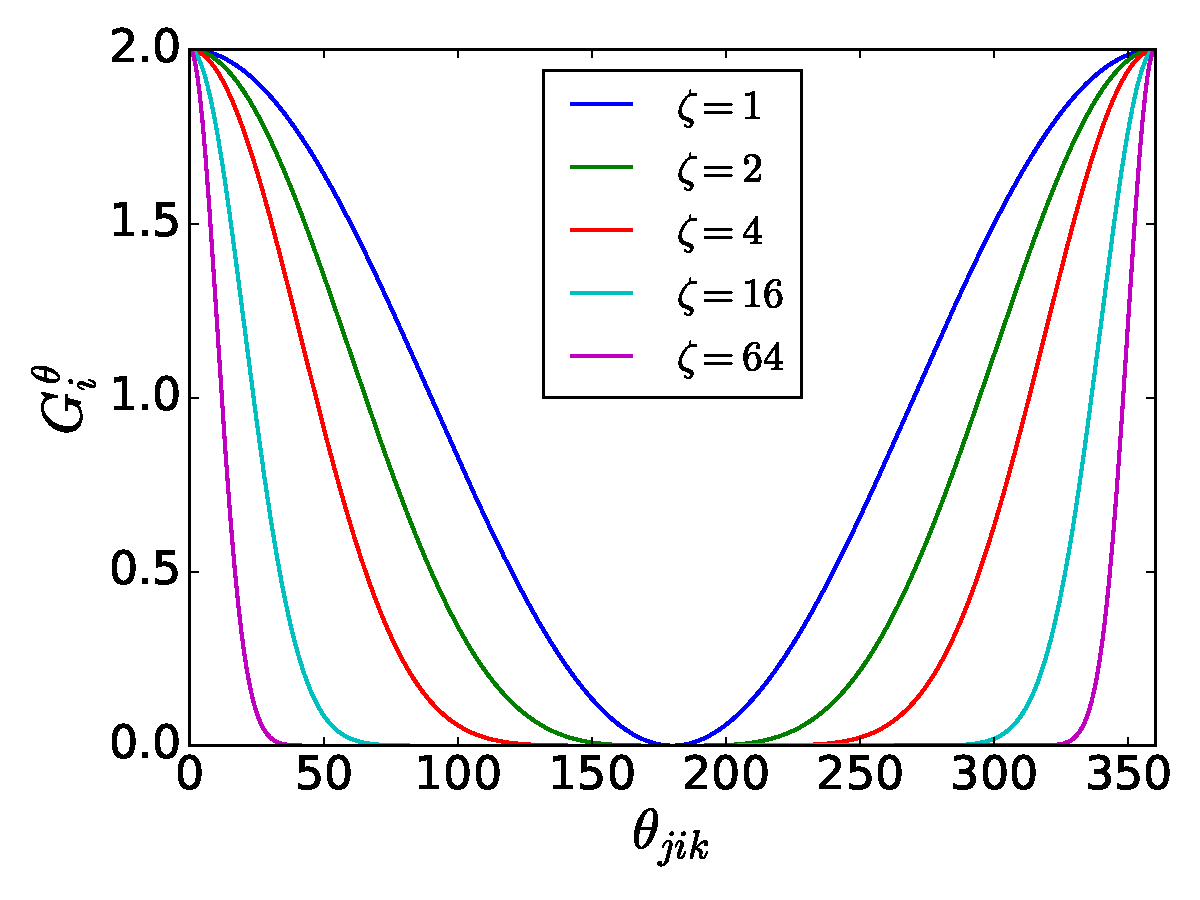
\includegraphics[width=\linewidth]{Figures/Theory/G4G5angular1.pdf}
    \subcaption{}
    \label{fig:angularSymmetryFunctions:a} 
  \end{subfigure}%% 
  \begin{subfigure}[b]{0.5\linewidth}
    \centering
    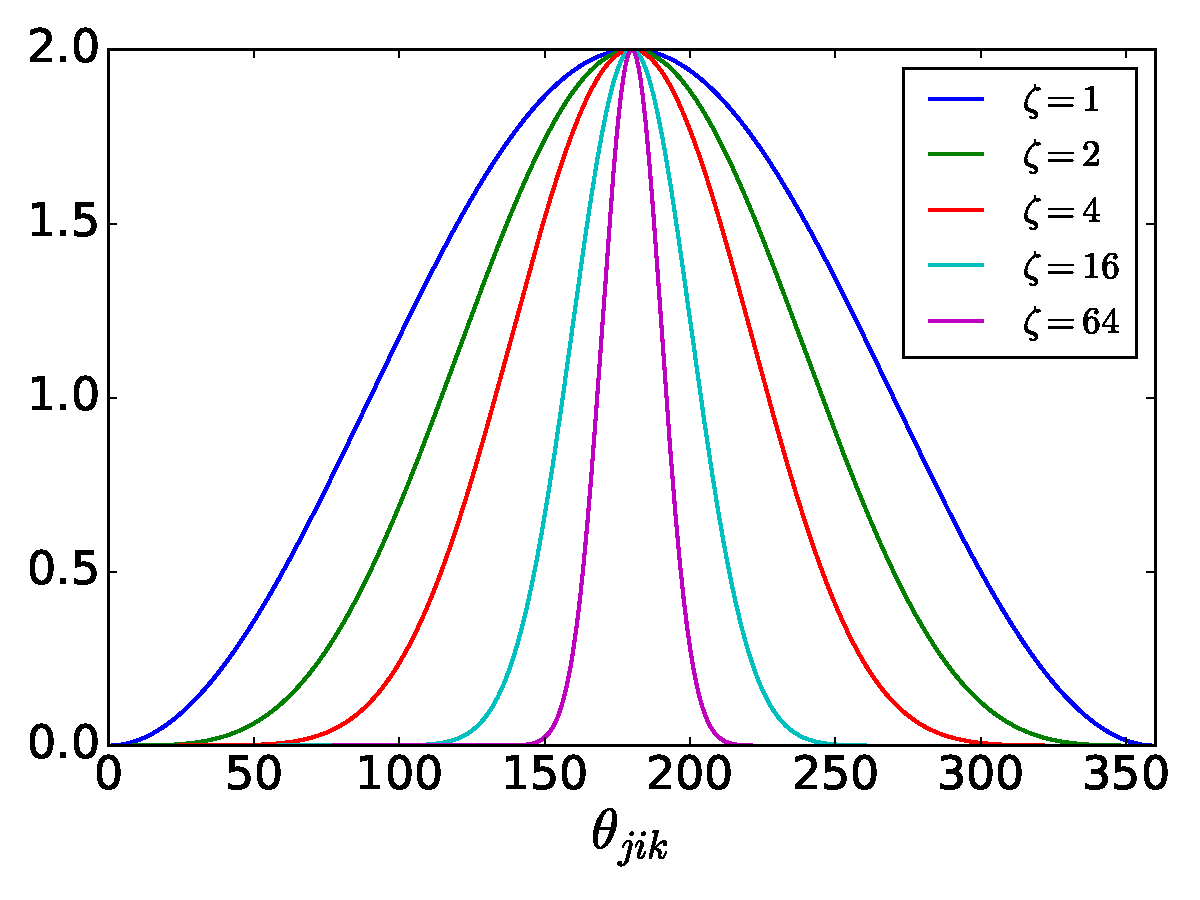
\includegraphics[width=\linewidth]{Figures/Theory/G4G5angular2.pdf} 
    \subcaption{}
    \label{fig:angularSymmetryFunctions:b} 
  \end{subfigure} 
  \caption{Angular part of symmetry functions $G^4$ and $G^5$ for an atom with one neighbour only. A set of such 
	   functions represents the angular distrubution of neighbours around a central atom placed at the origin.
	   $\lambda = +1$ for \autoref{fig:angularSymmetryFunctions:a}, $\lambda=-1$ for \autoref{fig:angularSymmetryFunctions:b}.}
 \label{fig:angularSymmetryFunctions} 
\end{figure}
The parameter values $R_c, \eta, R_s, \zeta$ and $\lambda$ are not automatically optimized, like the weights. 
Once a set of symmetry functions has been determined, they remain fixed during the training of the NN. They are therefore
an integral part of the NN, and need to be evaluated together with the NN itself when applied in simulations. 
The symmetry function set have to be customized for different systems, but in our experience the quality of the fit 
is not very sensitive to the choice of parameters. An adequate set will shorten the convergence time, but it will not 
necesseraly result in a lower RMSE. 
However, it is important to use at least as many symmetry functions as there are degrees of freedom in the system.
If this is not the case, the NN will recieve insufficient information and will not be able to fit the data properly. 

\subsection{Symmetry functions and forces}
To integrate Newton's laws in MD simulations we need the forces on all the atoms. The force field associated with a PES
was introduced in section \ref{sec:potentialEnergySurfaces} and is restated here for reference:
\begin{equation}
 \vec{F} = -\nabla E
 \label{forcePES2}
\end{equation}
In the present case, the total energy $E$ of the system is defined as a sum over all the atomic energies \eqref{systemEnergy}. 
Further, we have applied a cutoff so that each atom only gets energy contributions from its atomic environment up 
to a certain distance $R_c$.
The force component $F_{k,\alpha}$, $\alpha = (x,y,z)$ acting on atom $k$ with respect to coordinate $R_{k,\alpha}$,
can therefore be written \cite{Behler11symmetry}
\begin{equation}
 F_{k,\alpha} = -\frac{\partial E}{\partial R_{k,\alpha}} = -\sum_{i=1}^N\frac{\partial E_i}{\partial R_{k,\alpha}}
 = -\sum_{i=1}^{N_k+1}\frac{\partial E_i}{\partial R_{k,\alpha}}
 \label{forceAtomk}
\end{equation}
$N$ is as before the total number of atoms, while $N_k$ is the number of neighbours of atom $k$. 
Note that $E_k$ is included in the above sum - atom $k$ itself contributes to the total energy of its atomic
environment. We therefore have $N_k+1$ contributions. 

NNs have as we have seen well-defined functional forms, and analytical derivatives are therefore readily available.
However, when symmetry transformations is applied, there is only an indirect relation between the energy and the cartesian coordinates
of the atoms. To calculate the force \eqref{forceAtomk} we therefore need to apply the chain rule,
\begin{equation}
 F_{k,\alpha} = -\sum_{i=1}^{N_k+1}\frac{\partial E_i}{\partial R_{k,\alpha}} = 
 -\sum_{i=1}^{N_k+1}\sum_{s=1}^{M_i}\frac{\partial E_i}{\partial G_{i,s}}\frac{\partial G_{i,s}}{\partial R_{k,\alpha}}
 \label{forceAtomkChainRule}
\end{equation}
where $M_i$ is the number of symmetry functions of atom $i$. In other words, we need to sum over all the symmetry functions
of all the neighbours $i$ of atom $k$ and $k$ itself (IS THIS CORRECT???) Looking at Fiure (MAKE A FIGURE ILLUSTRATING
THE SYMMETRY TRANSFORMATION OF THE CARTESIAN COORDINATES THAT IS SENT TO THE NN), we realize that the first term
$\partial E_i\partial G_{i,s}$ is the derivative of the output of the atomic NN of atom $i$ with respect to the inputs,
i.e. the gradient of the NN. This is an analytical gradient
which is given by the architecture of the NN, including the values of the weights and biases.
We recall from \ref{sec:backprop} that the backpropagation algorithm calculates the derivatives of all neurons in a NN to obtain
the amount of which each weight and bias should be adjusted during training. We can thus use a slightly modified version
of this algorithm to compute the gradient of a NN,
\begin{enumerate}
 \item Instead of backpropagating the \textit{error} of the output neuron, 
 we backpropagate the \textit{derivative} of the output neuron's activation function.
 \item The derivative is propagated all the way back to the input nodes. During training, the propagation
 stops at the weights connecting the input layer and the first hidden layer. 
\end{enumerate}
This procedure clarifies how a fully-connected feed-forward NN is built: To get the derivative of the output neuron
w.r.t. the input neurons, we have to also compute the derivative of all the neurons in-between because
all nodes in each layer are connected to all nodes in the following layer. 

The second term $\partial G_{i,s}/\partial R_{k,\alpha}$ in \eqref{forceAtomkChainRule} is given by the 
definition of the employed symmetry functions. 
The derivatives of the Behler symmetry functions given in \autoref{sec:symmetryFunctions} are listed in \autoref{app:appendixA1}.
WRITE ABOUT DIFFERENTIATION WITH SYMPY AND TENSORFLOW ETC. 

In an MD simulation we only work with relative or inter-atomic coordinates and potentials. 
The training of neural networks is also based on an atom-centered approach; the cartesian coordinates
that is given as input to the symmetry functions are always atom-centered. This means that the atom
in question is placed at the origin and the positions of all neighbouring atoms are measured relative to 
the origin. Effectively, we are making a change of coordinates to the neighbours $\{j\}$ of the central atom $i$,
\begin{equation}
 \vec{r}_j \rightarrow \vec{r}_j - \vec{r}_i
 \label{changeOfCoordinates}
\end{equation}
This is in accordance with the Behler symmetry functions, which only operate with relative coordinates. 
It is however not trivial how this affects the above equations for the forces, which are not written in 
an atom-centered way. The process of obtaining the forces can be illustrated with an example system
consisting of three atoms of the same element with positions $\vec{r}_i$ where $i = 0,1,2$, shown in \autoref{threeAtoms}.
\begin{comment}\begin{figure}[H]
\begin{center}
  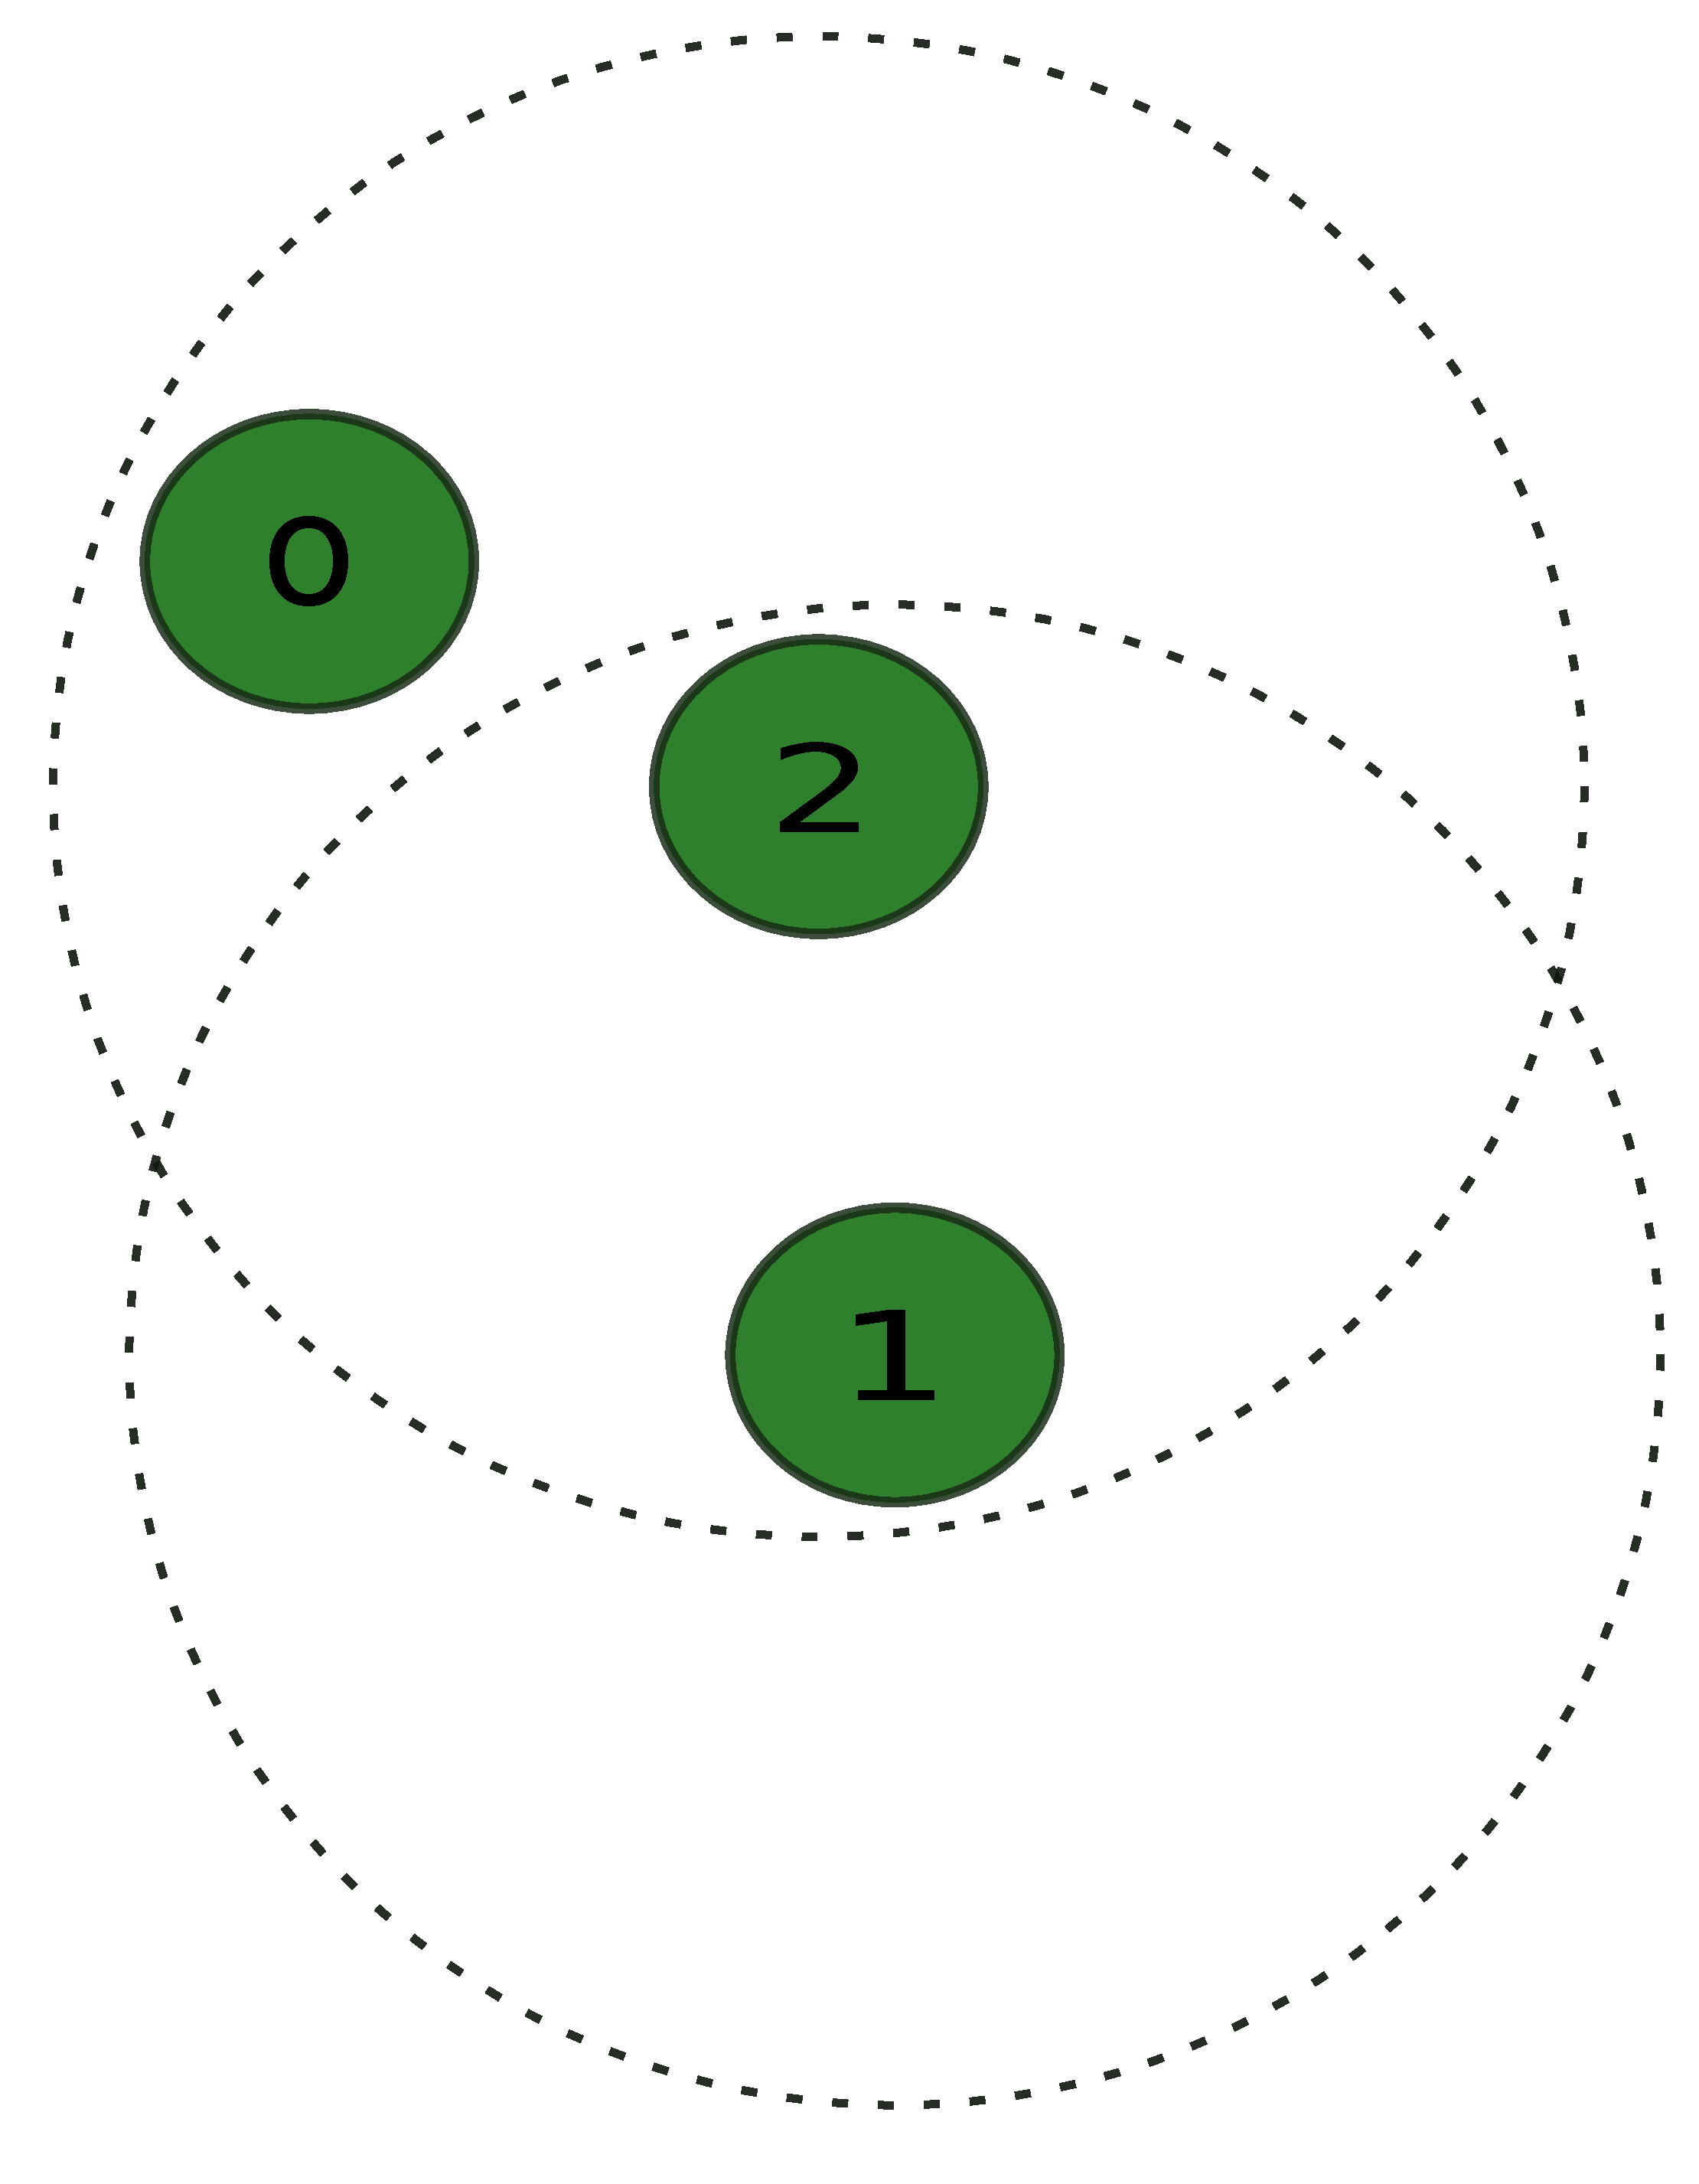
\includegraphics[width = 0.9\linewidth]{Figures/Implementation/3atoms.pdf}
  \caption{Example system of three atoms of the same type. Only atom 2 is inside the cutoff sphere of atom 1, thus we only need to 
	   take the energy of atom 1 and 2 into account to find the force on atom 1. Since the atoms are of the same type,
	   they have identical atomic NNs and symmetry function sets.}
  \label{fig:threeAtoms}
  \end{center}
\end{figure}\end{comment}
We want to find the force on atom 1 in the $x$-direction. Atom 0 is outside the cutoff sphere of atom 1, 
so according to \eqref{forceAtomk} the force is,
\begin{equation}
 F_{1,x} = \frac{\partial E_1}{\partial x_1} + \frac{\partial E_2}{\partial x_1}
\end{equation}
For simplicity, we assume that each atom only have two different symmetry functions describing their atomic environment;
one $G_{i,0}^2$ function describing the radial arrangement of neighbours and one $G_{i,1}^4$ dealing with the angular distribution.
Each atomic NN thus have two inputs and one output. 
Since the three atoms are all of the same type, they will have identical NNs and symmetry vectors. We will therefore 
denote the the two symmetry functions simply as $G^2$ and $G^4$. In the following we apply the notation
$r_{ij} = |\vec{r}_j - \vec{r}_i|$. 
The expressions for $E_1$ and $E_2$ then are,
\begin{equation}
 E_1 = \textrm{NN}\bigr[G^2(r_{10}) + G^4(r_{10},0,0)\bigr] = \textrm{NN}\bigr[G^2(r_{10})\bigr]
\end{equation}
where NN denotes the atomic neural network of the atoms. $G^4$ is zero because atom 1 only has one neighbour. Further, 
\begin{equation}
 E_2 = \textrm{NN}\bigr[G^2(r_{20}, r_{21}) + G^4(r_{20},r_{21},\theta_{021})\bigr]
\end{equation}
We note that atom 2 receives an energy contribution from both atom 0 and 1. 
To compute the derivatives of these energies with respect to the $x$-coordinate of atom 1, we
must take into account the change of coordinates \eqref{changeOfCoordinates}. We have that
\begin{equation}
 \frac{\partial G^n(x_{ij})}{\partial x_j} = \frac{\partial G^n(x_{ij})}{\partial x_{ij}}\frac{\partial x_{ij}}{\partial x_j}
 = \frac{\partial G^n(x_{ij})}{\partial x_{ij}}\frac{\partial (x_j-x_i)}{\partial x_j} = 
 \frac{\partial G^n(x_{ij})}{\partial x_{ij}}
 \label{changeOfCoordsSymmetry1}
\end{equation}
and
\begin{equation}
 \frac{\partial G^n(x_{ij})}{\partial x_i} = \frac{\partial G^n(x_{ij})}{\partial x_{ij}}\frac{\partial (x_j-x_i)}{\partial x_i} =
 -\frac{\partial G^n(x_{ij})}{\partial x_{ij}}
 \label{changeOfCoordsSymmetry2}
\end{equation}
This symmetry enables us to calculate the derivatives above. Applying the chain rule we get,
\begin{equation}
 \frac{\partial E_1}{\partial x_1} = \frac{\partial \textrm{NN}}{\partial G^2(r_{10})}
 \frac{\partial G^2(r_{10})}{\partial x_1} = 
 -\frac{\partial \textrm{NN}}{\partial G^2(r_{10})}\frac{\partial G^2(r_{10})}{\partial x_{10}}
\end{equation}
where we have applied the above change of coordinates \eqref{changeOfCoordsSymmetry1}.
Using \eqref{changeOfCoordsSymmetry2}, the derivative of $E_2$ can be calculated correspondingly,
\begin{align}
 \frac{\partial E_2}{\partial x_1} &= 
 \frac{\partial \textrm{NN}}{\partial G^2(r_{20}, r_{21})}\frac{\partial G^2(r_{20}, r_{21})}{\partial x_1} + 
 \frac{\partial \textrm{NN}}{\partial G^4(r_{20},r_{21},\theta_{021})}\frac{G^4(r_{20},r_{21},\theta_{021})}{\partial x_1} \\
 &= \frac{\partial \textrm{NN}}{\partial G^2(r_{20}, r_{21})}\frac{\partial G^2(r_{20}, r_{21})}{\partial x_{21}} + 
 \frac{\partial \textrm{NN}}{\partial G^4(r_{20},r_{21},\theta_{021})}\frac{G^4(r_{20},r_{21},\theta_{021})}{\partial x_{21}}
\end{align}
Based on these expressions we can do an observation that at first might seem strange. 
From the definition of $G_2$ \eqref{G2} we see that the sum contains two terms
in the case of atom 2, one for each pair interaction between atom 2 and its two neighbours. 
The interaction term between atom 0 and 2 will 
disappear when differentiated with respect to atom 1's coordinates, and is thus not included in the force on atom 1. 
The sum in $G_4$ \eqref{G4} however, consists of only one term corresponding to the only unique triplet with atom 2
as the central atom. This term is directly dependent on the coordinates of atom 0, which means that 
an atom which is outside the cutoff sphere of atom 1 still contributes to the force. This is an artefact of many-body potentials
like the NN potentials employed in this thesis: The force acting on an atom $i$ depends on the positions of the atoms as 
far as $2R_c$ away because neighbours $k$ of the neighbours $j$ of $i$ are included in the 
energies $E_j$ that is differentiated. 

This large effective range of atomic interactions is however not of great importance taking into account
that the interaction strength falls rapidly with distance for most systems where Coulomb forces are not included. 












\part{Implementation and validation}

\chapter{LAMMPS}
REFERENCE TO MANUAL - FOOTNOTE OF REFERNCE?
LAMMPS (Large-scale Atomic/Molecular Massively Parallel Simulator)
is a classical molecular dynamics simulation package 
developed at Sandia National Laboratories \cite{Plimpton95}. It is written
in highly portable and extendable objected-oriented c++. 
The package's functionality encompasses a wide variety of 
potentials, atom types, integrators, thermostats and 
ensembles and are able to simulate a large number
of different systems, including atoms, molecules, 
coarse-grained particles, polymers, graunular materials
and metals. LAMMPS can be run on a single processor
or in parallell. 
There exist several other molecular dynamics packages, 
like GROMACS, OpenMD, Aber and NAMD that could also
have served the purpose of this thesis. We have chosen
to work with LAMMPS because it is well documented, 
\footnote{\href{http://lammps.sandia.gov/doc/Manual.html}{http://lammps.sandia.gov/doc/Manual.html}}
easy to expand upon \footnote{\href{http://lammps.sandia.gov/doc/Developer.pdf}{http://lammps.sandia.gov/doc/Developer.pdf}}
and because the Computational
physics group at UiO has a lot of experience with using
it for molecular dynamics simulations. 
In this section we will outline the basic usage of LAMMPS, including
a walkthrough of an example input script. We also describe its
class hierarchy and how we can add our own functionality
to the package.

\subsection{Installing LAMMPS}
We have chosen to install LAMMPS by cloning
the Github repository and compile the source
code by running \texttt{make} in the source directory. 
To compile a serial version of the software, we simply run
the command
\begin{lstlisting}[language=bash]
 make serial
\end{lstlisting}
while the corresponding command for the parallel
MPI version is
\begin{lstlisting}[language=bash]
 make mpi
\end{lstlisting}
New updates can be downloaded by setting an
upstream git remote to point to the LAMMPS
GitHub repository and doing a \texttt{git fetch upstream}. 
LAMMPS also have several additional packages that
can be installed. This can be done by running
\begin{lstlisting}[language=bash]
 make yes-<package name>
\end{lstlisting}
e.g. \texttt{manybody} to install many-body potentials
like Stillinger-Weber and Vashishta. 

\subsection{LAMMPS input script}
LAMMPS is run by providing an input script as 
argument to the excecutable. This input script
is read line by line and has its own syntax. 
A good way to show the basics an input file
is to look at a simple example of a script
to measure diffusion in liquid argon,
\begin{lstlisting}[style=lammps]
# initialization
units 			metal		
dimension 		3
boundary		p p p		
atom_style		atomic		

# create geometry and atoms
lattice 		fcc 1.08506
variable		Nc equal 10
region 			myRegion block 0 ${Nc} 0 ${Nc} 0 ${Nc}
create_box		1 myRegion
create_atoms	1 box

# set mass and initial temperature
mass			1 1.0
variable		temp equal 300
velocity		all create ${temp} 87287 mom yes 

# compute diffusion
compute 		disp all displace/atom

# potential 
pair_style		lj/cut 2.5
pair_coeff		1 1 1.0 1.0 2.5
neighbor		0.5 bin
neigh_modify	every 20 delay 0 check no

# integration
timestep 		0.01
run_style 		verlet
fix 			integration all nve

# output
thermo			50
thermo_style 	custom step temp density press ke pe etotal 
thermo_modify 	norm yes

# run simulation
run				5000
dump 			diff all custom 100 diff*.dat c_disp[4]
run				10000
\end{lstlisting}
We will in the following briefly explain what
processes that are evoked in LAMMPS when the 
above commands are read. We start with the initialization of 
three basic properties of the simulation: units, boundary conditions and particle types.
\begin{lstlisting}[style=lammps]
 units 		metal
\end{lstlisting}
This command defines the units that are used 
in the simulation and the output. LAMMPS have eight
different unit sets. The \texttt{metal} set measures
distance in \AA{}ngstr\o{}m, energy in eV and temperature
in Kelvin. The choice of units depends on the system
that is investigated and the scale we are looking at.
\begin{lstlisting}[style=lammps]
 boundary 	p p p
\end{lstlisting}
We want to measure diffusion in a bulk
Argon liquid, thus we want to have periodic 
boundary conditions in all three dimensions, 
annotated by a \texttt{p}. LAMMPS can also handle stiff \texttt{f}
and adaptive \texttt{s} non-periodic boundaries. Adaptive
means that the position of the face is set so as to
encompass the atoms in that dimension. 
\begin{lstlisting}[style=lammps]
 atom_style atomic
\end{lstlisting}
Different systems need different information
to be stored for each atom. For style \texttt{atomic}, only
the default attributes are associated with each atom, 
namely coordinates, velocities, atom IDs and types. 
This is sufficient for pair-interacting, non-bonded
systems like Argon.

\noindent Next, we create the geometry of the simulation domain.
\begin{lstlisting}[style=lammps]
lattice 	fcc 5.720
\end{lstlisting}
This defines the initial configuration of the atoms. 
Here, a ffc lattice with a lattice constant of
5.720 is used. Other types of lattices based on
cubic or square unit cells are also available. 
\begin{lstlisting}[style=lammps]
variable	Nc equal 10
region 		simBox block 0 ${Nc} 0 ${Nc} 0 ${Nc}
\end{lstlisting}
The system's geometry is defined with the \texttt{region}
command. The \texttt{block} style is simply a 3-dimensional
straight-faced box with a size of $N_c = 10$ unit
cells in each dimension. We have labelled the 
region \texttt{simBox}. 
The number of unit cells
\texttt{N\_c} is defined as a LAMMPS \texttt{variable}. Variables
can be referenced elsewhere in the script by
writing \texttt{\$\{variable\_name\}} to become part of a new input
command like above. LAMMPS enables many styles
of variables to be defined. 
\begin{lstlisting}[style=lammps]
create_box		1 simBox
create_atoms	1 box
\end{lstlisting}
The command \texttt{create\_box} creates a simulation box 
based on the specified region, in our case the 
\texttt{block} region defined above. The argument specifies
the number of atom types that will be used in the
simulation. Next, \texttt{create\_atoms} with the argument
\texttt{box} fills the simulation
domain with atoms of type 1 on the lattice. 
LAMMPS also lets you create a random collection
of atoms or single atoms at specified coordinates.
\begin{lstlisting}[style=lammps]
mass			1 28
variable		temp equal 300
velocity		all create ${temp} 87287 
\end{lstlisting}
We need to assign mass to the atoms. For metal units, 
mass is measured in grams/mole. The atoms are also
given an initial velocity that corresponds to 
the given initial temperature. 
\begin{lstlisting}[style=lammps]
pair_style		lj/cut 2.5
pair_coeff		1 1 1.0 1.0 2.5
\end{lstlisting}
The choice of potential is made with the 
\texttt{pair\_style} command. We want to simulate
interactions using the cutoff Lennard-Jones potential
with a global cutoff of 2.5 Å. The LJ parameters
are set with \texttt{pair\_coeff}, the way this is done
depends on the potential being used. For our
choice of potential the arguments is as follows:
\texttt{atom-type-1 atom-type-2 sigma epsilon cutoff}. 
The parameters and cutoff can thus be set seperately 
for each pair of atom types.
\begin{lstlisting}[style=lammps]
neighbor		0.5 bin
neigh_modify	every 20 check yes
\end{lstlisting}
These commands sets parameters that affect the 
building of neighbor lists. The first argument
to \texttt{neighbor} is the skin size, while the 
second selects what algorithm is used
to build the lists. The \texttt{bin} style creates 
the lists by binning, which in most cases
(including ours) is the fastest method. 
Further, we can control how often the lists
are built with \texttt{neigh\_modify}. The above arguments
specifies that new neighbour lists are built 
every 20 steps, but every step LAMMPS checks
if any atom has moved more than half the skin distance.
If that is the case, new lists are built. 
\begin{lstlisting}[style=lammps]
timestep 		0.01
run_style 		verlet
fix 			integration all nve
\end{lstlisting}
LAMMPS integrates Newtons' equations of motion
with the velocity-Verlet algorithm by defualt. 
This is the integrator of choice for most MD
applications due to its simplicity and 
symplectic nature (REF TO SECTION). The 
rRESPA integrator \cite{Tuckerman92} scheme is also available.
LAMMPS does however not integrate and update
the positions and velocities of the particles
if not explicitly told so. This is done with
a \texttt{fix}, which is any operation that is applied to the 
system during timestepping. The above fix 
tells LAMMPS to integrate all atoms in the system 
so that they follow trajectories consistent with 
the microcanonical ensemble. 
\begin{lstlisting}[style=lammps]
thermo			50
thermo_style 	custom step temp press ke pe etotal 
thermo_modify 	norm yes
\end{lstlisting}
We can control what thermodynamic properties 
to calculate and output with \texttt{thermo\_style}, while 
\texttt{thermo} decides how often they should be computed. 
We want to output the time step, temperature, 
pressure, kinetic energy, potential energy and total
energy. Also, we want to normalize the extensive
quantities (the energies) by the number of atoms. 
\begin{lstlisting}[style=lammps]
 compute 		disp all displace/atom
 dump 			diff all custom 100 diff*.dat c_disp[4]
\end{lstlisting}
To measure diffusion in the 
Argon liquid, we need to calculate the net
displacement of all atoms. This can be done with a 
\texttt{compute}, which defines a computation that is 
performed on a group of atoms, in this case all atoms.
The \texttt{displace/atom} compute calculates the current
displacement of each atom from its original
coordinates, including all effects due to atoms
passing through periodic boundaries.
For the compute to actually be performed, it needs
to be evoked by other LAMMPS commands, like \texttt{dump}, 
which writes a snapshot of atom quantities to one 
or more files every N timesteps. Computes are 
referenced via the following notation \texttt{c\_ID}, where
ID is the ID of the compute. 
\begin{lstlisting}[style=lammps]
run		5000
\end{lstlisting}
Lastly, we run the simulation for 5000 timesteps. 
LAMMPS allowes several run commands to be issued
after one another. This comes in handy if we want
to thermalize the system before measuring diffusion.
This can be achieved by writing the following commands:
\begin{lstlisting}[style=lammps]
 run 	5000
 dump 	diff all custom 100 diff*.dat c_disp[4]
 run 	10000
\end{lstlisting}
When parsing the second run command, LAMMPS will
continue the dynamics while computing eventual
new fixes, computes, dumps etc. defined since
the last run command. 

This section has illuminated some of the basic
funcionality of LAMMPS through several comments
on a simple input script. Now we move on to
how class hierarchy of LAMMPS is structured. 

\subsection{LAMMPS structure}
LAMMPS is written in \texttt{C++} in an object-oriented
fashion. The class hierarchy is shown schematically
in figure (MAKE MY OWN FIGURE IN INKSCAPE). 
The blue classes are the core classes, these
are visible anywhere in LAMMPS.
Most of these have subclasses, of which the red ones
are called style classes. We recognize many 
of the input script commands among the style
classes; a rule of thumb is that every input script
command has a corresponding class and a
corresponding file name in the source directory. 
For instance, the cutoff Lennard-Jones potential
used in our input script is a subclass of Pair,
and is evoked by the command
\texttt{pair\_style lj/cut} and the source file is named
\texttt{pair\_lj\_cut}. 

We will not go into detail about the functionality
and communication of these classes. The one
that is the most relevant for this work is the \texttt{Pair} class. 
This is the parent class of non-bonded or pair-wise potentials, which
in LAMMPS includes many-body potentials like Stillinger-Weber and 
the Tersoff 3-body potential. The NN potential in this thesis falls 
under this category, and thus inherits from \texttt{Pair}. 
In the following section we will describe how 
LAMMPS can be extended with such a new \texttt{pair\_style}.

\subsection{Extending LAMMPS} \label{sec:extendingLammps}
To extend LAMMPS with a new component, we 
simply add a new \texttt{*.cpp} and \texttt{*.h} file to the 
source directory and re-compile. The new class
will (in theory) work with all other LAMMPS 
classes without breaking any functionality. 
A good strategy is to start with an existing potential
source file that is somewhat similar to the one 
we want to make, instead of programming from scratch.
We aim to construct a many-body non-bonded potential, and 
have chosen to base our implementation on the 
Stillinger-Weber potential file, \texttt{pair\_sw.cpp}.

The new potential class is added to LAMMPS with the following function call in the header file,
\begin{lstlisting}[language=c++]
 PairStyle(nn/manybody,PairNNManyBody)
\end{lstlisting}
The first argument is the name the potential will have in the input script, while 
the second is the name of the class. 
To use our new NN potential in a simulation we simply write,
\begin{lstlisting}[style=lammps]
 pair_style 	nn/manybody
\end{lstlisting}
in the input script. This command evokes two functions that need to be implemnted: \texttt{settings}
and \texttt{init\_style}. The former assures that no additional arguments are provided to 
\texttt{pair\_style} (I SHOULD MAYBE CHANGE THIS TO PROVIDE GLOBAL CUTOFF LATER???), while the latter
decides what kind of neighbour lists that LAMMPS should operate with. Our NN potential needs 
full neighbour lists to be able to compute three-body terms, something which applies to all many-body potentials. 

The parent class \texttt{Pair} has three \textit{pure virtual member functions}, i.e. functions that is required
to be implemented by a derived class: \texttt{compute}, \texttt{coeff} and the aforementioned \texttt{settings}. 
The \texttt{compute} method is where the forces and energies are calculated. This function is called
once each time step by the Verlet algorithm and the resulting forces are used to integrate Newton's equations
of motion. The coefficients of the employed potential are set in \texttt{coeff}, which in the case of a NN potential
is the weights and biases. These are read from file, and based on information on the architecture of the NN and 
choice of activation function, the network is reconstructed as a set of Armadillo matrices and 
vectors. This is achieved with the input script command,
\begin{lstlisting}[style=lammps]
 pair_coeff		* * <path-to-saved-NN> <cutoff> 
\end{lstlisting}
where the wildcard asterisks signify that the coefficients should be given to all pairs of atom types. 
THIS IS ONLY VALID FOR ONE ATOM TYPE. WRITE ABOUT MORE THAN ONE TYPE LATER. ALSO WRITE ABOUT
HOW THE ENERGIES AND FORCES ARE CALCULATED WHEN I HAVE TWO ATOM TYPES
UP AND RUNNING.





\chapter{TensorFlow}
TensorFlow \cite{Abadi15} \cite{Abadi16} is an open source software library 
developed by Google 
for numerical computation using data flow graphs (DFG). 
A DFG is a graphical representation of how data is
advanced through a system, including what kind of information is input
to and output from the system and where data is stored.
The data flow is represented as a directed graph
with a number of \textit{nodes} that is connected by
\textit{edges}. In TensorFlow, nodes represent
mathematical operations, while the edges represent
the multidimensional data arrays (tensors) 
communicated between them.

A simple example of a DFG is displayed in Figure (LAGE
EN FIGUR BASERT PÅ EKSEMPLET 
http://web.cecs.pdx.edu/~mperkows/temp/JULY/data-flow-graph.pdf
, which is a visualization of the flow of data
for the (real) solutions 
\begin{align}
 x_1 &= \frac{-b + \sqrt{b^2 - 4ac}}{2a} \\
 x_2 &= \frac{-b - \sqrt{b^2 - 4ac}}{2a}
 \label{quadraticEquationSolution}
\end{align}
of a quadratic equation
\begin{equation}
 ax^2 + bx + c = 0
\end{equation}
We observe that each node (circles)
contain the mathematical operations needed to compute
\eqref{quadraticEquationSolution}, while the arrows
(edges) show what data each node recieve and where
the output is sent. The inputs and outputs
of the computation is marked with rectangular
boxes. 

TensorFlow was originally developed by 
the Google Brain Team \footnote{\href
{https://research.google.com/teams/brain/}{https://research.google.com/teams/brain/}}
with the purpose of conducting machine learning and 
deep neural networks research, but is 
applicable in other domains as well, e.g. for
solving partial differential equations. 
The package incorporates
a wide variety of machine learning algorithms, including
convolutional neural networks and recurrent neural networks.
A computation expressed using TensorFlow can 
be executed on a wide variety of devices and systems, 
from mobile phones to large-scale distributed systems
and GPUs. 

In this chapter we will go through a simple 
example on how to build a computational graph 
with TensorFlow, and how to train a
feed-forward neural network. But first, a few
tips on how to install the software. 

\section{Installing TensorFlow}
The easiest way to install TensorFlow on Ubuntu
\footnote{\href{https://www.tensorflow.org/install/install\_linux}
{https://www.tensorflow.org/install/installlinux}}
(CHANGE LINK, IT IS WRONG BECAUSE OF UNDERSCORE...)
is to use pip, \footnote{\href{https://pip.pypa.io/en/stable/}
{https://pip.pypa.io/en/stable/}}
a package management system for software written in 
Python. Pip can be installed with the 
command
\begin{lstlisting}[language=bash]
 $ sudo apt-get install python-pip python-dev
\end{lstlisting}
TensorFlow can be installed with or without GPU 
support. The GPU version requires a system with
 CUDA-enabled NVIDIA GPUs
\footnote{\href{https://developer.nvidia.com/cuda-gpus}
{https://developer.nvidia.com/cuda-gpus}}. 
We have used the CPU version for the
development of our code, which is installed
with the command
\begin{lstlisting}[language=bash]
 $ pip install tensorflow
\end{lstlisting}
A simple
\begin{lstlisting}[language=bash]
 $ python -c "import tensorflow"
\end{lstlisting}
will test if the installation was succesful. 

\section{TensorFlow basic usage}
TensorFlow relies on highly-optimized
\texttt{C++} for its computations, but offers
APIs \footnote{\href{https://www.tensorflow.org/api_docs/}
{https://www.tensorflow.org/api\_docs/}}
in both \texttt{Python},
\texttt{C++} and a few other languages. 
The \texttt{Python} API is at present the most
complete, the easiest to use and the best documented.
We have therefore chosen to use \texttt{Python}
to train neural networks. For a discussion
on ways to import a trained NN to \texttt{C++} see
\autoref{sec:extendingLammps}
and \autoref{sec:timeUsage}. 

\subsection{Hello world}
As already mentioned, a TensorFlow computation
is described by a graph which consists of nodes
that communicate with multi-dimensional arrays along
interconnected edges. Each node has zero or more
outputs, and represents the instantation
of an \textit{operation}. Each operation
occurs within a so-called \textit{session}. 
A \texttt{Hello world!} program can be written as
\begin{lstlisting}[language=python]
import tensorflow as tf

hello = tf.constant('Hello world!')
sess = tf.Session()
print sess.run(hello)
# --> Hello world!
\end{lstlisting}
This simple example outlines the general
workflow for building a TensorFlow graph,
\begin{enumerate}
 \item Declare nodes (operations)
 \item Initiate a session
 \item Run operations within session
\end{enumerate}
The only operation in the above example
is the built-in TF constant that holds the 
\texttt{Hello world!} string, and the 
corresponding DFG only consists of one node. 
In more involved examples, visualizing 
the DFG can be useful for finding out how 
the script works. This is done with the 
included TF visualization tool TensorBoard.
We will now look at how to construct a neural network with TF and
visualize the corresponding DFG. 

\subsection{Creating a neural network}
In \autoref{sec:ANN} we saw how an artifical neural network could be written as a nested sum 
of activation functions \eqref{completeNN} where the weights connecting layer $l-1$ and $l$ were represented as
a matrix $W_l$, while the biases of layer $l$ were represented as a vector $\vec{b}_l$. The input vector $\vec{x}$ to 
the neurons in layer $l$, also called the \textit{preactivation}, can then be written
\begin{equation}
 \vec{x}_l = W_l \vec{y}_{l-1}  + \vec{b}_l
 \label{preActivationLayer}
\end{equation}
where $\vec{y}$ is the output vector of layer $l-1$. The activations of layer $l$ is thus
\begin{equation}
 \vec{y}_l = f(\vec{x})
 \label{activationLayer}
\end{equation}
where $f$ is the chosen activation function. This demonstrates that a NN can be constructed 
as a set of matrix-vector multiplications and additions which are input to a chosen activation function. 
We now want to construct a NN with 3 inputs neurons, one hidden layer with 10 neurons and 1 output neuron. 
We use the sigmoid \eqref{sigmoidActivationFunction} activation function for the hidden layer, while 
the output layer have the linear activation function (REF).
This can be achieved with the following \texttt{python} script,
\lstinputlisting[language=Python]{Scripts/TensorFlow/networkExample.py}
There are several aspects of the TensorFlow \texttt{python} API to comment on here. 
We observe that the input layer is declared as a TF \texttt{placeholder}. This is a special
type of TF tensor that is not initialized with any values, but is rather fed with data on its execution.
Specifying the first component of its shape as \texttt{None} signifies that we can supply an arbitrary 
number of data points at the same time.
These properties enables the same NN to be evaluated for different data vectors of varying size on-the-fly during training, 
explained in more detail below. 

The weights and biases are declared as TF \texttt{Variables}. These are the trainable parameters 
of the computational graph, and are normally constructed as random numbers. In the present case,
the weights are normally distributed numbers while the biases are all set to the same value 0.1. 
We note that the shapes of the weight matrices and bias vectors depend on the number of nodes in each layer.
If $n_l$ stands for the number of neurons in layer $l$, we have in general that the weight matrix connecting
layer $l-1$ and $l$ is of shape $n_{l-1} \times n_l$, while the bias vector of layer $l$ has $n_l$ number of elements. 

The activations (outputs) of each layer are calculated according to \eqref{preActivationLayer} and \eqref{activationLayer}. 
Together with the input \texttt{placeholder}, these are of type \texttt{tf.Tensor}, i.e. nodes in the computational 
graph. 

\subsection{Visualizing the graph}
We can use TensorBoard to visualize the DFG of the above script. The DFG for the present example is quite
simple, but for more involved models it quickly becomes difficult to keep track of all the different components. 
A convenient tool to order and group the DFG is \textit{name scoping}. Both \texttt{Tensors} and \texttt{Variables} can 
be name scoped and TensorBoard uses this information to define a hierarchy of the nodes in the graph. 
An example of name scoping is
\begin{lstlisting}[language=python]
 with tf.name_scope('layer1'):
    W1 = tf.Variable( tf.random_normal([inputs,nodes]), name='weights')
    b1 = tf.Variable( tf.constant(0.1, shape=[nodes]), name='biases')
\end{lstlisting}
which results in the following names,
\begin{itemize}
 \item \texttt{layer1/weights}
 \item \texttt{layer1/biases}
\end{itemize}
Additionally, TensorBoard will group the two variables together under \texttt{layer1}. 
To save the graph to file we have to start a TF session. The following script 
deploys name scoping, initiates a session and writes the DFG to file,
\lstinputlisting[language=python]{Scripts/TensorFlow/tensorBoardExample.py}\label{lst:tensorBoardExample}
There are two new TF function calls to comment on in this script. First, we have the line
\begin{lstlisting}[language=Python]
 initOperation = tf.global_variables_initializer()
\end{lstlisting}
Constants are initalized when we call \texttt{tf.constant}, and their value can never change. 
By contrast, variables need to be initialized using a seperate operation within a session. 
The function \texttt{tf.global\_variables\_initializer} adds such an operation to the graph, which initializes
all global variables when run with \texttt{sess.run(initOperation)}. 

Secondly, the graph is written to file for visualization with the function \texttt{tf.summary.FileWriter}. 
The first argument is the location of the files, while the second is the graph that is launched in the
present session. 

The resulting graph is displayed in \autoref{fig:graphExample}. 
By default, only the top of the hierarchy defined by name scoping is shown. In our case, this
is the three NN layers. In this figure, the output layer is expanded to reveal all the nodes in this scope. 
The nodes are marked by ellipses, while the rectangles are namespaces defining another level in the hierarchy, 
each containing more nodes. The edges show how the nodes are connected. 
\footnote{Each TF variable and constant are actually made up of several nodes, including \textit{assign} and 
\textit{read} operations. See TF API for more information.}
\begin{figure}[H]
\centering
  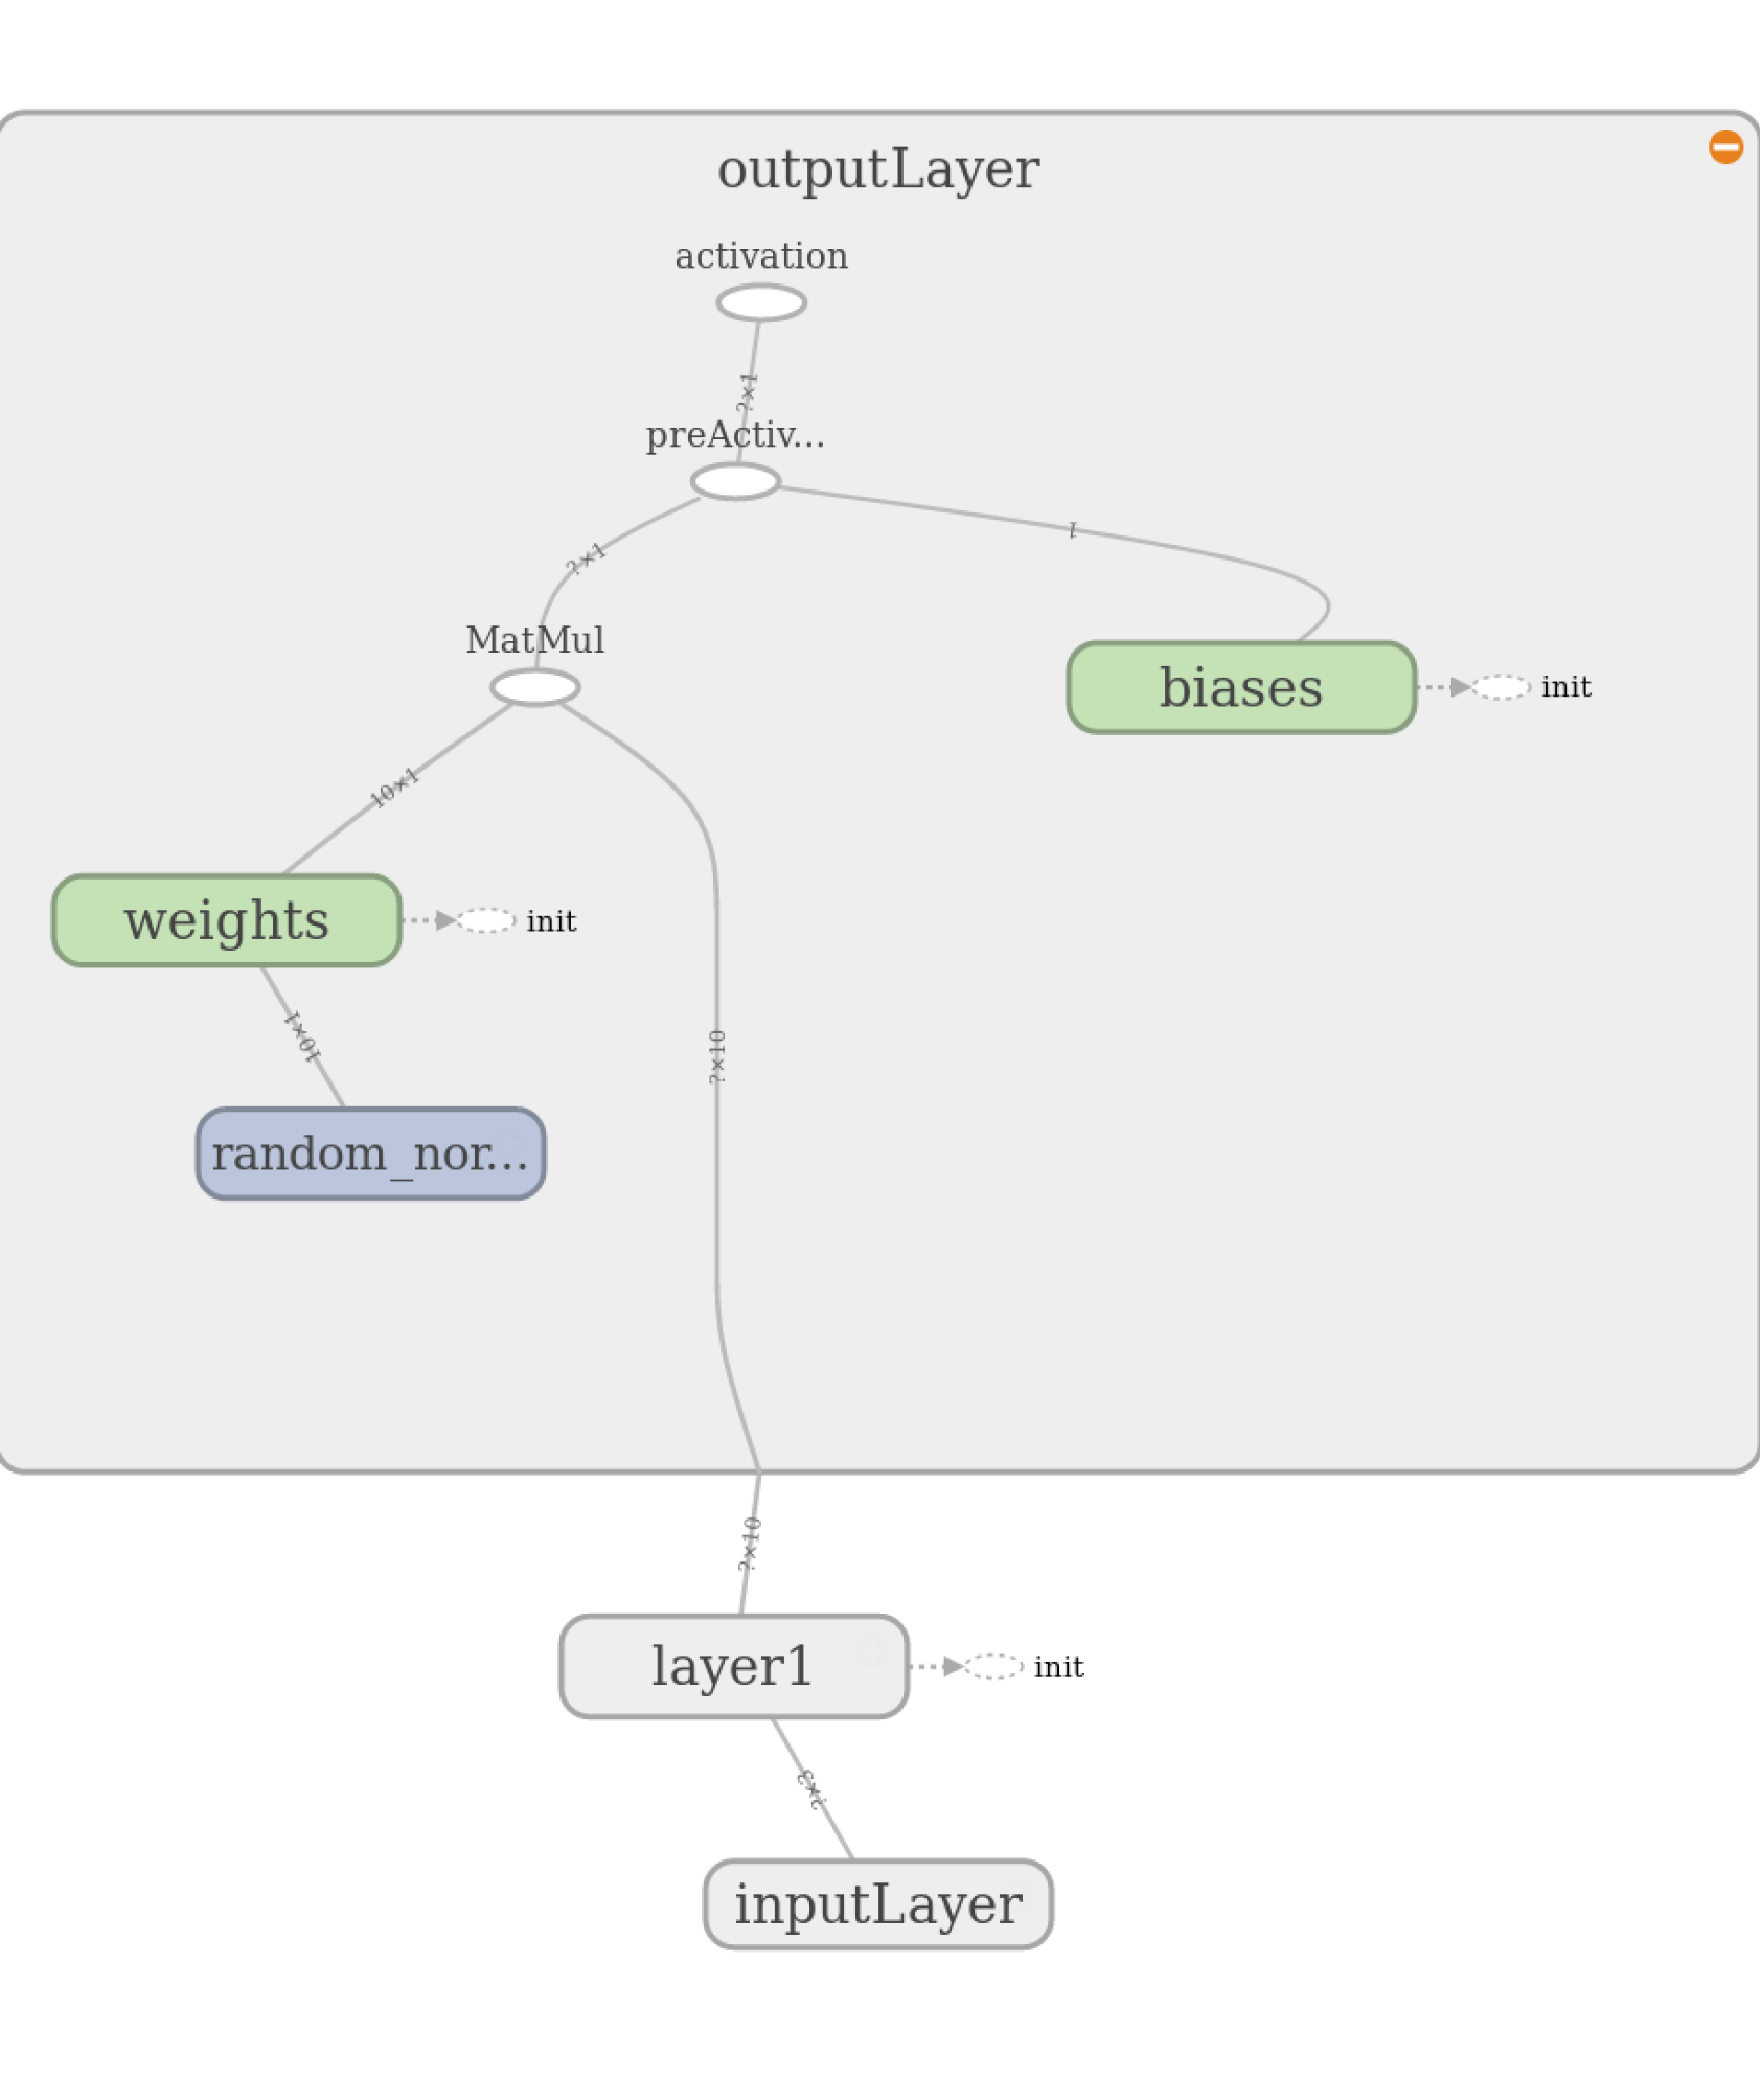
\includegraphics[width=\linewidth]{Figures/Implementation/tensorBoardExample.pdf}
  \caption{Example of a computational graph in TensorBoard of a NN consisting of an input layer, one 
	   hidden layer and an output layer. Nodes are marked by ellipses, the rectangles are namespaces
	   containing several nodes.} 
  \label{fig:graphExample}
\end{figure}
Next, we will demonstrate how to train a NN with TensorFlow. 

\subsection{Training a NN with TensorFlow}
To train the NN described in the previous section, we need two additional components:
a cost function and an optimizer. The cost function expresses the error of the NN fit, while
the optimizer employs an algorithm to minimize this error. The most widely used cost function
for regression with NNs is the L2 norm \eqref{quadraticCostFunction}, which is available as a 
built-in function in TF, \texttt{tf.nn.l2\_loss}. To compute the error, we need to supply known 
target values that is fed into a new \texttt{placeholder},
\begin{lstlisting}[language=Python]
 outputData = tf.placeholder(tf.float32, [None,outputs], name='outputData')
\end{lstlisting}
The cost function is now defined as
\begin{lstlisting}[language=Python]
 trainCost = tf.nn.l2_loss( tf.subtract(actOutput, outputData), name='cost')
\end{lstlisting}
This adds an operation to the graph that calculates the L2 norm of the error between the NN prediction \texttt{actOutput}
on the training data 
and the known target values \texttt{outputData}. In this work, the training data is configurations of atoms, 
while the target values are the atomic energies of these configurations. 

A number of gradient descent-based optimizers are implemented in TensorFlow, including
vanilla gradient descent, Momentum \cite{Qian99}, Adagrad \cite{Duchi11}, Adadelta \cite{Zeiler12} and Adam \cite{Kingma14}.
To add an Adam optimizer operation to the graph, we simply write
\begin{lstlisting}[language=Python]
optimizer = tf.train.AdamOptimizer()
trainStep = optimizer.minimize(trainCost)
\end{lstlisting}
To sum up, we have added the following to the script in the previous section (now with name scoping),
\begin{lstlisting}[language=Python]
outputData = tf.placeholder(tf.float32, [None,outputs], name='outputData')

# cost function
with tf.name_scope('cost'):
    error = tf.subtract(actOutput, outputData, name='deviation')
    trainCost = tf.nn.l2_loss( error, name='L2norm')

# optimizer
with tf.name_scope('optimizer'):
    optimizer = tf.train.AdamOptimizer(learning_rate=0.001, name='Adam')
    trainStep = optimizer.minimize(trainCost, name='trainStep')
\end{lstlisting}
\begin{figure}[H]
\centering
  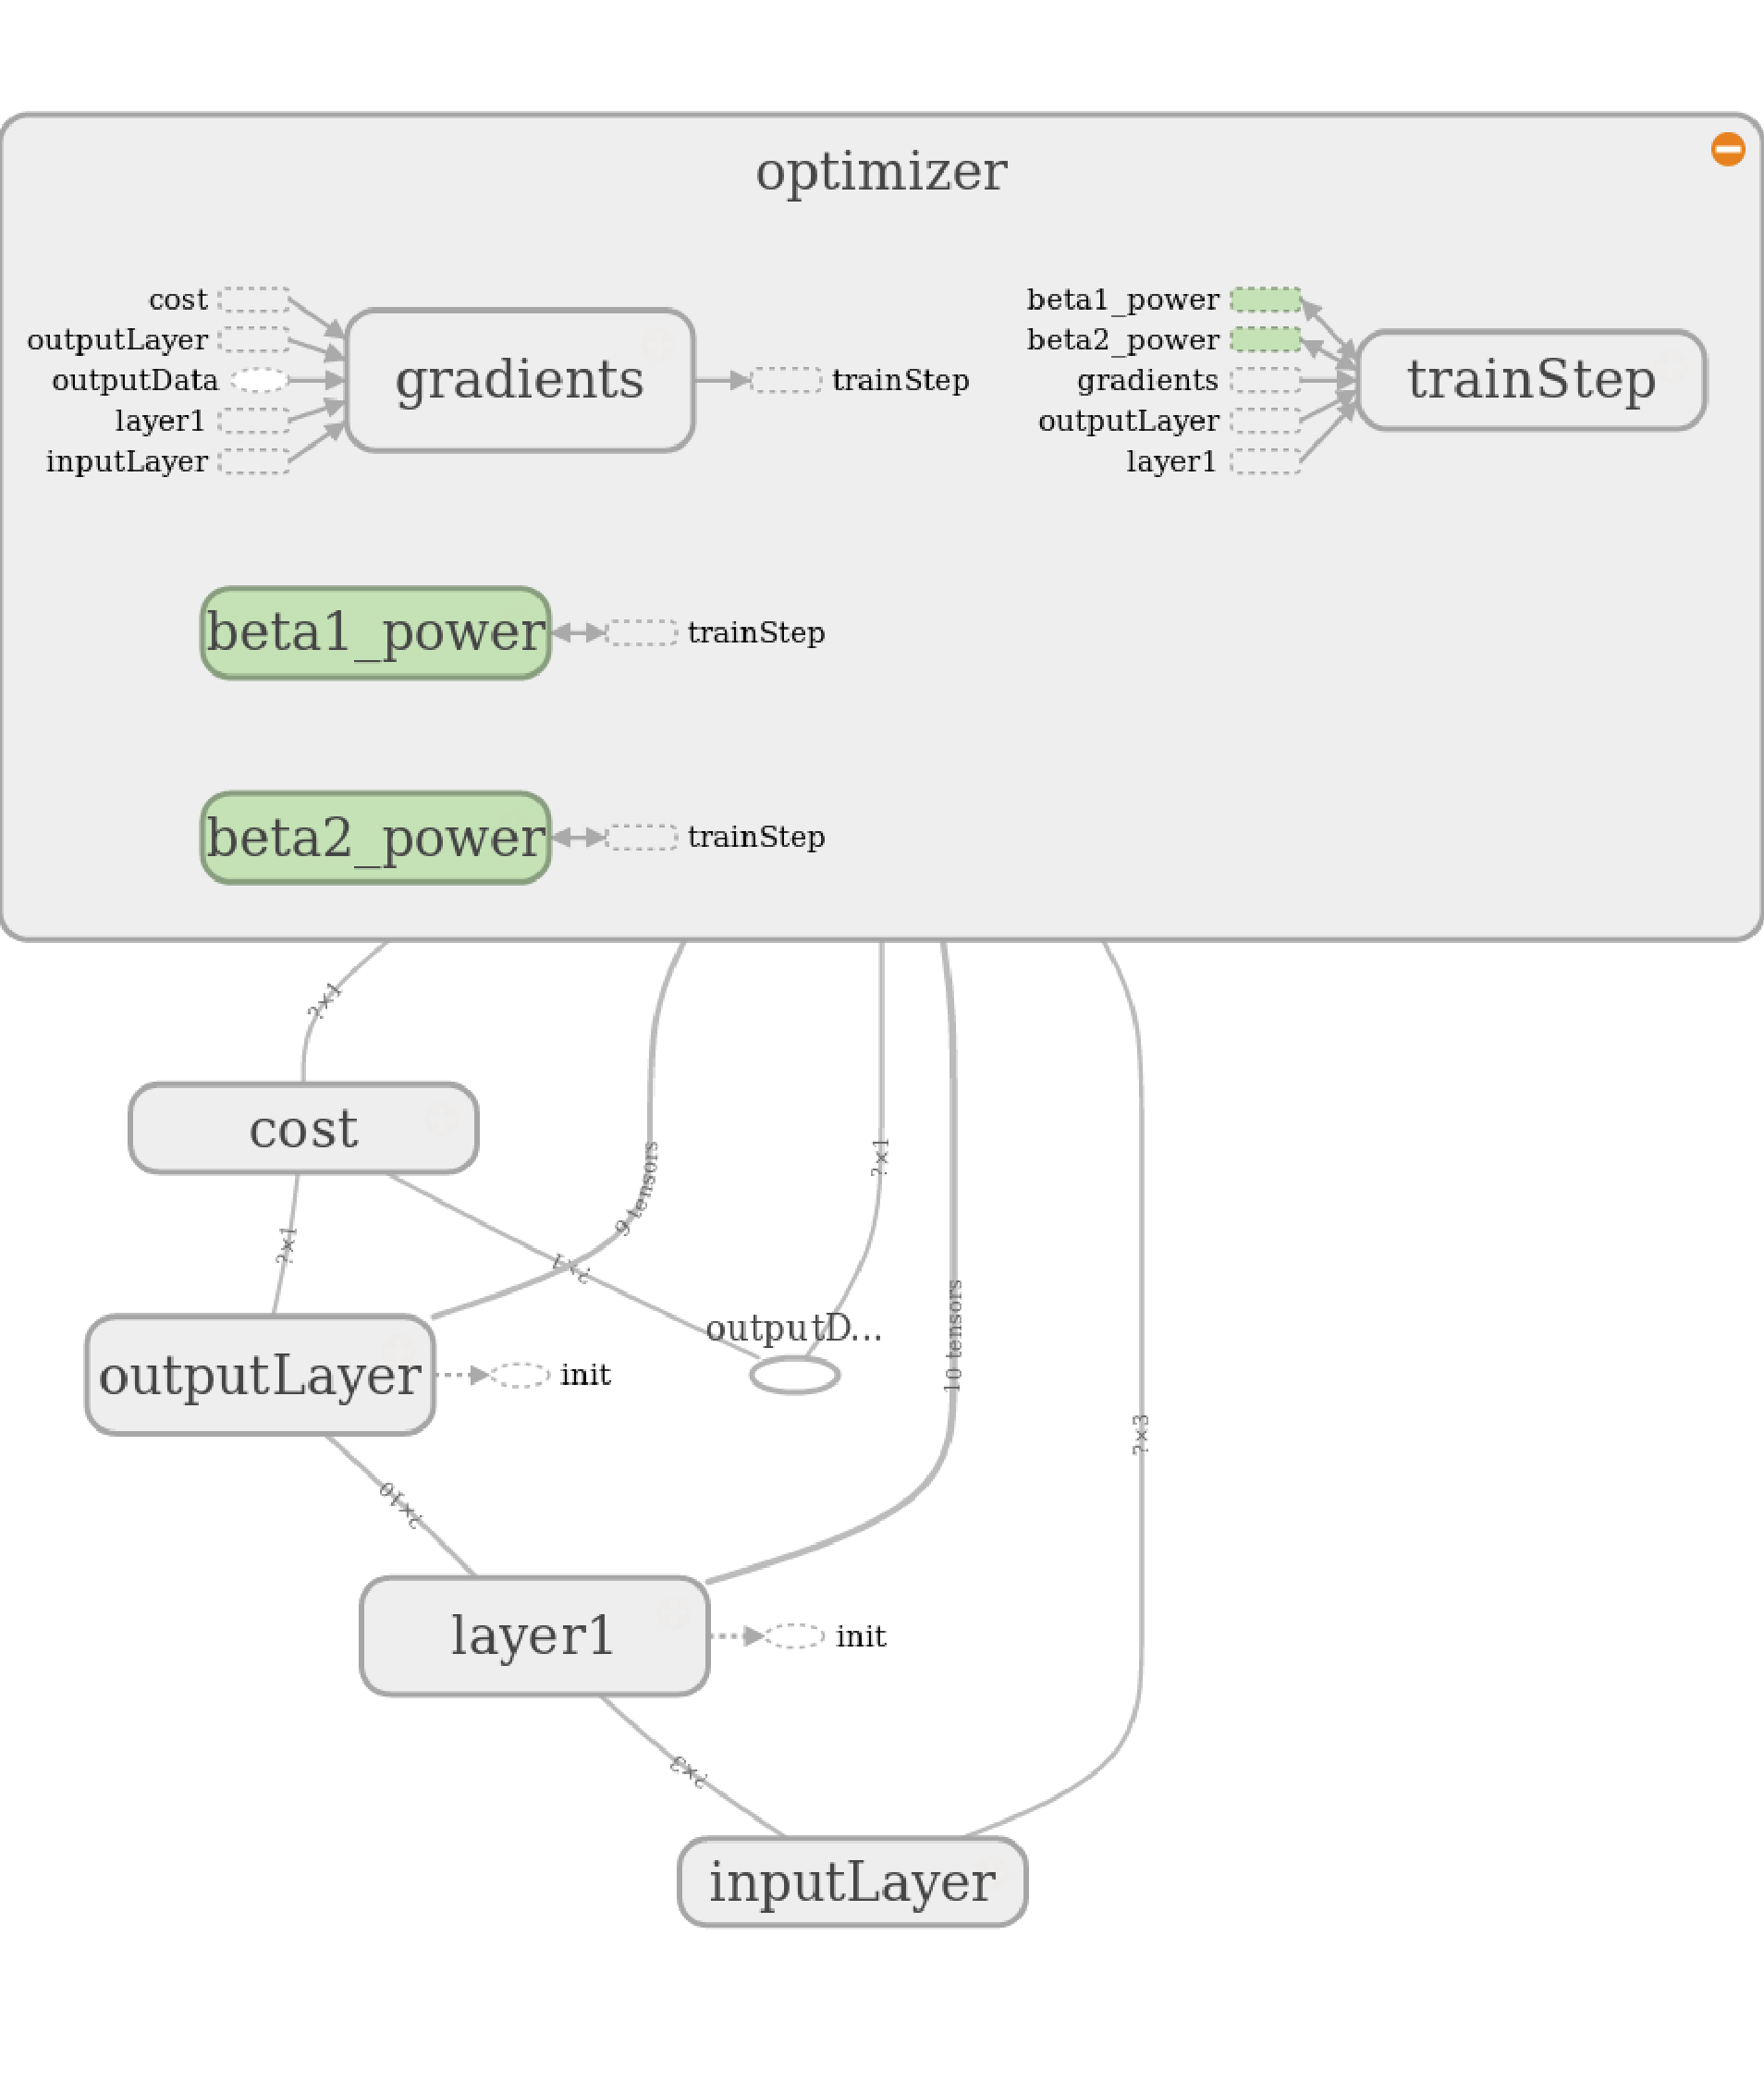
\includegraphics[width=\linewidth]{Figures/Implementation/tensorBoardTraining.pdf}
  \caption{Example of a computational graph in TensorBoard for training a NN consisting of an input layer, one 
	   hidden layer and an output layer. Nodes are marked by ellipses, the rectangles are namespaces
	   containing several nodes. A cost function describing the error of the NN fit and an optimizer that minimizes
	   this error is included in the graph. The optimizer namespace is expanded to display its contents:
	   \texttt{gradients} computes the gradient of all nodes in the graph, \texttt{trainStep} implements
	   the algorithm for updating the NN parameters, while \texttt{beta1\_power} and \texttt{beta2\_power}
	   are the parameters of the Adam optimizer algorithm.}
  \label{fig:tensorBoardTraining}
\end{figure}
The resultant graph can be seen in \autoref{fig:tensorBoardTraining}. 
The optimizer namespace is expanded to display its contents. 
We observe that the optimizer is connected directly to all other parts of the graph, enabling it
to compute the derivative of the cost function with respect to all the weights and biases. This task is
performed by the \texttt{gradients} operation, that in turn sends the total gradient to \texttt{trainStep}, 
which implements the Adam algorithm for updating the NN parameters. 

We are now ready to launch this graph in a training session. 
\begin{lstlisting}[language=Python]
 	
\end{lstlisting}


\chapter{Training procedure}

\section{Selecting the training data}
The number of possible configurations of atomic or molecular systems quickly grows very large. 
Consider for instance water $\textrm{H}_2\textrm{O}$, which is a three-body molecule. The configuration of the
three atoms can be described by three internal coordinates, each with a certain range of values. 
If each range is divided into $N$ equal segments, the total number of distint configurations is $N^3$. 
If we were to construct an \textit{ab inito} potential that characterizes this system, we would have to compute the energies 
and forces of all these configurations. 
Such a brute-force approach may be feasible for a three-atom molecule, but for more complicated systems
it quickly becomes practically impossible due to the computational cost. 

In this work we do not use \textit{ab inito} methods to compute energies and forces, but this problem is still highly relevant
due to the high-dimensional nature of our approach. The average number of neighbours for the Stillinger-Weber Si simulations
in this thesis is about $n=6$, which is a small number compared to most other systems.  
This number is of great importance to the efficiency of the fitting process because it defines the dimensionality 
of the problem,
\begin{enumerate}
 \item When increasing $n$, each symmetry function is composed of 
 more terms. The number of terms $N_{terms}$ scales like $N_{terms} \propto n$ for the radial symmetry functions, 
 but for the angular symmetry functions we have that $N_{terms} \propto n^2$. 
 \item A larger $n$ leads in general to a larger configuration space to fit, thus additional symmetry functions and 
 a larger data set is required. 
 \item The number of NN parameters must also be increased to obtain the same error as for a lower-dimensional problem
\end{enumerate}
These observations demonstrate that performance is a critical factor whether we fit \textit{ab inito} data or 
not. However, we know that only a small subset of the possible configurations of a system is physically realizable. 
Most of the configurations will not be visited by a system obeying Newton's laws, and are therefore not important to
the dynamics. We thus need some kind of importance sampling method that adequately samples this subset. 
We realize that the obvious way to achieve this is to sample configurations from molecular dynamics simulations, which
yields precisely the subset we are looking for. 

\subsection{Iterative molecular dynamics sampling}
The method for constructing a NN PES with data sampled from MD simulations is as follows \cite{Behler11general}
\cite{Behler15},
\begin{enumerate}
 \item Sample an initial data set from MD simulations. \label{sample} 
 \item Calculate the energies and optionally the forces of this initial data set with a chosen method. \label{refEnergies}
 \item Train a NN on the data from \ref{sample}. with reference values from \ref{refEnergies}. to
 construct a preliminary NN potential.
 \item Carry out simulations using the NNP to find new relevant structures. 
 \item Compute the energies (and forces) of the new structures with the method from 2. and add them to the data set
 \item Train a NN on the extended data set to improve the NNP
 \item Repeat 4.-6. until a stopping criteria is met
  \label{NNPalgorithm}
\end{enumerate}
The idea is to improve the NN potential iteratively and in a self-consistent 
way by applying it in MD simulations to find 
''holes'' in the data set, i.e. configurations on which the NNP predicts incorrect energies and forces. The process
is a bit different depending on whether we are constructing a NNP from \textit{ab inito} electronic structure data
or reproducing known, empirical MD potentials. 

For the latter, we construct the initial data set by sampling configurations from MD simulations that is relevant
for the intended applications of the NNP. Furthermore, we are extracting both coordinates and energies from the simulations, i.e.
we get both the training data in step 1 and the reference data in step 2 simultaneously. To compute the energies in
step 4, we simply run a pseudo-simulation on the new structures. This is easily done in LAMMPS by using 
the \texttt{rerun} command, which tells LAMMPS to compute the energies and forces of atomic configurations 
supplied from file without doing any integration. 

When constructing an \textit{ab inito} NNP however, we are immediately faced with a problem when trying to execute this process: 
to run MD simulations in step 1 we need the PES we are trying to develop. 
This is often termed as the ''self-starting problem'', 
and several procedures have been suggested for handling it. 

One option is obviously to generate random configurations. This does however take us back to the 
original problem discussed in the beginning of this chapter: the large configuration space volume of
high-dimensional systems enforces the use of importance sampling methods. 
It is highly unlikely that random sampling will yield the important regions of configuration space, thus 
vast amounts of data is needed. Nonetheless, random sampling can be applicable to small systems of 1-3 atoms where
the complete configuration space can be represented without too much effort. 

Another option is to use chemical intuition to select certain configurations of 
the system under investigation. 
For instance, if a specific chemical reaction is studied, one can use previous knowledge about this reaction to 
select configurations along the reaction path \cite{Ischtwan94}. The disadvantage of this approach is that
such information is not always available. 

A more effective method has been presented by Raff et al. \cite{Raff05}, where a semi-empirical
potential has been deployed to initiate the sampling. If a reasonable potential is chosen and an adequate
sampling method is devised (discussed below), several thousand physically relevant structures can be obtained
that will constitue the initial data set. It has also been shown \cite{Raff05} that the final PES obtained 
by the iterative sampling of MD trajectories is not sensitive to the choice of the empirical surface employed 
in the initial step. 

In this thesis we do not construct \textit{ab inito} NNPs, thus we will not go into further details
of the above methods. 

\subsection{Sampling algorithms}
We have seen that MD simulations supply the data that is needed to construct a NN potential, but we 
also have to consider how this sampling should be performed to identify new relevant structures.
NNs have a very flexible functional form which makes them able to accurately fit data sets, 
but they can also yield potentially large energy and force errors 
when evaluated for configurations that are very different from the ones included in the training set.
It is therefore of vital importance to include all structures that are relevant for the intended
application of the NNP.

Sampling methods should in general be optimized to produce a reasonably uniform density of 
data points in those regions of configuration space that are relevant to the application of the fit \cite{Raff12}. 
If there are regions with very high point density compared to others, the NN will be trained to accurately fit these, 
at the cost of regions that are poorly represented. An exception to this rule is regions where the potential gradient, or forces, 
are large. These regions, typically configurations where two atoms are close to each other and experience strong
repulsive forces, are the most difficult for the NN to fit (REFERENCE?), 
and should therefore have a higher density. 

\subsubsection{Initial sampling}
The initial data set is supposed to function as a starting point for the construction of the NNP. 
In this work we use empirical MD potentials to do the initial sampling. Before the process is initiated, 
we must decide on the specific application for the NNP that we want to develop. This entails 
defining a range of temperatures, pressures etc. that the final NNP will be valid for, and sample
configurations based on these. 

The time interval between selecting configurations during the MD simulations must also be decided. 
One alternative is to simply sample points at constant time intervals. This approach will
however result in a non-uniform density of data points considering that atoms spend most of their time
in regions where the forces are small, at least in equilibrium MD. 

To sample configuration space with something close to a uniform density, the time interval $\tau$ between 
sampling needs to be a function of the atomic accelerations (or forces). One such variable 
interval sampling algorithm, suggested by Pukrittayakamee et al. \cite{Pukrittayakamee09}, is given as
\begin{equation}
 \tau = 
\begin{cases}
\textrm{floor}\left[\alpha/a_{\textrm{max}}\right]\Delta t, 
&\textrm{if floor}\left[\alpha/a_{\textrm{max}}\right] > 0 \\
\textrm{floor}\left[\alpha/a_{\textrm{max}}\right]\Delta t + \Delta t, 
&\textrm{if floor}\left[\alpha/a_{\textrm{max}}\right] = 0
\end{cases}
\label{variableIntervalSampling}
\end{equation}
where $a_i$ is the absolute value of the acceleration of atom $i$, $\Delta t$ is the integration step size, 
$a_\textrm{max}$ is the maximum acceleration of a chosen molecule and $\textrm{floor}(x)$ yields
the integer part of $x$. The constant $\alpha$ is system dependent and must be determined empirically. It is the value 
of $\alpha$ that determines the sampling frequency. We see from the second condition in \eqref{variableIntervalSampling} that
configurations with an acceleration $a_i > \alpha$ yields $\tau = \Delta t$, i.e. the shortest possible sampling
interval. On the other hand, if $a_i < \alpha$, the interval increases by a factor $\textrm{floor}(\alpha/a_\textrm{max})$. 
This approach ensures that we sample all configurations where the gradient of the PES is large, while skipping many
of the low-gradient regions of configuration space. 

We have chosen to use the forces $|\vec{F}_i| \propto a_i$ instead of the accelerations, simply because they are
readily available in LAMMPS. When sampling systems with periodic boundary conditions, we have to consider 
the way forces are updated during a simulation. In LAMMPS, any forces attributed to ghost atoms are added back 
to the originals after \textit{all} forces are computed. This is done in
\texttt{verlet.cpp},
\begin{listing}[H]
 \begin{minted}{c++}
  if (pair_compute_flag) force->pair->compute(eflag,vflag);
  // ...
  if (force->newton) comm->reverse_comm();
 \end{minted}
\end{listing}
The first line computes the forces on all atoms with the chosen \texttt{pair\_style} potential, while
the second line communicates the forces on ghost atoms back to the original atoms according to Newton's third law. 
This means that to employ the algorithm
\eqref{variableIntervalSampling}, we need to sample configurations \textit{after} this reverse communication is
executed, if not the forces will be incorrect. This can be achieved by extending LAMMPS with a new \texttt{compute} 
(described in \autoref{sec:extendingLammps}), as all \texttt{computes} and \texttt{fixes} are invoked after the
force calculations. 

We have made an additional modification to the algorithm \eqref{variableIntervalSampling}.  
Pukrittayakamee et al. \cite{Pukrittayakamee09} sample \texttt{clusters} of atoms for subsequent DFT calculations
of the energies of these clusters, and computes $\tau$ based on the maximum acceleration of an atom in a cluster. 
Our strategy is to select a few atoms, usually 1-10, and compute $\tau$ seperately for each of these atoms. When 
the sampling criterium is met, the coordinates of all neighbours relative to the central atom is written to file, 
as well as the atomic energy the central atom experiences in the presence of its neighbours. These coordinates
and energies make up the training data and reference values, respectively, for a NN to interpolate. 
Our modified sampling algorithm is thus as follows (written in a less convoluted way than above),
\begin{equation}
 \tau = 
\begin{cases}
  \textrm{floor}\left[\alpha/F_i\right], &F_i \leq \alpha \\
  1, &F_i > \alpha \\
  \tau_\textrm{max}, &\textrm{floor}\left[\alpha/F_i\right] > \tau_\textrm{max}
\end{cases}
\label{samplingAlgorithmModified}
\end{equation}
where $\tau$ is measured in units of $\Delta t$ and $\tau_\textrm{max}$ is the maximum value of $\tau$.
$F_i$ is the total force on atom $i$ including ghost contributions. 
We have implemented this sampling algorithm as follows,
\begin{listing}[H]
\begin{minted}{c++}
// ...
// loop through atoms that is to be sampled
for (auto ii : chosenAtoms) {
    i = ilist[ii];
    itype = type[i]-1;

    double F = sqrt(f[i][0]*f[i][0] + f[i][1]*f[i][1] + f[i][2]*f[i][2]);

    // update tau every maxDelay step
    if ( !(myStep % maxDelay) ) {

      // no delay if force is larger than alpha
      if (F > alpha[itype]) tau[atomCount] = 1;

      // calculate delay if force less than alpha
      else {
        int factor = floor( alpha[itype] / F );
        if (factor > maxDelay) tau[atomCount] = maxDelay;
        else                   tau[atomCount] = factor;
      }
    }

    // decide whether to sample or not based on current value of tau for atom i
    if ( (myStep % tau[atomCount] > 0) && useAlgo) continue;

    double xi = x[i][0];
    double yi = x[i][1];
    double zi = x[i][2];
    
    // loop through neighbours of atom i 
    // write relative coordinates and atomic energy to file
    jlist = firstneigh[i];
    jnum = numneigh[i];
    for (jj = 0; jj < jnum; jj++) {
      j = jlist[jj];
      // ...
\end{minted}
\end{listing}
The vector \texttt{chosenAtoms} contains the indicies of the atoms that are to be sampled. These indicies are decided
when the parameters of the employed potential is initiliazed with the input script command \texttt{pair\_coeff}. 
The variable \texttt{maxDelay} decides how often $\tau$ is updated, and functions as a maximum value of $\tau$. 
Its value does not change in the course of the simulation. 
\begin{figure}[H]
\begin{minipage}[t]{0.48\linewidth}
  \subcaption{}
  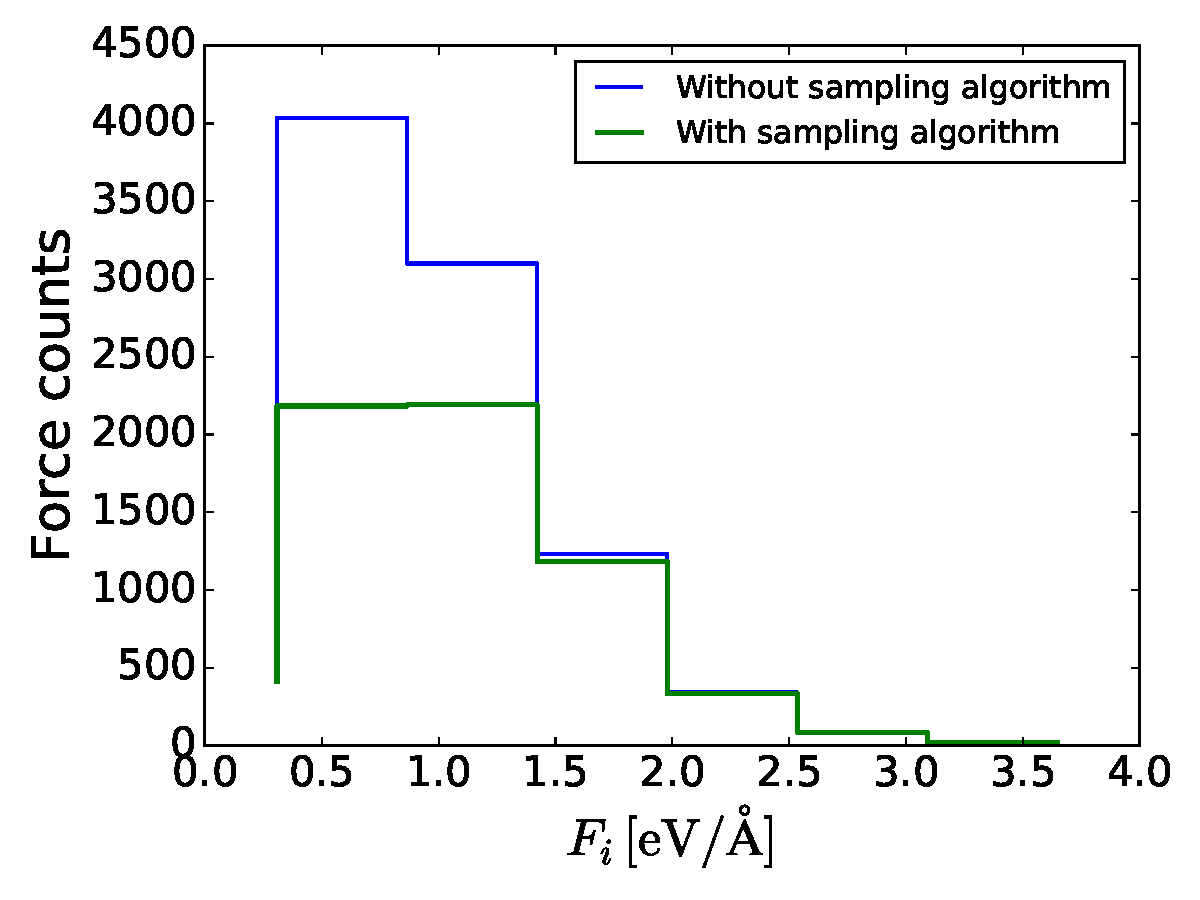
\includegraphics[width=\textwidth]{Figures/Implementation/forceDistSamplingAlgo.pdf}
\end{minipage}
\quad
\begin{minipage}[t]{0.48\linewidth}
\subcaption{}
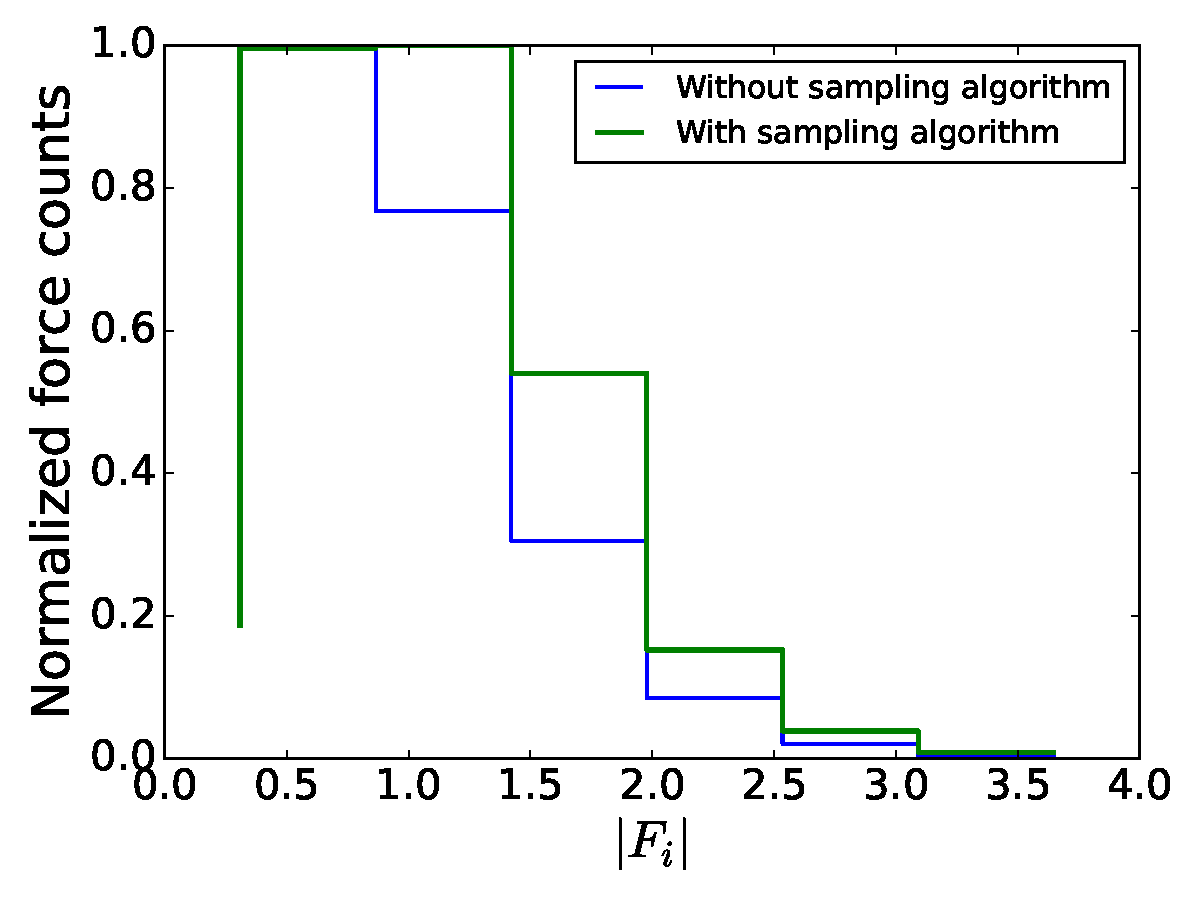
\includegraphics[width=\textwidth]{Figures/Implementation/forceDistSamplingAlgoNormed.pdf}
\end{minipage}
  \caption{Distribution of forces for one Si atom in a quartz $\textrm{SiO}_2$ crystal with 
	   and withouth the use of the sampling algorithm \eqref{samplingAlgorithmModified}. 
	   The crystal consists of 576 atoms, with an initial temperature $T= \SI{1000}{\kelvin}$, 
	   run for $N = 10000$ time steps. The atoms are sampled from the microcanonical ensemble with
	   periodic boundary conditions.
	   Sampling algorithm parameters: $\alpha=3.0$ and 
	   $\tau_\textrm{max} = 10$.}
\label{fig:forceDistSamplingAlgo}
\end{figure}
\autoref{fig:forceDistSamplingAlgo} displays the distribution of forces for one Si atom in a MD simulation
of quartz $\textrm{SiO}_2$, with and withouth the use of the sampling algorithm \eqref{samplingAlgorithmModified}. 
We see from the figure a) that the sampling procedure cuts the number of low-gradient configurations significantly, 
while keeping all the environments corresponding to large forces. The resulting distribution is however not uniform, simply
because the ratio of force counts in the range $F_i = \SIrange{0}{2}{\angstrom}$ to the range $F_i = \SIrange{2}{4}{\angstrom}$
is too high originally.

One way to smooth the distribution further is to manually delete configurations after the simulation 
is finished, but then we risk removing relevant structures. The gradient of the PES is not the only way 
to measure the quality of the sampled set, the time aspect is also important. 
By selecting samples on-the-fly, we are guaranteed that the they are distributed somewhat uniformly in the time domain. 
Deleting structures blindly subsequent to the simulation is therefore not a good idea (I AM NOT SURE IF THIS IS TRUE, 
HAVE TO BE TESTED).

Another option is to sample different types of systems where the forces are more evenly distributed. 
Examples are non-periodic systems or systems containing only a few atoms. Also, it can be a good idea 
to do short simulations where the atoms start out in non-equilibrium positions to obtain configurations
that are not visited by systems with a regular lattice initial state. 
In general, it is not required that the data used to train the NNs are the results of physically plausible 
simulations, the only requirement is that it should cover all possible configurations that the NNP have the possibility
of experiencing in the course of its application. WRITE MORE / DO TESTS ON THIS???

\subsubsection{Iterative sampling}
The initial data set is usually not sufficient to construct a stable neural network PES. 
It is difficult to identify all the relevant structures that the NN have to learn to perform well, and 
since there is always a small fitting error, the 
NNP will generate different trajectories than the PES that has been used to train it. This is solved
by sampling new relevant structures from simulations using the preliminary NNP trained on the initial data set. 
In this way, new configurations
will ''naturally present themselves'', and the NNP will iteratively improve in a self-consistent way.

The obvious way to identify new structures not already in the initial data set is to evalate both the NNP and 
the PES we are trying to fit for each structure in an NNP MD simulation and compare the energies (and eventually 
the forces). If the energy deviation is above a certain treshold, the structure is added to the training set.
This can be done for different temperatures, pressures etc., and after a certain amount of new data is added, 
the NN is trained on this extended data set and thus improved. Then, new simulations are carried out with the improved
NNP, according to the iterative process \autoref{NNPalgorithm} described in the beginning of this chapter. 

This approach is easily feasible when the target PES is an empirical potential, but too computationally expensive 
in the case where electronic structure methods are employed. Raff et al. \cite{Raff05} have developed a sampling
algorithm called \textit{modified novelty sampling} that does not require any quantum mechanical calculations of
the energies of new structures. They describe the database as a set of vectors $\{\vec{q}\}$, where vector
$\vec{q}_i$ contains the internal coordinates of the $i_\textrm{th}$ cluster of atoms. New configurations
$\vec{q}_n$ are generated using the NNP trained on this data base and the 2-norm difference $\vec{d}$ between vectors
$\vec{q}_n$ and $\vec{q}_i$ are computed,
\begin{equation}
 \vec{d} = | \vec{q}_i - \vec{q}_n | = 
 \left[(\vec{q}_i - \vec{q}_n)\cdot(\vec{q}_i - \vec{q}_n)\right]^{1/2}
\end{equation}
for all clusters $i$. The difference vector is characterized by its minimum value $d_\textrm{min} = \textrm{min}(\vec{d})$ and 
the mean seperation distance $d_\textrm{mean} = \langle\vec{d}\rangle$. 
The basic idea is to add configuration point $\vec{q}_n$ to the database with high
probability if $d_\textrm{min}$ or $d_\textrm{mean}$ is large, but low probability if both 
$d_\textrm{min}$ and $d_\textrm{mean}$ are small. The energy output of the NNP are also included in the scheme, along with
a more involved selection algorithm. As this thesis only deals with empirical target potentials, the details will
not be further discussed here. 

In this work we use the Behler symmetry functions to transform atomic cartesian coordinates to vectors of symmetry values.
These functions act as descriptors of chemical environments, and should therefore be excellent candidates
to identify relevant structures during MD simulations without computing additional target energies. 
Behler has suggested two methods \cite{Behler15} where these symmetry functions are employed to improve the NNP. 
The first and simplest method identifies structures that fall outside of the range of input values spanned by the training data. 
This is achieved by comparing the symmetry function vector of each atom during the MD simulation with 
the minimum and maximum values of each symmetry function in the database for the respective element. 
When such configurations are encountered, a warning can be issued and the structure sampled. 
These kind of configurations are important to identify, as NNs have very limited extrapolation abilities. 

The other kind of ''unknown'' structures are those within the range of existing symmetry values, but located
in parts of configuration space that is poorly represented in the training set. 

REMEMBER TO ADD UNITS TO ABOVE FIGURE


SAMPLING FILOSOFI sum up:
USING THE ABOVE ALGORITHM TO MAKE SURE I SAMPLE ALL THE CONFIGS THAT CORRESPOND TO LARGE FORCES ON CENTRAL ATOM.
THIS IS ENSURED BY SETTING ALPHA TO ABOUT 2.0 FOR SIO2 AND RESTRICT THE VALUE OF TAU TO ABOUT 20-30. 
AFTERWARDS, I DELETE A LOT OF THE LESSER FORCES. I SHOULD CHECK THAT THIS GIVES A RESONABLE FIRST APPROXIMATION
TO THE NN PES. I SHOULD TRY TO MAKE ONE NET WITH GENERIC SAMPLING, ONE WITH ONLY SAMPLING ALGO, AND ONE WITH BOTH SAMPLING
ALGO AND CUTTING. THE DATA SETS SHOULD BE OF ABOUT EQUAL SIZE. 




There are two types of such ''unknown'' structures. 
First, we have configurations that are outside the range of input values spanned by the training data. 


We already have a tool
for identifying such ''unknown'' structures, namely the Behler symmetry functions. 



\section{Constructing the symmetry function sets}
The choice of symmetry functions is important to achieve a good fit to the reference data. 
They need to be able to sufficiently distinct inequivalent structures to avoid fitting 
contradictory data. If this distinction is not possible, different reference structures with 
different energies and forces give rise to the same symmetry function values, which results in poor fits. 

Although a NN potential is general and unbiased because it has no pre-defined functional form, the 
construction of the symmetry function sets is to some extent empirical. The functional form of the NN
is adjusted ''automatically'' when trained, while the symmetry function set has to be constructed manually.
This observation does however not change the fact that the high-dimensional neural network approach to
constructing potentials used in this work is general, and can in principle be applied to any system. The training data
and symmetry function sets have to be customized to each system, but the training procedure is always the same. 

There are a number of analyses that can be carried out to investigate if we have an adequate
symmetry function set,
\begin{itemize}
 \item The symmetry functions should cover the configuration space evenly. 
 A reasonable initial choice for the radial symmetry functions is to use an equidistant set to ensure 
 that the whole range of distances in the reference set are probed. Also, it is a good idea 
 to have some knowledge about the radial and angular distribution of atoms for the system we are looking at. 
 This information can be extracted from MD runs with semi-empirical potentials or from experiments and will enable
 us to identify high-density regions of configuration space that should be covered by a larger number
 of symmetry functions than low-density regions. HMMMM, THIS IS VERY BIASED?????????? BEHLER SAYS ''IN AND UNBIASED WAY''.
 \item The range of values for each symmetry function should be analyzed. If the difference between the largest
 and smallest function value is too small, it will not be able to identify distinct structures properly. 
 Symmetry functions which have a value of zero for all configurations should be avoided, as these will not contribute
 to the description of the chemical environment. 
 \item SEARCH FOR CONTRADICTORY DATA? THEN I MUST HAVE ACCESS TO THE FORCES? BUT IS HE TALKING ABOUT DIFFERENT 
 ATOM TYPES? MAYBE CHOOSE A NEIGHBOUR LIST (ATOM), FIND $\Delta G$ AND $\Delta F$ TO ALL OTHER LISTS AND PLOT?
 \item There is a trade-off between the ability of the symmetry function set to cover the configuration space and 
 the efficiency of the calculation of the NN energy output. The number of symmetry functions can be kept as low as
 possible by investigating the correlations between the values of two different symmetry functions for the whole
 reference set. If there is a large correlation, the two symmetry functions are almost linearly dependent, 
 and we have a redundancy of information. Consequentially, one of them should be removed, or the parameters adjusted
 to decrease the correlation. WRITE ABOUT CORRELATIONS AND TRAINING. 
\end{itemize}
These tests provide a framework for constructing suitable symmetry function sets. 
We note that they all depend on the composition of the available data set, including its size. 
When the iterative approach to constructing data sets are used, the size will increase step by step, 
and we are required to add more symmetry functions as we go. 



\chapter{Validation}

\section{Time usage} \label{sec:timeUsage}
The workflow when training a NN and using it in MD is as follows: 
\begin{enumerate}
 \item Generate training data
 \item Train a NN to fit the data
 \item Use the analytical expression for the trained NN as a potential in MD
\end{enumerate}
The main application programming interface (API) for TensorFlow (TF) is Python. The NN is therefore
trained using Python scripts, while C++ is utilized to run the MD simulations for speed purposes. Thus
we need a way to transfer the NN from Python to C++. 

There are built-in functions in TF that automatically saves computational graphs (architecture of network plus
nodes for training) and variables (weights and activation functions) as binary files.
These files can then be read and the NN evaluated using the TF C++ API. This API is however quite under-developed
and the documentation is very sparse. Another alternative is to manually save the weights and biases
as a text file, along with information on which activation function(s) that has been used. This file 
file can then be used to reconstruct the NN in the same way that it is made in Python: By representing
the connection weights between layers as matrices and the biases as vectors. The activation functions
must be coded manually. A linear algebra library should
be utilized for speed and simplicity; we have chosen to use Armadillo. 

To find out which alternative is the most efficient for evaluating a NN, we compare the 
time usage in three cases: with TF in Python, with TF in C++ and with Armadillo. 
The results are shown in \autoref{fig:timeComparisonEvaluateNetworkTotalScatter}.
\begin{figure}[H]
\centering
  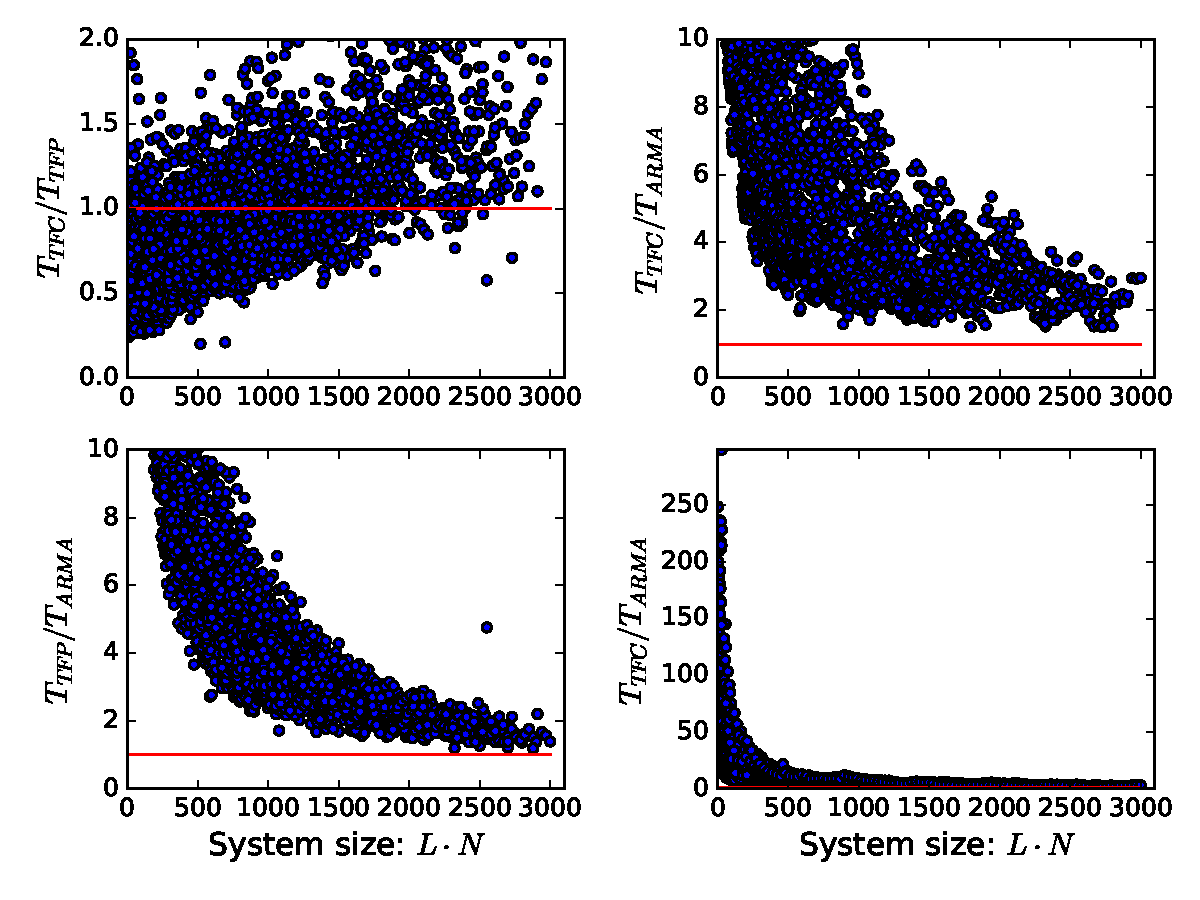
\includegraphics[width = 0.9\linewidth]{Figures/Tests/timeComparisonNetworkTotalScatter.pdf}
  \caption{Scatter plot of CPU time when evaluating untrained NNs with random weights and sigmoid activation functions
	   using the TF Python API ($T_{TFP}$), the TF C++ API ($T_{TFC}$) and Armadillo ($T_{ARMA}$). 
	   $L$ is the number of layers, $N$ is the number of nodes in each hidden layer. All the NNs
	   have one input and one output. The time has been found by averaging over 50 evaluations
	   for each NN architecture. $T_{TFC}/T_{ARMA}$ is also shown in an uncut version to demonstrate
	   how large the time difference is for very small NNs.}
\label{fig:timeComparisonEvaluateNetworkTotalScatter}
\end{figure}
\begin{figure}[H]
\centering
  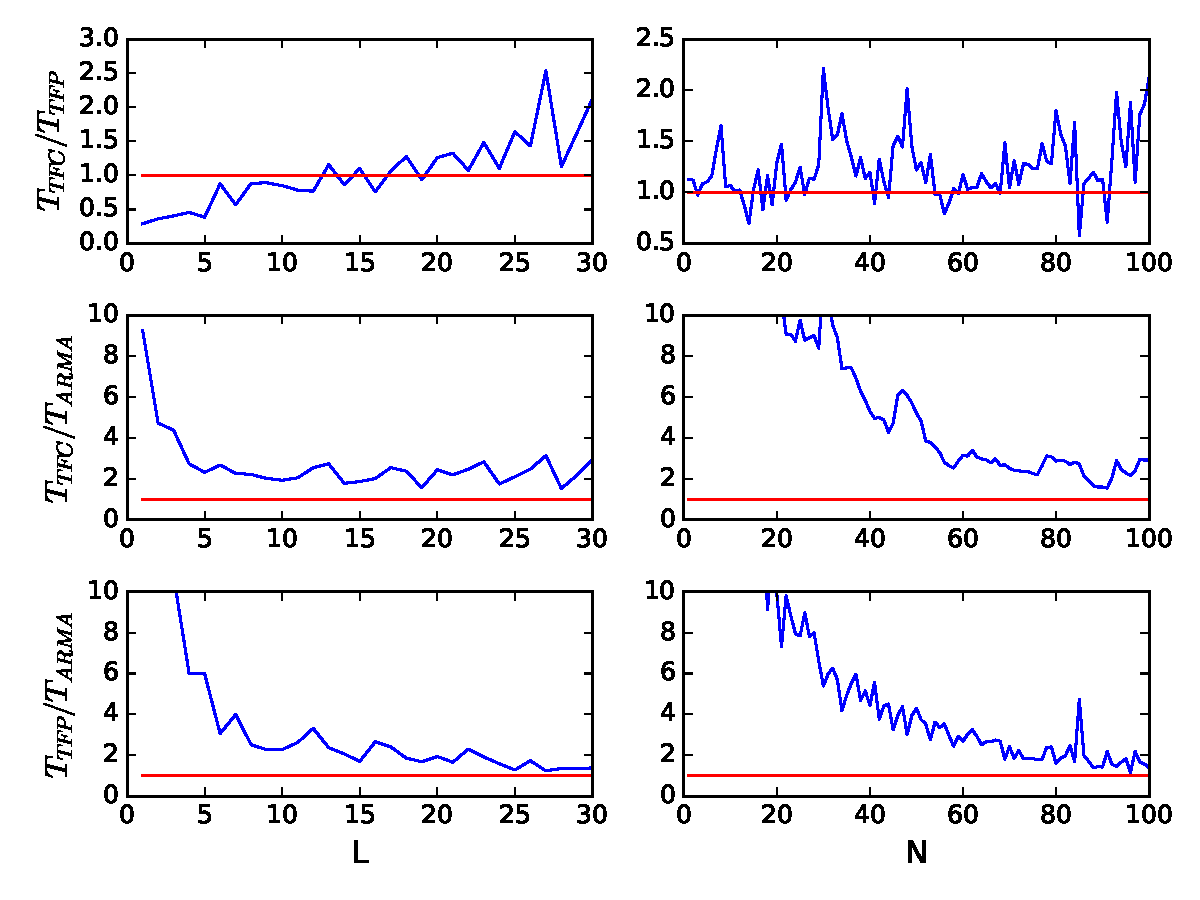
\includegraphics[width = 0.9\linewidth]{Figures/Tests/timeComparisonNetwork3.pdf}
  \caption{Left column: CPU time comparison for $N=100$. Right column: CPU time comparison for $L=30$.} 
  \label{fig:timeComparisonEvaluateNetwork2}
\end{figure}
As we can see, evaluation of an NN with the built-in TF methods are notably slower than with Armadillo 
for small NNs, but seems to converge to 1 for large networks. The convergence rate is however surpisingly low. One reason for this
can be that the \textit{Session} environment in TF has lot of overhead. However, the main computational strength of TF resides 
in GPUs, which will be tested out later on. 


\section{Training Lennard-Jones potential}
To verify that the implementation of the NN and the backpropagation algorithm with Armadillo in our MD code is correct, 
we train a NN to reproduce the shifted Lennard Jones potential (REF TIL LIKNING). 
The error of the trained network on the training data interval is evaluated both in Python and C++. The two error
plots are shown in \autoref{fig:errorLJTest}. 
\begin{figure}[H]
\begin{minipage}[t]{0.48\linewidth}
  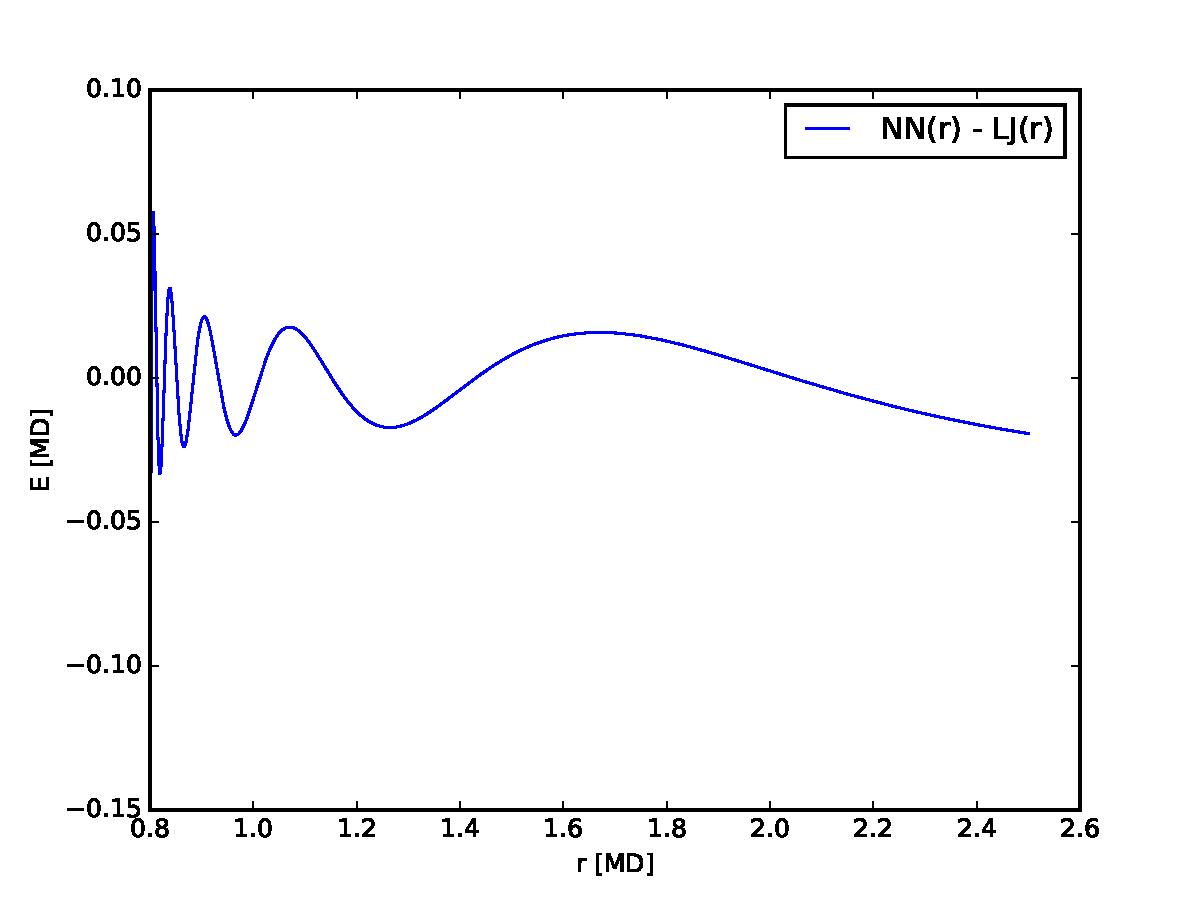
\includegraphics[width=\textwidth]{Figures/Tests/errorLJ.pdf}
\end{minipage}
\quad
\begin{minipage}[t]{0.48\linewidth}
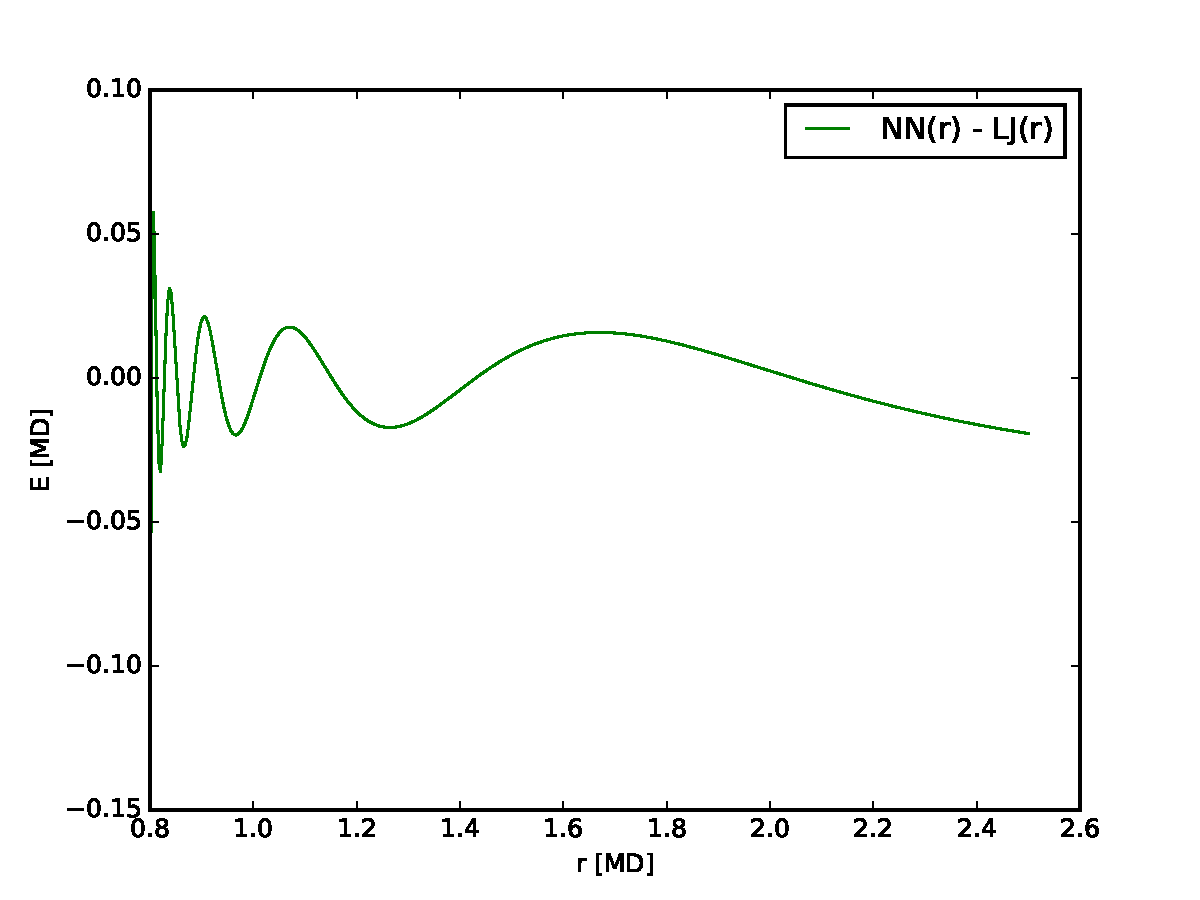
\includegraphics[width=\textwidth]{Figures/Tests/errorLJC.pdf}
\end{minipage}
  \caption{Error of a network trained to reproduce the shifted Lennard-Jones potential. 
           The NN is trained in Python and the error on the training data interval
           is calculated, shown on the left. The NN is also written to file for evaluation in C++, 
           shown on the right.}
\label{fig:errorLJTest}
\end{figure}
We observe that the error has excactly the same shape and value on the whole interval, we can therefore
confirm that the NN is implemented correctly. 

To test the implementation of the backpropagation algorithm, the
same NN is differentiated in C++ and compared to the analytical derivative of the L-J potential. 
The gradient of a NN is defined as the derivative of one of the outputs with respect to the input(s). 
There are two differences when using backpropagation to find the gradient of a network compared
to the use of backpropagation in training:
\begin{enumerate}
 \item The derivative of the output neuron's activation function is backpropagated instead of the output error
 \item We backpropagate all the way down to the input layer, during training we stop at the first hidden layer
\end{enumerate}
As mentioned before, the backpropagation algorithm is simply an application of the chain rule: 
To obtain the derivative of the output node with respect to the input nodes we need to differentiate through
all the nodes in-between because we have fully connected layers. The gradient error is plotted in 
\autoref{fig:errorBackPropTest}.
\begin{figure}[H]
\centering
  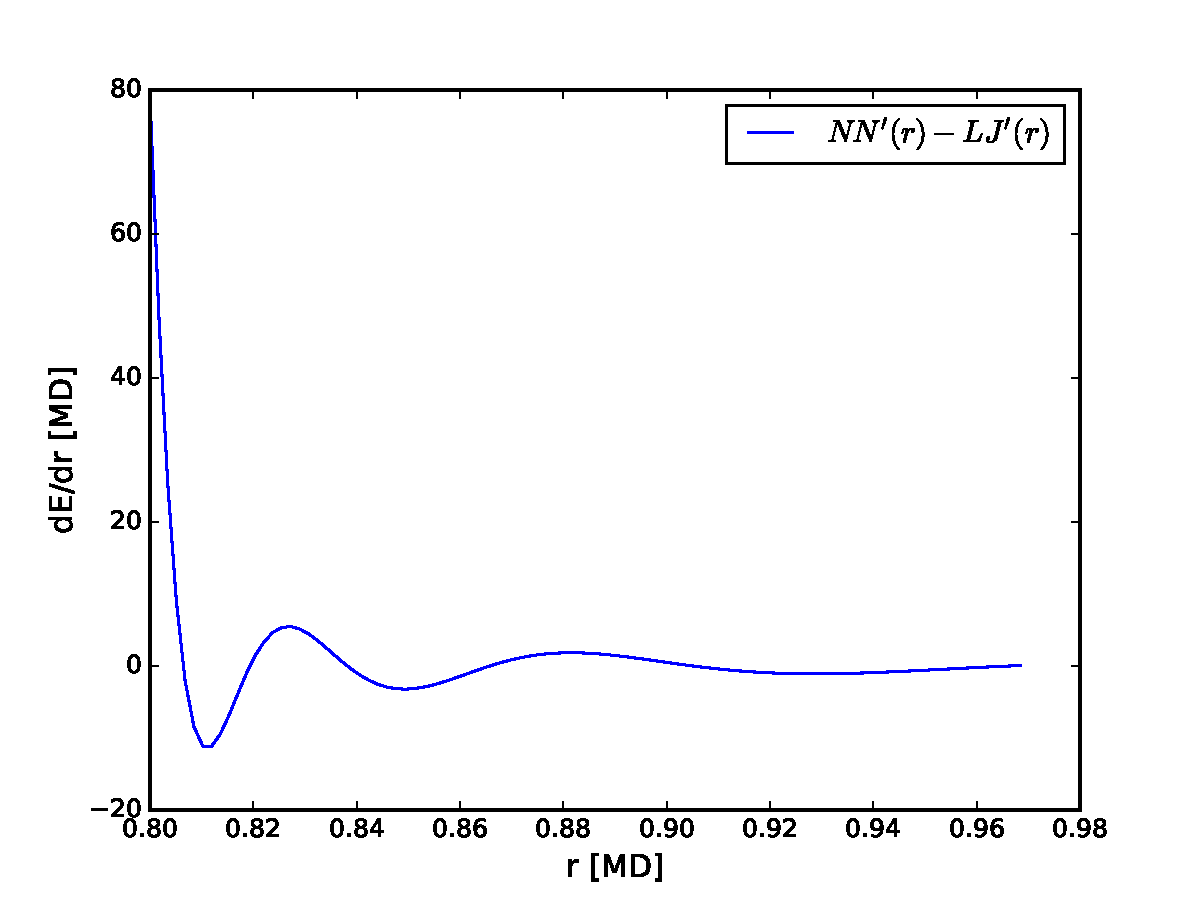
\includegraphics[width = 0.9\linewidth]{Figures/Tests/errorDerivative.pdf}
  \caption{Error of the gradient of a NN trained to reproduce the shifted Lennard-Jones potential.
	   The NN is trained in Python and evaluated and differentiated in C++ using the backpropagation algorithm.
	   The result is compared to the analytical derivative of the LJ potential. Only a part of the training
	   interval is shown, the graph is essentially flat after this point} 
  \label{fig:errorBackPropTest}
\end{figure}
Again we get an oscillating error over the training interval. The oscillations near the left end of the interval is much larger
than for the energy, but they get damped more quickly. The large error near the left end of the interval is a natural
consequence of the shape of the LJ potential for these values: the $1/r^{13}$ term dominates with its very steep slope, the NN is not 
fed a sufficient amount of data in this region to excactly reproduce the rapid changing derivative. 
This tells us that it is important to train the NN on a larger data interval than needed in simulations or possibly
feed the NN more data in critical regions during training. 

\subsection{Many-neighbour Lennard-Jones}
A NN can also be trained to obtain the energy of several neighbouring atoms at once. 
The training procedure is excactly the same, but now we train the network so that the output
is the sum of $N$ LJ-potentials for $N$ different distances $r$. The NN will have $N$ inputs and 1 output. 
To get an error of the same order as for 1 neighbour, we need to have a lot more nodes. The result of a training
session with $N=20$ inputs is shown in figures \autoref{fig:trainingManyNeighbourNN}. 
(Training session 02.12-19.36.50)
\begin{comment}
\begin{figure}[H]
\centering
  \begin{subfigure}[b]{0.75\textwidth}
  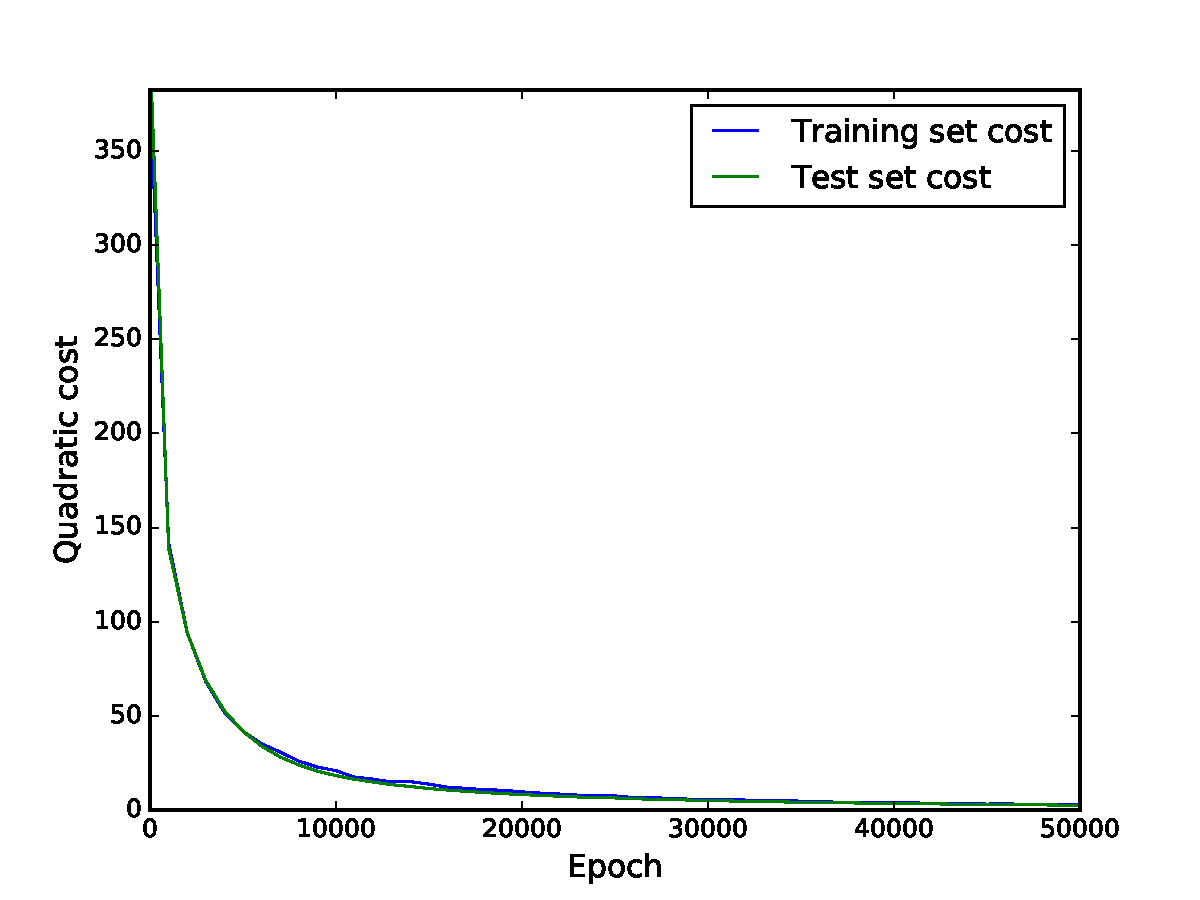
\includegraphics[width = 0.9\linewidth]{Figures/Tests/trainingManyNeighbourNN1.pdf}
\end{subfigure}
\begin{subfigure}
  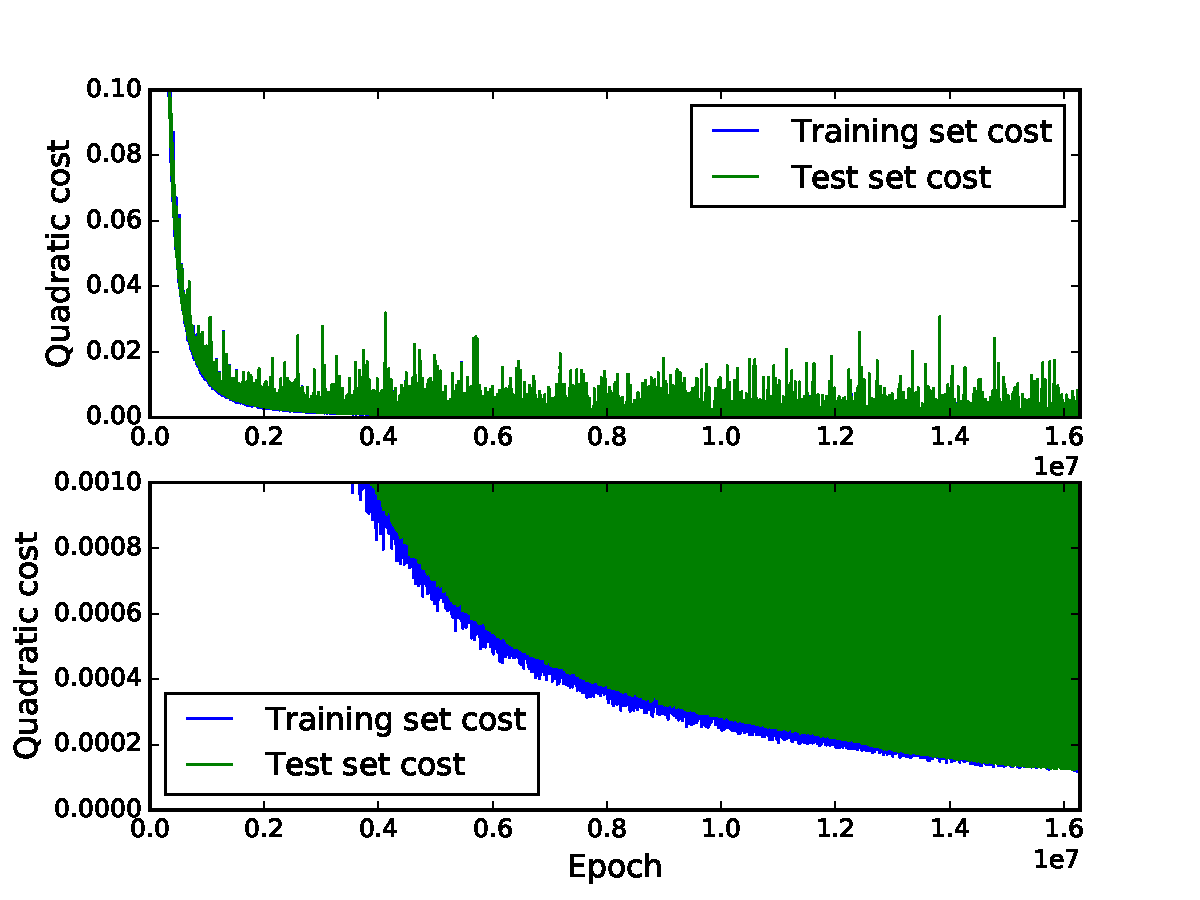
\includegraphics[width = 0.9\linewidth]{Figures/Tests/trainingManyNeighbourNN2.pdf}
  \end{subfigure}
  \label{fig:trainingManyNeighbourNN1}
  \caption{Error of the gradient of a NN trained to reproduce the shifted Lennard-Jones potential.
	   The NN is trained in Python and evaluated and differentiated in C++ using the backpropagation algorithm.
	   The result is compared to the analytical derivative of the LJ potential. Only a part of the training
	   interval is shown, the graph is essentially flat after this point} 
\end{figure}
\end{comment}
\begin{figure}[H]
\centering
\subcaptionbox{Zoomed out\label{zoomedOut}}{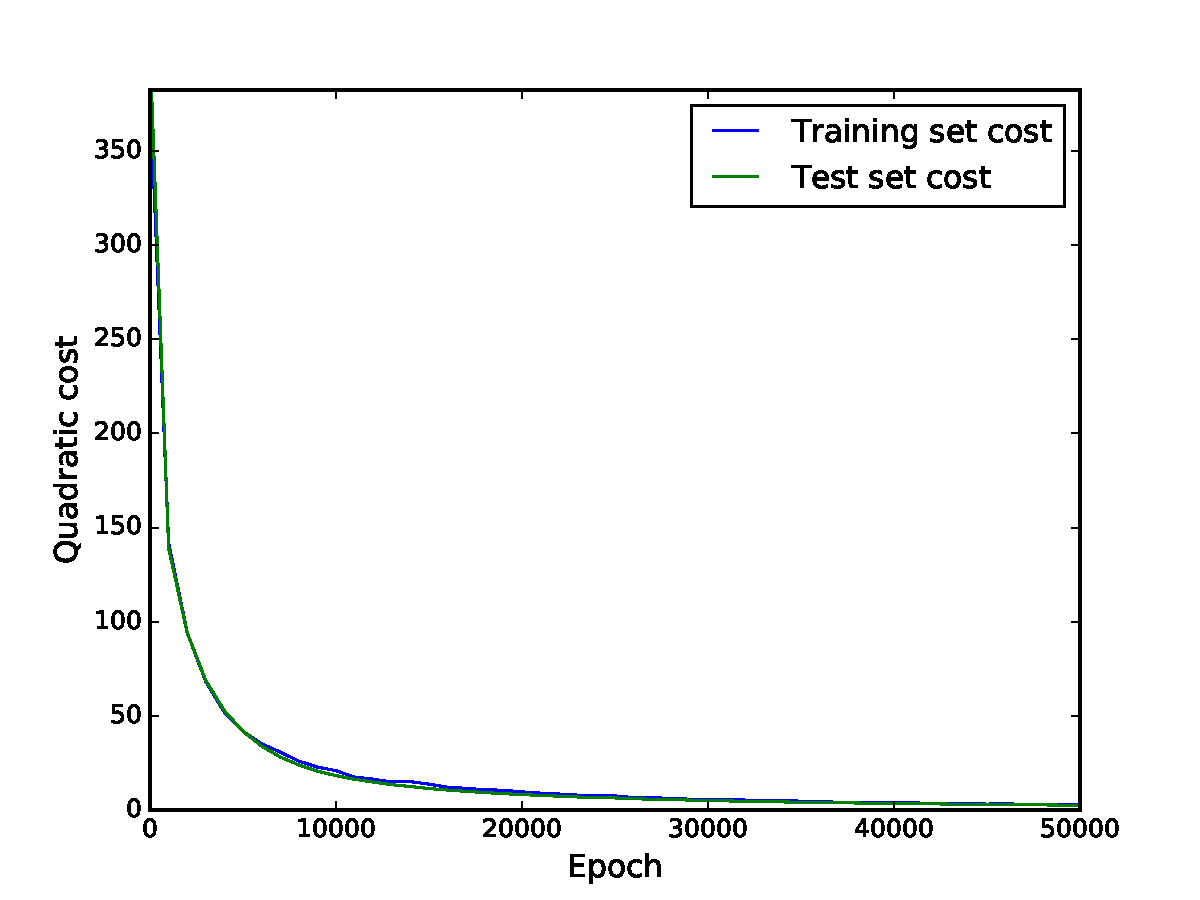
\includegraphics[width=0.8\textwidth]{Figures/Tests/trainingManyNeighbourNN1.pdf}
  }
\subcaptionbox{Zoomed in\label{zoomedIn}}{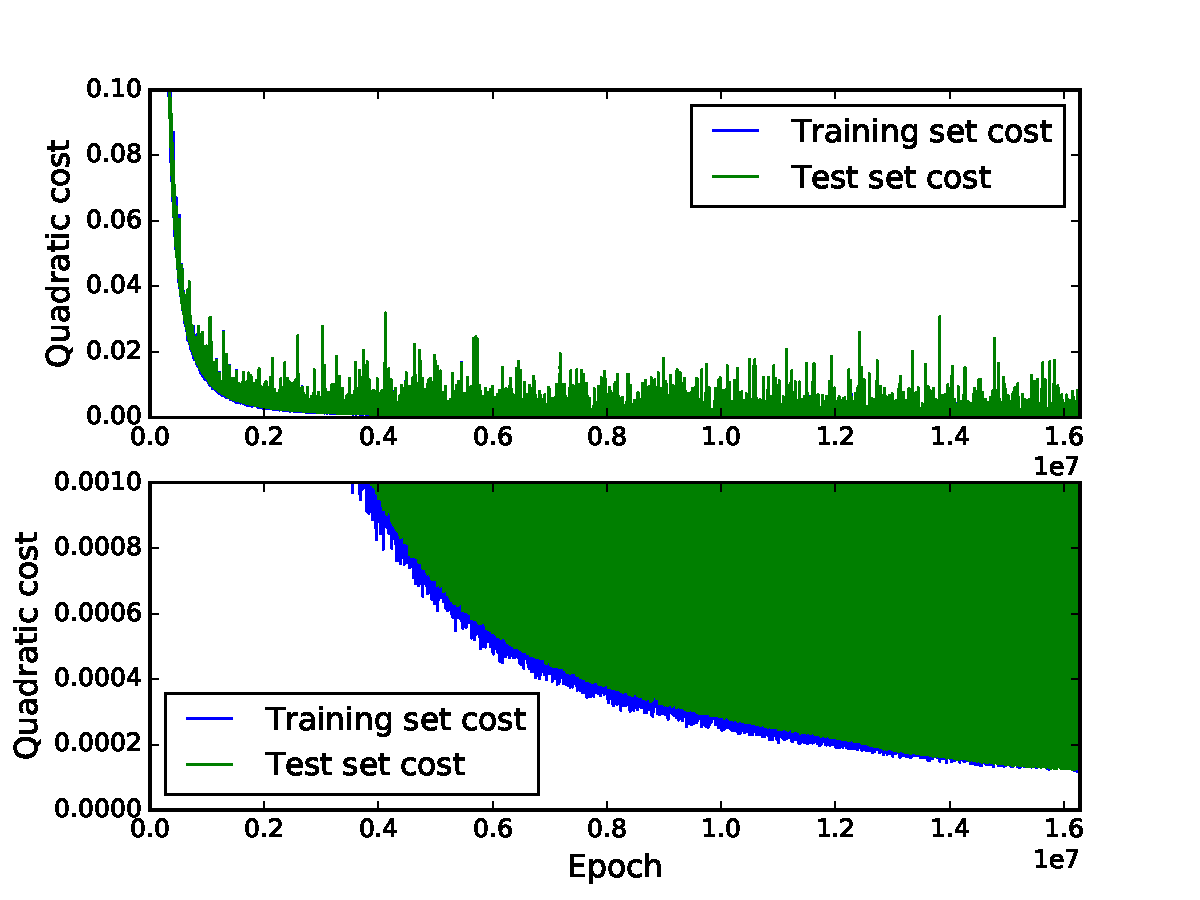
\includegraphics[width=0.8\textwidth]{Figures/Tests/trainingManyNeighbourNN2.pdf}}
\caption{Quadratic cost \eqref{quadraticCostFunction} of training set and test set for NN trained to yield
	 the sum of the shifted LJ-potential of 20 neighbouring atoms. 
	 The NN has 20 inputs, one hidden layer 
	 with 200 neurons and one output node. All nodes in the hidden layer have sigmoid activation functions 
	 \eqref{sigmoidActivationFunction}. \autoref{zoomedOut} shows the cost for the first 50 000 epochs, while
	 \autoref{zoomedIn} displays the cost for all epochs, but on a smaller scale.}	 
\label{fig:trainingManyNeighbourNN}
\end{figure}
The cost rapidly decreases during the first 10 000 epochs, then it starts to flatten out. This behaviour seems
to be general when doing regression with ANNs. 
There is no sign of overfitting: we do not observe an increase in the test cost relative to the training cost. 
This is (PROBABLY) due to the fact that our training set and test set are random numbers, i.e. there will be no 
specifics patterns or configurations present in the test set that is not covered by the training set. 
When we start doing training on data produced by MD trajectories or QM calculations, the situation will different.

The NN above outputs the total energy on an atom that is surrounded by $N$ neighbouring atoms, but it does not provide the forces. 
These must be obtained by calculating the analytical derivative of the NN with backpropagation as described above for each time step.
An alternative approach that may speed up the MD simulation is to have the NN also output the total force on the central atom. 
This can be done giving the cartesian coordinates and distance of N atoms as input to the NN so that each input
vector looks like
\begin{equation}
 (x_1, y_1, z_1, r_1, x_2, y_2, z_2, r_2, \dots, x_N, y_N, z_N, r_N)
\end{equation}
which yields an output vector
\begin{equation}
 (F_x^{TOT}, F_y^{TOT}, F_z^{TOT}, E^{TOT})
\end{equation}
We have to make sure that the input coordinates are in the range 
$x, y, z \in [-r_{cut}, r_{cut}]$ to cover the whole configuration space. The distances however, are still in the range
$r \in [a, r_{cut}]$ where $a$ is the minimum distance that two atoms can have in a given MD simulation (see function
\textit{energyAndForceCoordinates} in \textit{generateData}). As the NN now have 4 inputs per neighbour and 4 outputs, 
we need to have more nodes to get a sufficiently low error. We run a training session with 5 neighbours (20 inputs) 
(session 13.12-12.59.51). The cost has the same shape as before, but the error is much larger to begin with and also converges
slower (SKAL JEG GIDDE Å HA ENDA ET ERROR PLOT HER?).

One way to test if this works is to move only one of the input atoms while freezing the others and see if we reproduce
the LJ-potential form. We load the above training session and test with the command 
python approximateFunction2.py --load TrainingData/13.12-12.59.51/Checkpoints/ckpt-999 --test with this code: 
\begin{lstlisting}
if testFlag:
  
  # pick an input vector
  coordinates = xTrain[0]
  coordinates = coordinates.reshape([1,self.inputs])
  neighbours = self.inputs/4
  xNN = np.zeros(neighbours)
  yNN = np.zeros(neighbours)
  zNN = np.zeros(neighbours)
  rNN = np.zeros(neighbours)
  # extract coordinates and distances
  for i in range(neighbours):
      xNN[i] = coordinates[0,i*4]
      yNN[i] = coordinates[0,i*4 + 1]
      zNN[i] = coordinates[0,i*4 + 2]
      rNN[i] = coordinates[0,i*4 + 3]
		  
  # vary coordinates of only one atom and see 
  # if the resulting potential is similar to LJ
  N = 500
  r = np.linspace(0.8, 2.5, N)
  energyNN = []
  energyLJ = []
  forceNN = []
  forceLJ = []
  xyz = np.zeros(3)
  for i in range(N):
      r2 = r[i]**2
      xyz[0] = np.random.uniform(0, r2)
      xyz[1] = np.random.uniform(0, r2-xyz[0])
      xyz[2] = r2 - xyz[0] - xyz[1]
      #np.random.shuffle(xyz)
      x = np.sqrt(xyz[0])# * np.random.choice([-1,1])
      y = np.sqrt(xyz[1])# * np.random.choice([-1,1])
      z = np.sqrt(xyz[2])# * np.random.choice([-1,1])                      
      coordinates[0][0] = x; coordinates[0][1] = y; coordinates[0][2] = z
      coordinates[0][3] = r[i]
      energyAndForce = sess.run(prediction, feed_dict={self.x: coordinates})
      energyNN.append(energyAndForce[0][3]) 
      rNN[0] = r[i]
      energyLJ.append(np.sum(self.function(rNN)))
      forceNN.append(energyAndForce[0][0])
      xNN[0] = x
      forceLJ.append(np.sum(self.functionDerivative(rNN)*xNN/rNN))
  
  # convert to arrays
  energyNN = np.array(energyNN); energyLJ = np.array(energyLJ)
  forceNN = np.array(forceNN); forceLJ = np.array(forceLJ)
  
  # plot error 
  plt.plot(r, energyNN - energyLJ)
  plt.show()
  plt.plot(r, forceNN - forceLJ)
  plt.show()
  print 'Cost: ', (np.sum((energyNN - energyLJ)**2 + (forceNN - forceLJ)**2))/N
  
  # see if the energy is zero when all neighbours is at cutoff distance
  inputz = np.array([1.87, 1.32, 1.006, 2.5]*neighbours).reshape([1,self.inputs])
  r = np.array([2.5]*neighbours)
  energyLJ = sum(self.function(r))               
  ef = sess.run(prediction, feed_dict={self.x: inputz})
  
  print 'Approximate energy: ', ef[0,3]
  print 'LJ energy: ', energyLJ
  
  numberOfEpochs = 0
\end{lstlisting}
which produces the following output: 
\begin{lstlisting}
Model restored
Cost:  0.132622806039
NN energy at cutoff:  0.125104
LJ energy at cutoff:  0.0
Time elapsed: 1.2e-05
\end{lstlisting}
We see that the NN energy at cutoff is not zero, because of the cost (IS THIS CORRECT? THE COST AT CUTOFF IS PRACTICALLY ZERO).
The error of the NN energy and forces over the training data interval is shown in 
\begin{figure}[H]
\begin{minipage}[t]{0.48\linewidth}
  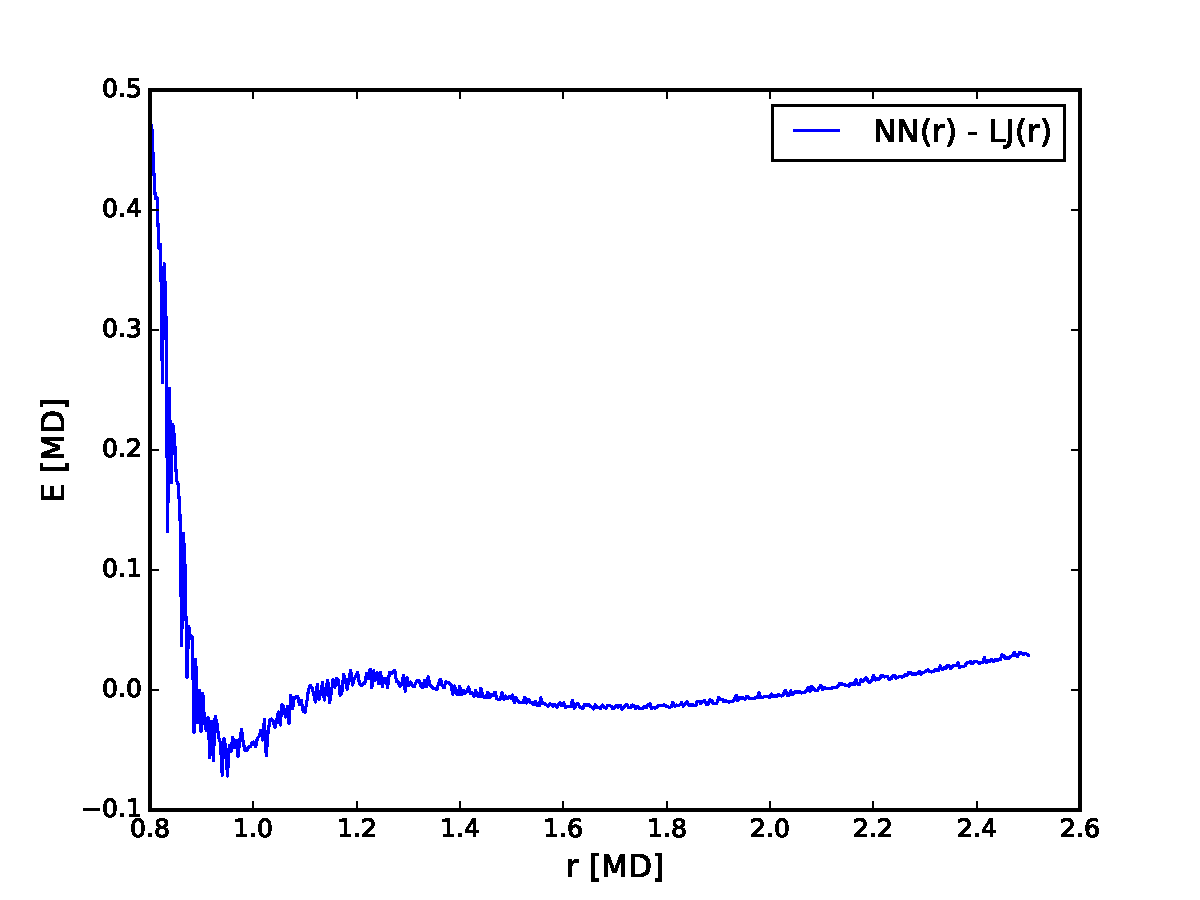
\includegraphics[width=\textwidth]{Figures/Tests/manyNeighbourEnergyError.pdf}
\end{minipage}
\quad
\begin{minipage}[t]{0.48\linewidth}
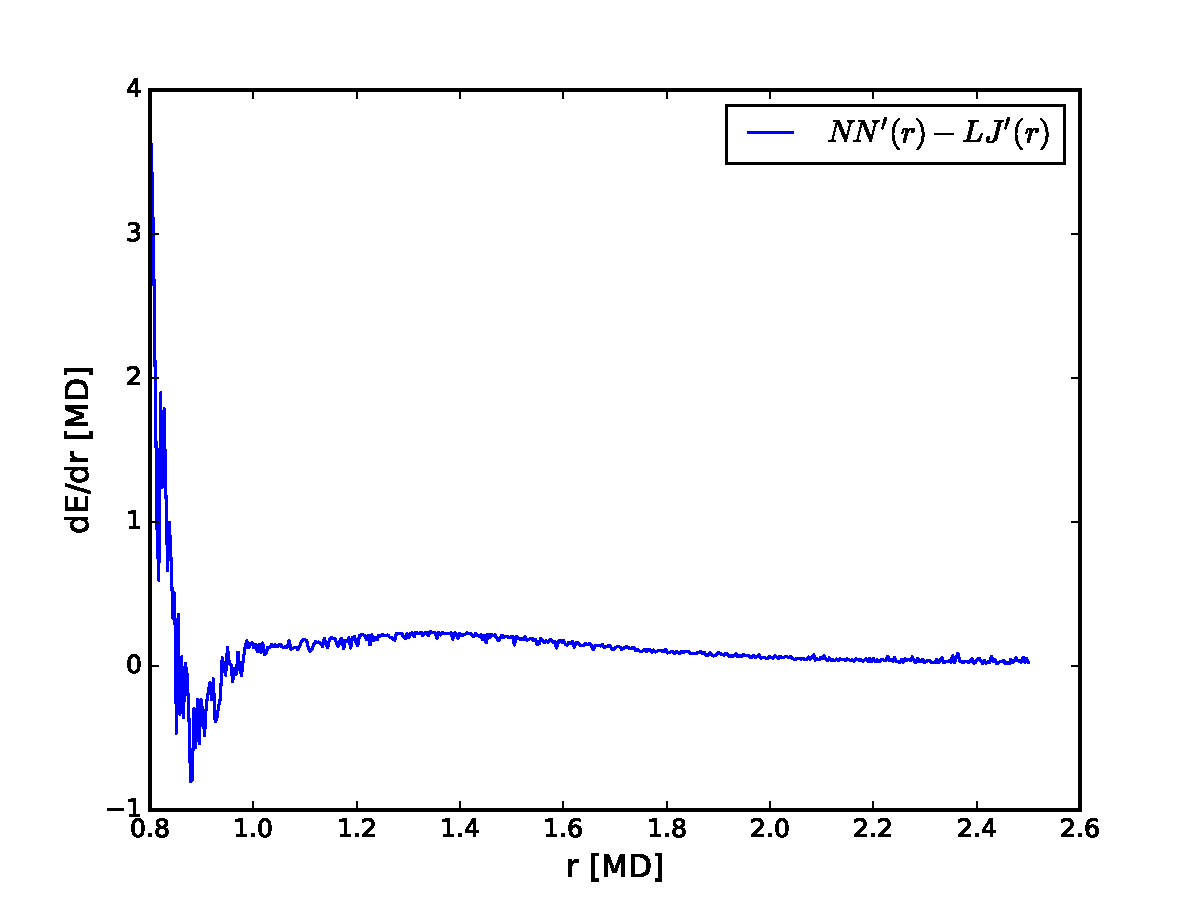
\includegraphics[width=\textwidth]{Figures/Tests/manyNeighbourForceError.pdf}
\end{minipage}
  \caption{Error of a network trained to yield the total energy and force on a central atom from 5 neighbouring atoms. 
           The energy contribution from each neighbour is a shifted LJ potential. Trained for 1e6 epochs, 100 nodes
           in 2 layers. The energy error is shown on the left, force error on the right.}
\label{fig:errorManyNeighbourNN}
\end{figure}
The error oscillates in exactly the same way as for the 1-input NN above, suggesting that the training is done correctly. 
However, it is very important that the energies and forces in an MD simulation is consistent, and this is not 
ensured here, where the two are obtained in a somewhat independent way. Any incosistency between the energies and forces
will magnify for each time step, resulting in inaccurate statistical properties like temperature and pressure. 
Therefore it is a better idea to have the NN only output the total energy, and find the forces by analytically
differentiating the NN for each time step. $\SI{4}{\angstrom}$

\part{Results and discussion}

\section{NN potential for Si}
Construct an NN potential for Si that works in a certain temperature range (only solid, or liquid too?)
Compute thermodynamic properties and things like radial distrubution function and compare both 
with experiments and with results with Stillinger-Weber. 

\section{NN potential for SiO2}
Construct an NN potential for SiO2 that works in a certain temperature range (only solid, or liquid too?). 
Can use various potentials as the black box, e.g. Vashishta or ReaxFF. 
ReaxFF would be great, because then we would maybe get a speed-up. 


\begin{appendices}

\chapter{Symmetry functions derivatives} \label{app:appendixA1}
We list here the derivatives of the symmetry functions used for training neural networks. These have to be known
to compute forces for MD simulations. In some cases we only show the deriviative with respect to 
$R = \sqrt{x^2 + y^2 + z^2}$. 
Each component $\alpha$ can be calculated by
\begin{equation}
 \frac{\partial R}{\partial \alpha} = \frac{\alpha}{R}
\end{equation}
The following notation applies in the following,
\begin{equation}
 R_{ij} = \Bigr(x_{ij}^2 + y_{ij}^2 + z_{ij}^2\Bigr)^{1/2} =
 \Bigr((x_j - x_i)^2 + (y_j - y_i)^2 + (z_j - z_i)^2\Bigr)^{1/2}
\end{equation}
Cutoff function \eqref{cutoffFunction}:
\begin{equation}
 \frac{\partial f_c(R)}{\partial R} = -\frac{1}{2}\frac{\pi}{R_c} \sin\left(\frac{\pi R}{R_c}\right) = M(R)
 \label{cutOffFunctionDerivative}
\end{equation}
This expression is valid for all combinations of indicies. The derivatives w.r.t. to individual coordinates are
\begin{equation}
 \frac{\partial f_c(R_{ij})}{\partial x_{ij}} = M(R_{ij})
 \frac{x_{ij}}{R_{ij}}
 \label{cutOffFunctionDerivative1}
\end{equation}
and 
\begin{equation}
 \frac{\partial f_c(R_{ik})}{\partial x_{ik}} = M(R_{ik})
 \frac{x_{ik}}{R_{ik}}
 \label{cutOffFunctionDerivative1}
\end{equation}
while
\begin{equation}
 \frac{\partial f_c(R_{ij})}{\partial x_{ik}} = \frac{\partial f_c(R_{ik})}{\partial x_{ij}} = 0
\end{equation}
because atom $i$ is always in origo, which means we can do the substitutions $x_{ij} \rightarrow x_{j}$ and 
$x_{ik} \rightarrow x_{k}$. SHOULD I DO THIS CONSEQUENTLY BELOW????. Also, 
\begin{equation}
 \frac{\partial f_c(R_{jk})}{\partial x_{ij}} = -M(R_{jk})
 \frac{x_{jk}}{R_{jk}}
 \label{cutOffFunctionDerivative1}
\end{equation}
and 
\begin{equation}
 \frac{\partial f_c(R_{jk})}{\partial x_{ij}} = M(R_{jk})
 \frac{x_{jk}}{R_{jk}}
 \label{cutOffFunctionDerivative1}
\end{equation}
The derivative of each term in $G_i^1$ \eqref{G1} is simply \eqref{cutOffFunctionDerivative}. \\
$G_i^2$ \eqref{G2}:
\begin{equation}
 \frac{\partial G_i^2}{R_{ij}} = 
 \exp(-\eta(R_{ij}-R_s)^2) \left[2\eta(R_s - R_{ij}) + \frac{\partial f_c}{\partial R_{ij}}\right]
\end{equation}
$G_i^3$ has not been used in this theses. \\
$G_i^4$ \eqref{G4}:
\begin{equation}
 G_i^4 = F_1(\theta)F_2(R_{ij},R_{ik},R_{jk})F_3(R_{ij},R_{ij},R_{jk})
\end{equation}
where
\begin{align}
 F_1(\theta) &= 2^{1-\zeta}(1 + \lambda \cos\theta_{ijk})^\zeta \\
 F_2(R_{ij},R_{ik},R_{jk}) &= \exp[-\eta (R_{ij}^2 + R_{ik}^2 + R_{jk}^2)] \\
 F_3(R_{ij},R_{ij},R_{jk}) &= f_c(R_{ij}) f_c(R_{ik}) f_c (R_{jk})
\end{align}
where
\begin{equation}
 \cos\theta = \frac{x_{ij}x_{ik} + y_{ij}y_{ik} + z_{ij}z_{ik}}{R_{ij}R_{ik}}
\end{equation}
Using the product rule:
\begin{align}
 \frac{\partial G_i^4}{\partial x_{ij}} = &\frac{\partial F_1}{x_{ij}} F_2 F_3 + 
 F_1 \left(\frac{\partial F_2}{\partial x_{ij}}F_3 + F_2\frac{\partial F_3}{\partial x_{ij}}\right) \\
 &\frac{\partial F_1}{x_{ij}} F_2 F_3 + 
 F_1 \frac{\partial F_2}{\partial x_{ij}}F_3 + F_1F_2\frac{\partial F_3}{\partial x_{ij}}
 \label{G4Derivative}
\end{align}
We have
\begin{equation}
 \frac{\partial F_1}{\partial x_{ij}} = \frac{\partial F_1}{\partial\cos\theta}
 \frac{\partial\cos\theta}{\partial x_{ij}}
\end{equation}
where
\begin{equation}
 \frac{\partial F_1}{\partial\cos\theta} = \lambda\zeta(1 + \cos\theta)^{\zeta-1} = K
\end{equation}
and 
\begin{equation}
 \frac{\partial\cos\theta}{\partial x_{ij}} = \frac{x_{ik}}{r_{ij}r_{ik}} - 
 \frac{x_{ij}\cos\theta}{r_{ij}^2}
\end{equation}
To get the corresponding expression for $x_{ik}$, simply substitute $x_{ij} \leftrightarrow x_{ik}$ and 
$r_{ij} \leftrightarrow r_{ik}$. Further, 
\begin{align}
 \frac{\partial F_2}{\partial x_{ij}} &= \frac{\partial F_2}{\partial r_{ij}}\frac{\partial r_{ij}}{\partial x_{ij}}  = 
 (-2\eta r_{ij}\frac{x_{ij}}{r_{ij}} - 2\eta r_{jk}\frac{x_{jk}}{r_{jk}})\exp[-\eta (R_{ij}^2 + R_{ik}^2 + R_{jk}^2)] \\
 &= -2\eta F_2 x_{ij} - 2\eta F_2 x_{jk}
\end{align}
The corresponding expression for $x_{ik}$ is
\begin{equation}
 \frac{\partial F_2}{\partial x_{ik}} = 
 -2\eta F_2 x_{ik} + 2\eta F_2 x_{jk}
\end{equation}
Lastly, 
\begin{align}
 \frac{\partial F_3}{\partial x_{ij}} &=  \frac{\partial f_c(r_{ij})}{\partial x_{ij}}
 f_c(r_{ik}) f_c(r_{jk}) + f_c(r_{ij})f_c(r_{ik})\frac{\partial f_c(r_{jk})}{\partial x_{ij}} \\
 &= f_c(r_{ik})\Biggr(M(r_{ij})\frac{x_{ij}}{r_{ij}}f_c(r_{jk}) - 
 f_c(r_{ij}) M(r_{jk})\frac{x_{jk}}{r_{jk}} \Biggr)
\end{align}
The corresponding expression for $x_{ik}$ is
\begin{align}
 \frac{\partial F_3}{\partial x_{ik}} &= f_c(r_{ij})\Biggr(\frac{\partial f_c(r_{ik})}{\partial x_{ik}}f_c(r_{jk}) + 
 f_c(r_{ik}) \frac{\partial f_c(r_{jk})}{\partial x_{ik}} \Biggr) \\
 &= f_c(r_{ij})\Biggr(M(r_{ik})\frac{x_{ik}}{r_{ik}}f_c(r_{jk}) + 
 f_c(r_{ik}) M(r_{jk})\frac{x_{jk}}{r_{jk}} \Biggr) \\
\end{align}
Then, taking \eqref{G4Derivative} into account:
\begin{align}
 \frac{\partial G_i^4}{\partial x_{ij}} = &\biggr(\frac{x_{ik}}{r_{ij}r_{ik}} - \frac{x_{ij}\cos\theta}{r_{ij}^2}
 \biggr)KF_2F_3 \, - \\ &2\eta F_1F_2F_3 x_{jk} - 2\eta F_1F_2F_3 x_{ij} \, + \\
 &F_1F_2 f_c(r_{ik})\Biggr(M(r_{ij})\frac{x_{ij}}{r_{ij}}f_c(r_{jk}) +
 f_c(r_{ij}) M(r_{jk})\frac{x_{jk}}{r_{jk}} \Biggr)
\end{align}
and for $x_{ik}$:
\begin{align}
 \frac{\partial G_i^4}{\partial x_{ik}} = &\biggr(\frac{x_{ij}}{r_{ij}r_{ik}} - \frac{x_{ik}\cos\theta}{r_{ik}^2}
 \biggr)KF_2F_3 \, + \\ &2\eta F_1F_2F_3 x_{jk} - 2\eta F_1F_2F_3 x_{ik} \, + \\
 &F_1F_2 f_c(r_{ij})\Biggr(M(r_{ik})\frac{x_{ik}}{r_{ik}}f_c(r_{jk}) - 
 f_c(r_{ik}) M(r_{jk})\frac{x_{jk}}{r_{jk}} \Biggr)
\end{align}
or in terms of $x_{ij}$ and $x_{ik}$ and $x_{jk}$:
\begin{align}
 \frac{\partial G_i^4}{\partial x_{ij}} = &x_{ij} \biggr(-\frac{\cos\theta}{r_{ij}^2}K
 F_2F_3 - 2\eta F_1F_2F_3 \, + \\ 
 &F_1F_2M(r_{ij})f_c(r_{ik})f_c(r_{jk})\frac{1}{r_{ij}}\biggr) \, + \\
 &x_{ik}\frac{KF_2F_3}{r_{ij}r_{ik}} - x_{jk}\Bigr(F_1F_2M(r_{jk})f_c(r_{ik})f_c(r_{ij}) + 2\eta F_1F_2F_3\Bigr)\frac{1}{r_{jk}}
\end{align}
and 
\begin{align}
 \frac{\partial G_i^4}{\partial x_{ik}} = &\frac{x_{ik}}{r_{ik}} \biggr(-\frac{\cos\theta}{r_{ik}^2}K
 F_2F_3 - 2\eta F_1F_2F_3 \, + \, \\
 &F_1F_2M(r_{ik})f_c(r_{ij})f_c(r_{jk})\frac{1}{r_{ik}}\biggr) + \, \\
 &x_{ij}\frac{KF_2F_3}{r_{ij}r_{ik}} + x_{jk}\Bigr(F_1F_2M(r_{jk})f_c(r_{ij})f_c(r_{ik}) - 2\eta F_1F_2F_3\Bigr)\frac{1}{r_{jk}}
\end{align}
The derivative of $G_i^5$ \eqref{G5} is found in a similar way,
\begin{equation}
 G_i^5 = F_1(\theta)F_2(R_{ij},R_{ik})F_3(R_{ij},R_{ij})
\end{equation}
where 
\begin{align}
 F_1(\theta) &= 2^{1-\zeta}(1 + \lambda \cos\theta_{ijk})^\zeta \\
 F_2(R_{ij},R_{ik}) &= \exp[-\eta (R_{ij}^2 + R_{ik}^2)] \\
 F_3(R_{ij},R_{ij}) &= f_c(R_{ij}) f_c(R_{ik})
\end{align}
The derivative of $F_1$ is the same, while for $F_2$ we obtain
\begin{equation}
 \frac{\partial F_2}{\partial x_{ij}} = -2\eta F_2 x_{ij}
\end{equation}
and
\begin{equation}
 \frac{\partial F_2}{\partial x_{ik}} = -2\eta F_2 x_{ik}
\end{equation}
For $F_3$, 
\begin{equation}
 \frac{\partial F_3}{\partial x_{ij}} = \frac{\partial f_c(r_{ij})}{\partial x_{ij}}\frac{x_{ij}}{r_{ij}}
 f_c(r_{ik}) = M(r_{ij})f_c(r_{ik})\frac{x_{ij}}{r_{ij}}
\end{equation}
and
\begin{equation}
  \frac{\partial F_3}{\partial x_{ik}} = f_c(r_{ij})
 \frac{\partial f_c(r_{ik})}{\partial x_{ij}}\frac{x_{ik}}{r_{ik}} = 
 f_c(r_{ij})M(r_{ik})\frac{x_{ik}}{r_{ik}}
\end{equation}
so that
\begin{align}
 \frac{\partial G_i^5}{\partial x_{ij}} = &\biggr(\frac{x_{ik}}{r_{ij}r_{ik}} - \frac{x_{ij}\cos\theta}{r_{ij}^2}
 \biggr)KF_2F_3 -
 2\eta F_1 F_2F_3 x_{ij} \, + \\
 &F_1F_2 M(r_{ij})f_c(r_{ik})\frac{x_{ij}}{r_{ij}}
\end{align}
and 
\begin{align}
 \frac{\partial G_i^5}{\partial x_{ik}} = &\biggr(\frac{x_{ij}}{r_{ij}r_{ik}} - \frac{x_{ij}\cos\theta}{r_{ik}^2}
 \biggr)KF_2F_3 -
 2\eta F_1 F_2F_3 x_{ik} \, + \\
 &F_1F_2 M(r_{ik})f_c(r_{ij})\frac{x_{ik}}{r_{ik}}
\end{align}
In terms of $x_{ij}$ and $x_{ik}$:
\begin{align}
 \frac{\partial G_i^5}{\partial x_{ij}} = \, &x_{ij} \biggr(-\frac{\cos\theta}{r_{ij}^2}K
 F_2F_3 - 2\eta F_1F_2F_3 + F_1F_2M(r_{ij})f_c(r_{ik})\frac{1}{r_{ij}} \biggr) \, + \\
 &x_{ik}\frac{KF_2F_3}{r_{ij}r_{ik}}
\end{align}
and 
\begin{align}
 \frac{\partial G_i^5}{\partial x_{ik}} = \, &x_{ik} \biggr(-\frac{\cos\theta}{r_{ik}^2}K
 F_2F_3 - 2\eta F_1F_2F_3 + F_1F_2M(r_{ik})f_c(r_{ij})\frac{1}{r_{ik}} \biggr) \, + \\
 &x_{ij}\frac{KF_2F_3}{r_{ij}r_{ik}}
\end{align}


\end{appendices}





\newpage

\begin{thebibliography}{56}

\bibitem{Behler11general}
 J. Behler.
 ''Neural network potential-energy surfaces in chemistry: a tool for large-scale simulations''.
 In: \textit{Phys. Chem. Chem. Phys.} 13. (2011), 17930-17955. 
 DOI: \href{http://dx.doi.org/10.1039/c1cp21668f}{10.1039/c1cp21668f}. 
 
\bibitem{Behler11symmetry}
 J. Behler.
 ''Atom-centered symmetry functions for constructing high-dimensional neural network potentials''.
 In: \textit{The Journal of Chemical Physics} 134. (2011), 074106. 
 DOI: \href{http://dx.doi.org/10.1063/1.3553717}{10.1063/1.3553717}.
 
\bibitem{Dragly14}
 S. A. Dragly.
 ''Bridging quantum mechanics and molecular dynamics with artificial neural networks''.
 MA thesis. University of Oslo (2014). \\
 URL: \href{https://www.duo.uio.no/handle/10852/41843}{https://www.duo.uio.no/handle/10852/41843}.

\bibitem{Hornik89}
 K. Hornik, M. Stinchcombe and H. White.
 ''Multilayer Feedforward Networks are Universal Approximators''.
 In: \textit{Neural Networks} 2. (1989), 359. 
 DOI: \href{https://doi.org/10.1016/0893-6080(89)90020-8}{10.1016/0893-6080(89)90020-8}
 
\bibitem{Rojas96}
 R. Rojas. 
 \textit{Neural Networks: A Systematic Introduction}.
 Springer, 1996.
 
\bibitem{Karlik11}
 B. Karlik and A. V. Olgac.
 ''Performance Analysis of Various Activation Functions in Generalized MLP Architectures of Neural Networks''.
 In: \textit{IJAE} 1. (2011), 111-122.
 
\bibitem{LeCun15}
 Y. LeCun, Y. Bengio and G. Hinton.
 ''Deep learning''.
 In: \textit{Nature} 521. (2015), 436-444. 
 DOI: \href{http://dx.doi.org/10.1038/nature14539}{10.1038/nature14539}
 
\bibitem{Glorot11}
 X. Glorot, A. Bordes, Y. Bengio.
 ''Deep Sparse Rectifier Neural Networks''.
 In: \textit{JMLR} 15. (2011), 315-323.
 
\bibitem{Rumelhart86}
 D. E. Rumelhart, G. E. Hinton and R. J. Williams.
 ''Learning representations by back-propagating errors''.
 In: \textit{Nature} 323. (1986), 533-536.
 DOI: \href{http://dx.doi.org/10.1038/323533a0}{10.1038/323533a0}
 
\bibitem{Behler15}
 J. Behler.
 ''Constructing High-Dimensional Neural Network Potentials: A Tutorial Review''.
 In: \textit{International Journal of Quantum Chemistry} 115. (2015), 1032-1050.
 DOI: \href{http://dx.doi.org/10.1002/qua.24890}{10.1002/qua.24890}
 
\bibitem{Tuckerman92}
 Tuckerman, Berne and Martyna .
 ''Reversible multiscale molecular dynamics''.
 In: \textit{J. Chem. Phys.} 97. (1992), 1990.
 
\bibitem{Plimpton95}
 S. Plimpton. 
 ''Fast Parallel Algorithms for Short-Range Molecular Dynamics''.
 In: \textit{Journal of Computational Physics} 117. (1995) 1-19. 
 DOI: \href{https://doi.org/10.1006/jcph.1995.1039}{10.1006/jcph.1995.1039}. 
 
\bibitem{Abadi15}
 M. Abadi, A. Agarwal, P. Barham, E. Brevdo,
 Z. Chen, C. Citro, G. S. Corrado, A. Davis,
 J. Dean, M. Devin, S. Ghemawat, I. Goodfellow,
 A. Harp, G. Irving, M. Isard, R. Jozefowicz, Y. Jia,
 L. Kaiser, M. Kudlur, J. Levenberg, D. Mané, M. Schuster,
 R. Monga, S. Moore, D. Murray, C. Olah, J. Shlens,
 B. Steiner, I. Sutskever, K. Talwar, P. Tucker,
 V. Vanhoucke, V. Vasudevan, F. Viégas,
 O. Vinyals, P. Warden, M. Wattenberg, M. Wicke,
 Y. Yu and X. Zheng.
 ''TensorFlow: Large-scale machine learning on heterogeneous systems''.
 \textit{Google Research} (2015). 
 arXiv: \href{https://arxiv.org/abs/1603.04467}{1603.04467}
 
\bibitem{Abadi16}
 M. Abadi, P. Barham, J. Chen, Z. Chen, A. Davis, J. Dean,
 M. Devin, S. Ghemawat, G. Irving, M. Isard, M. Kudlur,
 J. Levenberg, R. Monga, S. Moore, D. G. Murray, B. Steiner, P. Tucker,
 V. Vasudevan, P. Warden, M. Wicke, Y. Yu, and X. Zheng.
 ''TensorFlow: A System for Large-Scale Machine Learning''.
 \textit{Google Brain} (2016).
 arXiv: \href{https://arxiv.org/abs/1605.08695}{1605.08695}
 
\bibitem{Qian99}
 N. Qian.
 ''On the momentum term in gradient descent learning algorithms''
 In: \textit{Neural Networks} 12(1). (1999) 145-151. 
 DOI: \href{https://doi.org/10.1016/S0893-6080(98)00116-6}{10.1016/S0893-6080(98)00116-6}
 
\bibitem{Duchi11}
 J. Duchi, E. Hazan, Y. Singer.
 ''Adaptive Subgradient Methods for Online Learning and Stochastic Optimization''.
 In \textit{The Journal of Machine Learning Research} 12. (2011) 2121-2159. 
 URL: \href{http://jmlr.org/papers/v12/duchi11a.html}{http://jmlr.org/papers/v12/duchi11a.html}
 
\bibitem{Zeiler12}
 M. D. Zeiler. 
 ''Adadelta: an adaptive learning rate method''. (2012).
 arXiv: \href{https://arxiv.org/abs/1212.5701}{1212.5701}
 
\bibitem{Kingma14}
 D. P. Kingma and J. Ba.
 ''Adam: A Method for Stochastic Optimization''. (2014).
 arXiv: \href{https://arxiv.org/abs/1412.6980}{1412.6980}
 
\bibitem{Ischtwan94}
 J. Ischtwan and M. A. Collins.
 ''Molecular potential energy surfaces by interpolation''.
 In: \textit{The Journal of Chemical Physics} 100. (1994), 8080.
 DOI: \href{http://dx.doi.org/10.1063/1.466801}{10.1063/1.466801}
 
\bibitem{Raff05}
 L. M. Raff, M. Malshe, M. Hagan, D. I. Doughan, M. G. Rockley and R. Komanduri.
 ''Ab inito potential-energy surfaces for complex, multichannel systems using modified
 novelty sampling and feedforward neural networks''. 
 In: \textit{The Journal of Chemical Physics} 122. (2005), 084104. 
 DOI: \href{http://dx.doi.org/10.1063/1.1850458}{10.1063/1.1850458}
 
\bibitem{Raff12}
 L. M. Raff, R. Komanduri, M. Hagan and S. T. S. Bukkapatnam 
 \textit{Neural networks in chemical reaction dynamics}.
 Oxford University Press, 2012.
 
\bibitem{Pukrittayakamee09}
 A. Pukrittayakamee, M. Malshe, M. Hagan, L. M. Raff, R. Narulkar, 
 S. Bukkapatnum and R. Komanduri. 
 ''Simultaneous fitting of a potential-energy surface and its corresponding force fields
 using feedforward neural networks''. 
 In: \textit{The Journal of Chemical Physics}
 DOI: \href{http://dx.doi.org/10.1063/1.3095491}{10.1063/1.3095491}
 

 
 
\end{thebibliography}

\end{document}